%\documentclass[handout]{beamer}
\documentclass{beamer}

\usepackage{color}
\usepackage{beamerthemesplit}
\usepackage[utf8]{inputenc}
\usepackage{graphicx}
%\usetheme{Malmoe}
%\usetheme{CambridgeUS}
%\usetheme{Hannover}
\usepackage{watermark}
\usepackage{eso-pic}
\usepackage{comment}
% Tema Simple
\usetheme[height=0.35cm]{Madrid}

% El que uso habitualmente:
%\usetheme[height=0.7cm]{Rochester}

% A dark look
%\usecolortheme{beetle}
\usecolortheme{dolphin}

\setbeamertemplate{navigation symbols}{} 

%\usepackage{wrapfig}
\setbeamercovered{transparent}

\usepackage{geometry}
%\geometry{landscape}
\usepackage{multimedia}
\usepackage{verbatim}
\usepackage{bm}%bold matH

%\usepackage{shade}
\usepackage{fancybox}
\usepackage{amssymb}
%------------ VIDEO---------------
\usepackage{hyperref}
\usepackage{media9}%
\usepackage{multimedia}

%\input{embed_video}

%\newcommand{\includemovie}[3]{%
%\includemedia[%
%width=#1,height=#2,%
%activate=pagevisible,%
%deactivate=pageclose,%
%addresource=#3,%
%flashvars={%
%src=#3 % same path as in addresource!
%&autoPlay=true % default: false; if =true, automatically starts playback after activation (see option ‘activation)’
%&loop=true % if loop=true, media is played in a loop
%&controlBarAutoHideTimeout=0 %  time span before auto-hide
%}%
%]{}{StrobeMediaPlayback.swf}%
%--------------------------------

% Defino clases de secciones en ESPAÑOL
\def\chaptername{Cap\'\i tulo}
\def\abstractname{Resumen}
\def\contentsname{Contenidos}
\def\bibname{Bibliograf\'\i a}
\def\appendixname{Ap\'endice}
\def\tablename{\textbf{Tabla}}
\def\figurename{\textbf{Figura}}
%\usepackage[dvips]{graphics,color,epsfig}
%\usepackage{pst-all}
%\usepackage{pstricks}
%\topmargin=-2cm  

% Defino formatos
\def\titulo#1{\frametitle{{\ \hfill {\bf #1}}}}
\def\figu#1{\shadowbox{#1}}

\def\Eeuv{E_{\rm{EUV}}}
\def\Ewl{E_{\rm{WL}}}
\def\AvgNE2{\left<N_e^2\right>}
\def\AvgNe{\left<N_e\right>}
\def\SigmaNe{\sigma_{Ne}}
\def\VarNe{\rm{Var}N_e}
\def\AvgTe{\left<T_e\right>}
\def\SigmaTe{\sigma_{Te}}


%EStilo
%\input{epsf.sty}

%Paquetes a utilizar

%\usepackage{amssymb} % Math
%\usepackage{graphicx}
%\usepackage{float}
%%\usepackage{wrapfig}
%%\usepackage{deluxetable}

\pagenumbering{arabic}
%\usepackage[dvips]{graphics,color}
%\usepackage{natbib}
%\usepackage{amssymb} % Math
%\usepackage{amsmath} % Math
%%\usepackage{dsfont} % Math
%\usepackage{float}
%\usepackage{graphicx}
%%\usepackage{wrapfig}
%\usepackage{pst-all}
%%\usepackage{multirow} % Multi filas

%Separacion silabica:
%%\usepackage[T1]{babel} % silabas y hyphenation
%\hyphenation{e-vi-den-cia}
%\hyphenation{an-te-rio-res}

% Control de Márgenes

%-------------------- Comandos de los autores ----------------------------

% Nombres de Journals
\newcommand{\araa}{Annu. Rev. Astron. Astrophys.}
\newcommand{\solphys}{Solar Phys.}
\newcommand{\aapr}{Astron. Astrophys. Rev.}
\newcommand{\aaps}{Astron. Astrophys. Sup. Ser.}
\newcommand{\jastp}{Jour. Atmos. Solar-Terrestrial Phys.}
\newcommand{\pasj}{Pub. Astron. Soc. Japan}
\newcommand{\etal}{et al.\ }
\newcommand{\ha}{H$\alpha$ }
\newcommand{\aap}{Astron. \& Astrophys.}
\newcommand{\apjs}{Astrophys J. Sup.}
\newcommand{\jgr}{Journal of Geophys. Res.}
\newcommand{\grl}{Geophys. Res. Let.}
\newcommand{\pre}{Physical Rev. E}
\newcommand{\adv}{Adv. in Space Res.}
\newcommand{\SpaceS}{Space Science Reviews}
\newcommand{\planss}{Planet. Space Sci.}
\newcommand{\nat}{Nature}
\newcommand{\apj}{The Astrophysical Journal}
\newcommand{\apjS}{The Astrophysical Journal Supplement}
\newcommand{\apjl}{The Astrophysical Journal Letters}
\newcommand{\mnras}{MNRAS}
\newcommand{\pasp}{Publications of the Astronomical Society of the Pacific}
\newcommand{\apss}{Astrophys. Space Sci.}

% Formato
\def\salto{\vskip 0.3cm}
\def\mediosalto{\vskip 0.15cm}

% Math:
\def\deg{$^\circ$}
\def\Rs{{R}_\odot}
\def\rsun{R$_{\odot}$}
\def\bB{\mathbf{B}}
\def\bE{\mathbf{E}}
\def\dpar#1#2{\frac{\partial#1}{\partial#2}}
%color:
\def\red#1{{\textcolor{red}{#1}}}
\def\azul#1{{\textcolor{blue}{#1}}}

\def\Figura#1{Figura \ref{#1}}
\def\Figuras#1#2{Figuras \ref{#1} a \ref{#2}}
\def\Figurasy#1#2{Figuras \ref{#1} y \ref{#2}}
\def\Tabla#1{Tabla \ref{#1}}
\def\Eq#1{Ecuaci\'on (\ref{#1})}
\def\Eqs#1#2{Ecuaciones (\ref{#1})-(\ref{#2})}
\def\Eqn#1{Ecuaci\'on (\ref{#1})}
\def\eqsy#1#2{Ecuaciones (\ref{#1}) y (\ref{#2})}

\def\exp{{\rm exp}}
\def\ln{{\rm ln}}
\def\sin#1{{\rm sen}(#1)}
\def\cos#1{{\rm cos}(#1)}
\def\sec{{\rm sec}}
\def\erg{{\rm erg}}
\def\cm{{\rm cm}}
\def\km{{\rm km}}
\def\sr{{\rm sr}}
\def\Hz{{\rm Hz}}
\def\GHz{{\rm GHz}}
\def\kev{{\rm kev}}
\def\sfu{{\rm SFU}}
\def\K{{\rm K}}
\def\MK{{\rm MK}}
\def\AU{{\rm UA}}
\def\UA{{\rm UA}}
\def\Log10{{\rm log_{10}}}
\def\G{{\rm G}}
\def\gsun{g_{\odot}}
\def\Rsun{R_{\odot}}
\def\Msun{ M_{\odot}}
\def\Ne{N_\mathrm{e}}
\def\NH{N_\mathrm{H}}
\def\NHe{N_\mathrm{He}}
\def\me{m_\mathrm{e}}
\def\mH{m_\mathrm{H}}
\def\mHe{m_\mathrm{He}}
\def\Tm{T_m}
\def\Tfit{T_{\rm fit}}
\def\Tefit{T_{e,{\rm fit}}}
\def\Te{T_{\rm e}}
\def\TH{T_{\rm H}}
\def\THe{T_{\rm He}}
\def\l{\lambda_{{\rm N}}}
\def\WT{W_{T}}
\def\aTm{\left<\Tm\right>}
\def\dT{\Delta T}
\def\emisin{\zeta_k^{\rm (syn)}}
\def\emitom{\zeta_k^{\rm(tom)}}

\def\fa{f_{\alpha} ({\bf x},{\bf w},t)}
\def\ffa{f_\alpha}
\def\xt{({\bf x},t)}
\def\vt{({\bf v},t)}
\def\xw{({\bf x},{\bf w})}
\def\xwt{({\bf x},{\bf w},t)}
\def\fa{f_\alpha}
\def\ww{{\bf w}}
\def\xx{{\bf x}}
\def\uu{{\bf u}}
\def\kk{{\bf k}}
\def\V{{\bf V}}
\def\ga{{\bf \Gamma}}

\def\lD{\lambda_D}
\def\ve{v_{Te}}
\def\we{\omega_e}
%\def\me{m_e}

\def\dgdv{ \frac{\partial g}{\partial v} }

\def\dndt{ \frac{\partial n}{\partial t} }
\def\drhodt{ \frac{\partial \rho}{\partial t} }

\def\dfdt{ {{\partial f} \over {\partial t}} }
\def\dfdx{ {{\partial f} \over {\partial \xx}} }
\def\dfdw{ {{\partial f} \over {\partial \ww}} }

\def\ddv{ {{\partial} \over {\partial v}} }
\def\ddt{ {{\partial} \over {\partial t}} }
\def\ddx{ {{\partial} \over {\partial \xx}} }
\def\ddw{ {{\partial} \over {\partial \ww}} }

\def\ep{\epsilon}
\def\al{\alpha}
\def\om{\omega}
\def\EF{{\bf E}}
\def\BF{{\bf B}}
\def\dl{\lambda_D}

\def\wp{\om_{pe}}
\def\P{\buildrel =\over P}

\def\intindef{\int_{0}^{\infty}}
%-----------Albert's-----------------
\def\rmax{$R_{\rm max}$}
\def\Nrad{N_r}
\def\Nlat{N_\theta}
\def\Nlon{N_\phi}
\def\bzeta{\boldsymbol{\zeta}}
\def\bI{{\boldsymbol{I}}}
\def\bW{{\bf W}}
\def\bp{{\boldsymbol{p}}}
\def\bR{{\bf R}}
\def\AFe{A_{\rm Fe}}
\def\br{{\bf r}}
\def\bl{{\boldsymbol{\lambda}}}
\def\Tab#1{Tabla \ref{#1}}
\def\Tmin{T_{\rm min}}
\def\Tmax{T_{\rm max}}
\def\intmm{\int_{\Tmin}^{\Tmax}}

%------------------------de albert

%---------- Author's commands---------------------------------

\def\bu{\textcolor{red}{\textbullet~}}
\def\tr{\bu}
\def\bbu{\textbullet~}
\def\btr{\textcolor{blue}{$\triangleright$~}}
\def\cmsq{cm$^2$}
\def\cmcu{cm$^3$}
\def\azul#1{\textcolor{blue}{#1}}
\def\rojo#1{\textcolor{red}{#1}}
\def\verde#1{\textcolor{green}{#1}}
\def\orange#1{\textcolor{orange}{#1}}
\colorlet{green}{green!60!gray}




%\def\rsun{R$_{\rm SUN}$}
\def\bA{{\bf A}}
\def\ba{{\boldsymbol{a}}}
\def\bB{{\bf B}}
\def\bb{{\bf b}}
\def\bC{{\bf C}}
\newcommand{\dd}{\mathrm{d}}
\def\bD{{\bf D}}
\def\bd{{\bf d}}
\def\be{{\boldsymbol{e}}}
\def\bF{{\bf F}}
\def\bff{{\bf f}}
\def\bg{{\bf g}}
\def\bG{{\bf G}}
\def\bh{{\bf h}}
\def\bH{{\bf H}}
\def\bi{{\bf i}}
\def\bI{{\boldsymbol{I}}}
\def\bk{{\bf k}}
\def\bK{{\bf K}}
\def\bM{{\bf M}}
\def\bn{{\boldsymbol{n}}}
\def\bv{{\boldsymbol{v}}}
\def\boo{{\boldsymbol{o}}}
\def\bp{{\boldsymbol{p}}}
\def\bP{{\bf $P$}}
\def\bq{{\boldsymbol{q}}}
\def\bQ{{\bf Q}}
\def\br{{\boldsymbol{r}}}
\def\bR{{\bf R}}
\def\bs{{\bf s}}
\def\bS{{\bf S}}
\def\bn{{\bf n}}
\def\bt{{\bf t}}
\def\bT{{\bf T}}
\def\bU{{\bf U}}
\def\bW{{\bf W}}
\def\bx{{\bf x}}
\def\by{{\bf y}}
\def\bSigma{{\bf \Sigma}}
\def\bLambda{{\bf \Lambda}}
\def\blambda{{\bf \lambda}}
\def\bN{{\bf \mathcal{N}}}
\def\bchi{\boldsymbol{\chi}}
\def\bxi{\boldsymbol{\xi}}
\def\bzeta{\boldsymbol{ \zeta}}
\newcommand{\lbl}{\mbox{\boldmath $\hat{l}$}}
\newcommand{\lpl}{\mbox{\boldmath $\hat{p}$}}
\def\deg{$^\circ$}
\def\mdeg{^\circ}
\def\bbp{{\bf p}}

%\def\tr{\textcolor{blue}{$\blacktriangleright$~}}
\def\bu{\textcolor{blue}{\textbullet~}}
\def\tr{\bu}
\def\bbu{\textbullet~}

\def\cmsq{cm$^2$}
\def\cmcu{cm$^3$}

\def\azul#1{\textcolor{blue}{#1}}
\def\rojo#1{\textcolor{red}{#1}}
\def\verde#1{\textcolor{green}{#1}}
\def\orange#1{\textcolor{orange}{#1}}
\def\cian#1{\textcolor{cyan}{#1}}

\def\bL{{\bf L}}
\def\bE{{\bf E}}
\def\bW{{\bf W}}

% Author's commands:
\newcommand{\DT}{\Delta T}
\newcommand{\Tsyn}{T_{\rm Syn}}
\newcommand{\Texp}{T_{\rm exp}}
\newcommand{\seg}{{\rm seg}}


%Simbolos
\def\izquierda{\azul{$\bf\leftarrowtail$}}
\def\derecha{\azul{$\bf\rightarrowtail$}}

%Diego:
\def\mrsun{{\rm R_\odot}}
\def\avgTe{\left<T_e\right>}
\def\bfa#1{\textcolor{blue}{\bf\tt #1}}
\def\bfr#1{\textcolor{red}{\bf\tt #1}}
\def\bfg#1{\textcolor{green}{\bf\tt #1}}
\def\med{{\rm Med}}
\def\mean{{\rm Mean}}

\def\Pl{\texttt{+}}
\def\Mi{\texttt{-}}

%Fede:
\def\azul#1{\textcolor{blue}{#1}}
\def\rojo#1{\textcolor{red}{#1}}
\def\verde#1{\textcolor{green}{#1}}
\def\orange#1{\textcolor{orange}{#1}}
\def\azul#1{\textcolor{blue}{#1}}
\def\lazul#1{\textcolor{blue}{#1}}
\def\eazul#1{\textcolor{blue}{\emph{#1}}}
\def\rrojo2#1{\textcolor{red}{\bf #1}}
\def\verde#1{\textcolor{green}{\bf #1}}
\def\rosa#1{\textcolor{pink}{\bf #1}}
\def\orange#1{\textcolor{orange}{#1}}


\newcommand{\rhoTr}{\rho(T,r)}
\def\dTm_dr{{{\rm d}T_e/{\rm d}r}}













%
% Defino clases de secciones en ESPAÑOL
\def\chaptername{Cap\'\i tulo}
\def\abstractname{Resumen}
\def\contentsname{Contenidos}
\def\bibname{Bibliograf\'\i a}
\def\appendixname{Ap\'endice}
\def\tablename{\textbf{Tabla}}
\def\figurename{\textbf{Figura}}
%\usepackage[dvips]{graphics,color,epsfig}
%\usepackage{pst-all}
%\usepackage{pstricks}
%\topmargin=-2cm  

% Defino formatos
\def\titulo#1{\frametitle{{\ \hfill {\bf #1}}}}
\def\figu#1{\shadowbox{#1}}

%EStilo
%\input{epsf.sty}

%Paquetes a utilizar

\usepackage{amssymb} % Math
\usepackage{graphicx}
%\usepackage{float}
%%\usepackage{wrapfig}
%%\usepackage{deluxetable}


\pagenumbering{arabic}
%\usepackage[dvips]{graphics,color}
%\usepackage{natbib}
%\usepackage{amssymb} % Math
%\usepackage{amsmath} % Math
%%\usepackage{dsfont} % Math
%\usepackage{float}
%\usepackage{graphicx}
%%\usepackage{wrapfig}
%\usepackage{pst-all}
%%\usepackage{multirow} % Multi filas

%Separacion silabica:
%%\usepackage[T1]{babel} % silabas y hyphenation


% Control de Márgenes

%-------------------- Comandos de los autores ----------------------------

% Nombres de Journals
\newcommand{\araa}{Annu. Rev. Astron. Astrophys.}
\newcommand{\solphys}{Solar Phys.}
\newcommand{\aapr}{Astron. Astrophys. Rev.}
\newcommand{\aaps}{Astron. Astrophys. Sup. Ser.}
\newcommand{\jastp}{Jour. Atmos. Solar-Terrestrial Phys.}
\newcommand{\pasj}{Pub. Astron. Soc. Japan}
\newcommand{\etal}{et al.\ }
\newcommand{\ha}{H$\alpha$ }
\newcommand{\aap}{Astron. \& Astrophys.}
\newcommand{\apjs}{Astrophys J. Sup.}
\newcommand{\jgr}{Journal of Geophys. Res.}
\newcommand{\grl}{Geophys. Res. Let.}
\newcommand{\pre}{Physical Rev. E}
\newcommand{\adv}{Adv. in Space Res.}
\newcommand{\SpaceS}{Space Science Reviews}
\newcommand{\planss}{Planet. Space Sci.}
\newcommand{\nat}{Nature}
\newcommand{\apj}{The Astrophysical Journal}
\newcommand{\apjS}{The Astrophysical Journal Supplement}
\newcommand{\apjl}{The Astrophysical Journal Letters}
\newcommand{\mnras}{MNRAS}
\newcommand{\pasp}{Publications of the Astronomical Society of the Pacific}
\newcommand{\apss}{Astrophys. Space Sci.}

% Formato
\def\salto{\vskip 0.3cm}
\def\mediosalto{\vskip 0.15cm}

% Math:
\def\deg{$^\circ$}
\def\rsun{R$_{\odot}$}
\def\bB{\mathbf{B}}
\def\bE{\mathbf{E}}
\def\dpar#1#2{\frac{\partial#1}{\partial#2}}
%color:
\def\red#1{{\textcolor{red}{#1}}}
\def\azul#1{{\textcolor{blue}{#1}}}

\def\Figura#1{Figura \ref{#1}}
\def\Figuras#1#2{Figuras \ref{#1} a \ref{#2}}
\def\Figurasy#1#2{Figuras \ref{#1} y \ref{#2}}
\def\Tabla#1{Tabla \ref{#1}}
\def\Eq#1{Ecuaci\'on (\ref{#1})}
\def\Eqs#1#2{Ecuaciones (\ref{#1})-(\ref{#2})}
\def\Eqn#1{Ecuaci\'on (\ref{#1})}
\def\eqsy#1#2{Ecuaciones (\ref{#1}) y (\ref{#2})}

\def\exp{{\rm exp}}
\def\ln{{\rm ln}}
\def\sin#1{{\rm sen}(#1)}
\def\cos#1{{\rm cos}(#1)}
\def\sec{{\rm sec}}
\def\erg{{\rm erg}}
\def\cm{{\rm cm}}
\def\km{{\rm km}}
\def\sr{{\rm sr}}
\def\Hz{{\rm Hz}}
\def\GHz{{\rm GHz}}
\def\kev{{\rm kev}}
\def\sfu{{\rm SFU}}
\def\K{{\rm K}}
\def\MK{{\rm MK}}
\def\AU{{\rm UA}}
\def\UA{{\rm UA}}
\def\Log10{{\rm log_{10}}}
\def\G{{\rm G}}
\def\gsun{g_{\odot}}
\def\Rsun{R_{\odot}}
\def\Msun{ M_{\odot}}
\def\Ne{N_\mathrm{e}}
\def\NH{N_\mathrm{H}}
\def\NHe{N_\mathrm{He}}
\def\me{m_\mathrm{e}}
\def\mH{m_\mathrm{H}}
\def\mHe{m_\mathrm{He}}
\def\Tm{T_m}
\def\Tfit{T_{\rm fit}}
\def\Tefit{T_{e,{\rm fit}}}
\def\Te{T_{\rm e}}
\def\TH{T_{\rm H}}
\def\THe{T_{\rm He}}
\def\l{\lambda_{{\rm N}}}
\def\WT{W_{T}}
\def\aTm{\left<\Tm\right>}
\def\dT{\Delta T}
\def\emisin{\zeta_k^{\rm (syn)}}
\def\emitom{\zeta_k^{\rm(tom)}}

\def\fa{f_{\alpha} ({\bf x},{\bf w},t)}
\def\ffa{f_\alpha}
\def\xt{({\bf x},t)}
\def\vt{({\bf v},t)}
\def\xw{({\bf x},{\bf w})}
\def\xwt{({\bf x},{\bf w},t)}
\def\fa{f_\alpha}
\def\ww{{\bf w}}
\def\xx{{\bf x}}
\def\uu{{\bf u}}
\def\kk{{\bf k}}
\def\V{{\bf V}}
\def\ga{{\bf \Gamma}}

\def\lD{\lambda_D}
\def\ve{v_{Te}}
\def\we{\omega_e}
%\def\me{m_e}

\def\dgdv{ \frac{\partial g}{\partial v} }

\def\dndt{ \frac{\partial n}{\partial t} }
\def\drhodt{ \frac{\partial \rho}{\partial t} }

\def\dfdt{ {{\partial f} \over {\partial t}} }
\def\dfdx{ {{\partial f} \over {\partial \xx}} }
\def\dfdw{ {{\partial f} \over {\partial \ww}} }

\def\ddv{ {{\partial} \over {\partial v}} }
\def\ddt{ {{\partial} \over {\partial t}} }
\def\ddx{ {{\partial} \over {\partial \xx}} }
\def\ddw{ {{\partial} \over {\partial \ww}} }

\def\ep{\epsilon}
\def\al{\alpha}
\def\om{\omega}
\def\EF{{\bf E}}
\def\BF{{\bf B}}
\def\dl{\lambda_D}

\def\wp{\om_{pe}}
\def\P{\buildrel =\over P}

\def\intindef{\int_{0}^{\infty}}
%-----------Albert's-----------------
\def\rmax{$R_{\rm max}$}
\def\Nrad{N_r}
\def\Nlat{N_\theta}
\def\Nlon{N_\phi}
\def\bzeta{\boldsymbol{\zeta}}
\def\bI{{\boldsymbol{I}}}
\def\bW{{\bf W}}
\def\bp{{\boldsymbol{p}}}
\def\bR{{\bf R}}
\def\AFe{A_{\rm Fe}}
\def\br{{\bf r}}
\def\bl{{\boldsymbol{\lambda}}}
\def\Tab#1{Tabla \ref{#1}}
\def\Tmin{T_{\rm min}}
\def\Tmax{T_{\rm max}}
\def\intmm{\int_{\Tmin}^{\Tmax}}

%------------------------de albert

%---------- Author's commands---------------------------------

\def\bu{\textcolor{red}{\textbullet~}}
\def\tr{\bu}
\def\bbu{\textbullet~}
\def\btr{\textcolor{blue}{$\triangleright$~}}
\def\cmsq{cm$^2$}
\def\cmcu{cm$^3$}
\def\azul#1{\textcolor{blue}{#1}}
\def\rojo#1{\textcolor{red}{#1}}
\def\verde#1{\textcolor{green}{#1}}
\def\orange#1{\textcolor{orange}{#1}}
\colorlet{green}{green!60!gray}




\def\rsun{R$_{\rm SUN}$}
\def\bA{{\bf A}}
\def\ba{{\boldsymbol{a}}}
\def\bB{{\bf B}}
\def\bb{{\bf b}}
\def\bC{{\bf C}}
\newcommand{\dd}{\mathrm{d}}
\def\bD{{\bf D}}
\def\bd{{\bf d}}
\def\be{{\boldsymbol{e}}}
\def\bF{{\bf F}}
\def\bff{{\bf f}}
\def\bg{{\bf g}}
\def\bG{{\bf G}}
\def\bh{{\bf h}}
\def\bH{{\bf H}}
\def\bi{{\bf i}}
\def\bI{{\boldsymbol{I}}}
\def\bk{{\bf k}}
\def\bK{{\bf K}}
\def\bM{{\bf M}}
\def\bn{{\boldsymbol{n}}}
\def\bv{{\boldsymbol{v}}}
\def\boo{{\boldsymbol{o}}}
\def\bp{{\boldsymbol{p}}}
\def\bP{{\bf $P$}}
\def\bq{{\boldsymbol{q}}}
\def\bQ{{\bf Q}}
\def\br{{\boldsymbol{r}}}
\def\bR{{\bf R}}
\def\bs{{\bf s}}
\def\bS{{\bf S}}
\def\bn{{\bf n}}
\def\bt{{\bf t}}
\def\bT{{\bf T}}
\def\bU{{\bf U}}
\def\bW{{\bf W}}
\def\bx{{\bf x}}
\def\by{{\bf y}}
\def\bSigma{{\bf \Sigma}}
\def\bLambda{{\bf \Lambda}}
\def\blambda{{\bf \lambda}}
\def\bN{{\bf \mathcal{N}}}
\def\bchi{\boldsymbol{\chi}}
\def\bxi{\boldsymbol{\xi}}
\def\bzeta{\boldsymbol{ \zeta}}
\newcommand{\lbl}{\mbox{\boldmath $\hat{l}$}}
\newcommand{\lpl}{\mbox{\boldmath $\hat{p}$}}
\def\deg{$^\circ$}
\def\mdeg{^\circ}
\def\bbp{{\bf p}}

%\def\tr{\textcolor{blue}{$\blacktriangleright$~}}
\def\bu{\textcolor{blue}{\textbullet~}}
\def\tr{\bu}
\def\bbu{\textbullet~}

\def\cmsq{cm$^2$}
\def\cmcu{cm$^3$}

\def\azul#1{\textcolor{blue}{#1}}
\def\rojo#1{\textcolor{red}{#1}}
\def\verde#1{\textcolor{green}{#1}}
\def\orange#1{\textcolor{orange}{#1}}
\definecolor{ciano}{cmyk}{1, 0, 0, 0}

\def\sdev{{\rm Sdv}}
\def\med{{\rm Med}}
\def\mean{{\rm Mean}}
\def\MK{{\rm MK}}
\def\rsun{R$_\odot$}
\def\mrsun{{\rm R_\odot}}
\def\avgTe{\left<T_e\right>}

\def\ba#1{\textcolor{blue}{\bf\tt #1}}
\def\br#1{\textcolor{red}{\bf\tt #1}}
\def\bg#1{\textcolor{green}{\bf\tt #1}}

\def\lt{$<$}
\def\gt{$>$}

\def\dT{{\rm d}T}
\def\ds{{\rm d}s}
\def\deltat{$\delta$}
\def\Ne{$N_e$}
\def\Te{$T_e$}
\def\lN{$\lambda_N$}
\def\uNe{$10^8{\rm cm}^{-3}$}
\def\mdeg{^\circ}
\def\acs{{\rm ACS}}
\def\acn{{\rm ACN}}
\def\mAA{{\rm \AA}}
\def\mNe{N_e}
\def\mTe{T_e}
\def\mrsunsq{{\rm R^2_\odot}}
\def\corr#1{{\bf #1}}
\def\rojo#1{\textcolor{red}{#1}}




\def\bL{{\bf L}}
\def\bE{{\bf E}}

% Author's commands:
\newcommand{\DT}{\Delta T}
\newcommand{\Tsyn}{T_{\rm Syn}}
\newcommand{\Texp}{T_{\rm exp}}
\newcommand{\seg}{{\rm seg}}


%Simbolos
\def\izquierda{\azul{$\bf\leftarrowtail$}}
\def\derecha{\azul{$\bf\rightarrowtail$}}
\def\mrsun{{\rm R_\odot}}


\tikzset{
    myarrow/.style={
        draw,
        fill=black,
        single arrow,
        minimum height=5ex,
        maximum width=0.5ex,
        single arrow head extend=1ex
    }
}
\newcommand{\arrowup}{%
\tikz [baseline=-0.5ex]{\node [myarrow,rotate=90] {};}
}
\newcommand{\arrowdown}{%
\tikz [baseline=-1ex]{\node [myarrow,rotate=-90] {};}
}



\vspace*{0.5cm}
\title[WHPI Colloquim]{\bf\large Three-Dimensional Structure of the Corona During WHPI Campaign Rotations CR-2219 and CR-2223}
\date{22 November 2022}
\author[Diego Lloveras]
       {{\bf D. Lloveras$^1$, A. Vásquez$^2$, F. Nuevo$^2$, R. Frazin$^3$, W. Manchester IV$^3$, N. Sachdeva$^3$, B. Van der Holst$^3$, P. Lamy$^4$, and H. Gilardy$^4$}\\
       \vskip 0.1cm
       {\footnotesize
       $^1$Grupo de estudios Heliofísicos de Mendoza, U. de Mendoza, Argentina\\ 
       $^2$Instituto de Astronomía y Física del Espacio (CONICET--UBA), Argentina\\ 
       $^3$Department of Climate and Space Sciences and Engineering, U. of Michigan, USA\\ 
       $^4$Laboratoire Atmosphéres, Milieux et Observations Spatiales, France.}}
%\vskip -1cm
  \institute[] %\institute[IAFE]
  {\begin{center}
\framebox{
\includegraphics[height=0.2\linewidth]{figuras/logo_IAFE.eps}}
\framebox{
\includegraphics[height=0.2\linewidth]{figuras/logo_clasp2.jpg}}
\end{center}  }
\vskip -1cm
\begin{document}
  


%Pagina Inicial
\frame{\titlepage}

%-------------------> Video <----------------------------------------------------

%\begin{frame}{Video on the computer}
%    \centering
%    \movie[externalviewer]{\includegraphics[width=\textheight, keepaspectratio]{test.png}}{test_movie.mp4}
%\end{frame}


%-------------------> INTRODUCCION <----------------------------------------------------

\frame{
\titulo{What is the paper about?}
\footnotesize
\vspace{-0.25cm}
%Motivación
%\begin{itemize}
%\item Comprensión de la relación Sol-Tierra
%\item Predecir las condiciones meteorológicas espaciales
%\item problemas abiertos: Calentamiento y origen del VSL.
%\end{itemize}

\begin{itemize}
\item[\bu] Characterization of the corona during a minimum of activity and the validation of an MHD simulation.\\

%The previous WSM and WHI campaigns have been the subject of DEMT studies complemented with potential field source surface models of the global coronal magnetic field. 

%In this work, ..
\vskip 0.3cm
\item[\bu] The EUV-SRT and WL-SRT results for the WHPI campaigns were traced along the magnetic field lines of the AWSoM model simulations, allowing to analyze the thermodynamic in different magnetic structures.
\vskip 0.3cm
\item[\bu] A validation of the AWSoM model was carried out by quantitatively comparing EUV and pB-WL images with synthetic images. 
\vskip 0.3cm
\item[\bu] The relation between the terminal solar wind speed of the AWSoM model and the DEMT reconstructed electron density and temperature at the coronal base was also investigated.
\end{itemize}
}

%----------------> TOMOGRAFIA <------------------------------------------------------
\begin{comment}
\frame{
\titulo{Tomography}
\footnotesize
\vskip 0.1cm
{\bf Unknown:} \rojo{3D distribution of a certain quantity $\bx_i$} (e.g. $\Ne$) for each cell volume $i$ within an object (e.g. the solar corona), under optically thin regime (e.g. WL)\\
\vskip 0.1cm
{\bf Knowns:} 
\begin{itemize} 
\item[\bu] \azul{Intensity vector $\by_j$:} measurement in each \azul{pixel $j$} of each image of a time-series providing different view angles.\\
\item[\bu] \azul{\emph{Proyection} matrix $\bA_{ji}$:} depending on the \azul{geometry} (e.g. solar rotation, telescope orbit) and the involved \azul{physical process} (e.g. Thomson scattering).
\begin{center}
%\figu{\includegraphics[width=0.7\linewidth]{tom_sketch.eps}}
{\includegraphics[width=0.55\linewidth]{figuras/tom_sketch.eps}}
\end{center}
\end{itemize}
}
\end{comment}
%----------------------------------------------------------------------
\frame{
\titulo{SRT Computational Grid}
\vspace{-0.5cm}
\footnotesize
\begin{center}
%\figu{\includegraphics[width=0.25\textwidth,angle=90]{Grid.png}}
\includegraphics[width=0.25\textwidth,angle=90]{figuras/Grid.png}
\\
Sun-centered spherical grid
\end{center}
%\salto
\begin{columns}
\column{0.5\textwidth}
\centerline{\bf \underline{WL-SRT}}
\vskip 0.25cm
\begin{center}
FoV $\sim 2.5-8.5\,\Rs$\\ 
Cell $\sim 0.1\,\Rs \times 3\mdeg \times 3\mdeg$\\
\azul{\# Cells} $\azul{I}\,=\,60\times60\times120\sim\ \azul{4\times10^5}$\\
\azul{\# Pixels} $\azul{J}\,=\,512^2\times14\sim\ \azul{4\times10^6}$
\end{center}
\column{0.5\textwidth}
\centerline{\bf \underline{EUV-SRT}}
\vskip 0.25cm
\begin{center}
FoV $\sim 1-1.3\,\Rs$\\ 
Cell $\sim 0.01\,\Rs \times 2\mdeg \times 2\mdeg$\\
\azul{\# Cells} $\azul{I}\,=\,30\times90\times180\sim\ \azul{5\times10^5}$\\
\azul{\# Pixels} $\azul{J}\,=\,512^2\times14\times4\sim\ \azul{2\times10^7}$
\end{center}
\end{columns}
}


\frame{
\titulo{The SRT Problem}
\footnotesize

\begin{center}
The signal recorded by the $j$-th pixel of the $k$-th band is given by:
\vskip 0.1cm
%\figu{
$\azul{I_{k,j}} \ = \ \azul{ \int_{\textsf{LOS}_j} \ \textsf{d}l} \  
\azul{w({\bf r}_j(l))} \ \rojo{x(\azul{{\bf r}_j(l)})} 
\ \ \rightarrow \ \
\azul{\boldsymbol{I_k}} = \azul{\boldsymbol{A_k}\,\cdotp\,} \rojo{{\boldsymbol{X_k}}} $

%$\azul{Y_{k,j}} \ \ = \ \ \azul{ \int_{\mathrm{LDV}} \mathrm{d}l} \  
%\azul{A({\bf r}_j(l))} \, \rojo{X \left(k,\azul{{\bf r}_j(l)}\right)} 

%}
\end{center}
\hskip 1.45cm
\azul{\ $\mathbf{I}$}: Vector of $\azul{J}$ elements $\azul{I_{j}}$, all pixels in all images.\\
\hskip 1.5cm
\azul{\,$\mathbf{A}$}: Large sparse matrix of $\azul{J\times I}$ elements, purelly geometrical.\\
\hskip 1.5cm
\rojo{\,$\rojo{\mathbf{X}}$}: Vector of $\azul{I}$ elements, the discrete 3D distribution of the unknown:\\
\begin{center}
\begin{columns}
\column{0.4\textwidth}
\centerline{\bf \underline{WL-SRT}}
\vspace{-.5cm}
\begin{eqnarray*}
\rojo{x \left(\azul{{\bf r}}\right)} &=& 
\rojo{\Ne\left(\azul{{\bf r}}\right)}\\
\azul{w({\bf r})} &=& \azul{S_{\textsf{Thomson}}({\bf r})}
\end{eqnarray*}
\ \\
\column{0.6\textwidth}
\centerline{\bf \underline{EUV-SRT}}
\vspace{-.5cm}
\begin{eqnarray*}
\rojo{x \left(\azul{{\bf r}_j(l)}\right)} &=&
\rojo{E_k\left(\azul{{\bf r}_j(l)}\right)} \equiv \int_{0}^{\infty} \mathrm{d} \lambda \ \phi_k(\lambda)\ \eta (\mathbf{r}, \lambda)
\\
\azul{w({\bf r}_j(l))} &=& \azul{1}
\end{eqnarray*}
\end{columns} 
\vskip 0.5cm
Solution: global optimization problem with cost function (of dimension-$I$):
\vskip 0.1cm
%\figu{
$
f(\rojo{\boldsymbol{X_k}})
\ = \ 
\| \azul{\boldsymbol{I_k}} - \azul{\boldsymbol{A_k}}\cdotp\rojo{\boldsymbol{X_k}} \|^2
\ + \ 
p\ \|  \azul{\bR}\cdotp\rojo{\boldsymbol{X_k}}   \|^2
$
%}
\\
\underline{1st term:} Difference between data and synthetic images.\\
\underline{2nd term:} Regularization of the solution.
\end{center}
}

%-------------------> FBE + mamuschkas
\begin{comment}
\frame{ 
\titulo{SRT-EUV Output: 3D Filter Band Emisivity}
\vspace{-0.35cm}
\begin{columns}
\noindent
\column{0.075\textwidth}
\vskip 0.8cm
{\footnotesize
\ 171 \AA
\vskip 1.75cm
\ 195 \AA
\vskip 1.65cm
\ 284 \AA
}
\column{\textwidth}
\begin{center}
{\footnotesize
\ \ Data Image \hfill $\rightarrow$ \hfill 3D FBE \hfill $\rightarrow$ \hfill Synthetic Image\ \ \ \
}\\
\framebox{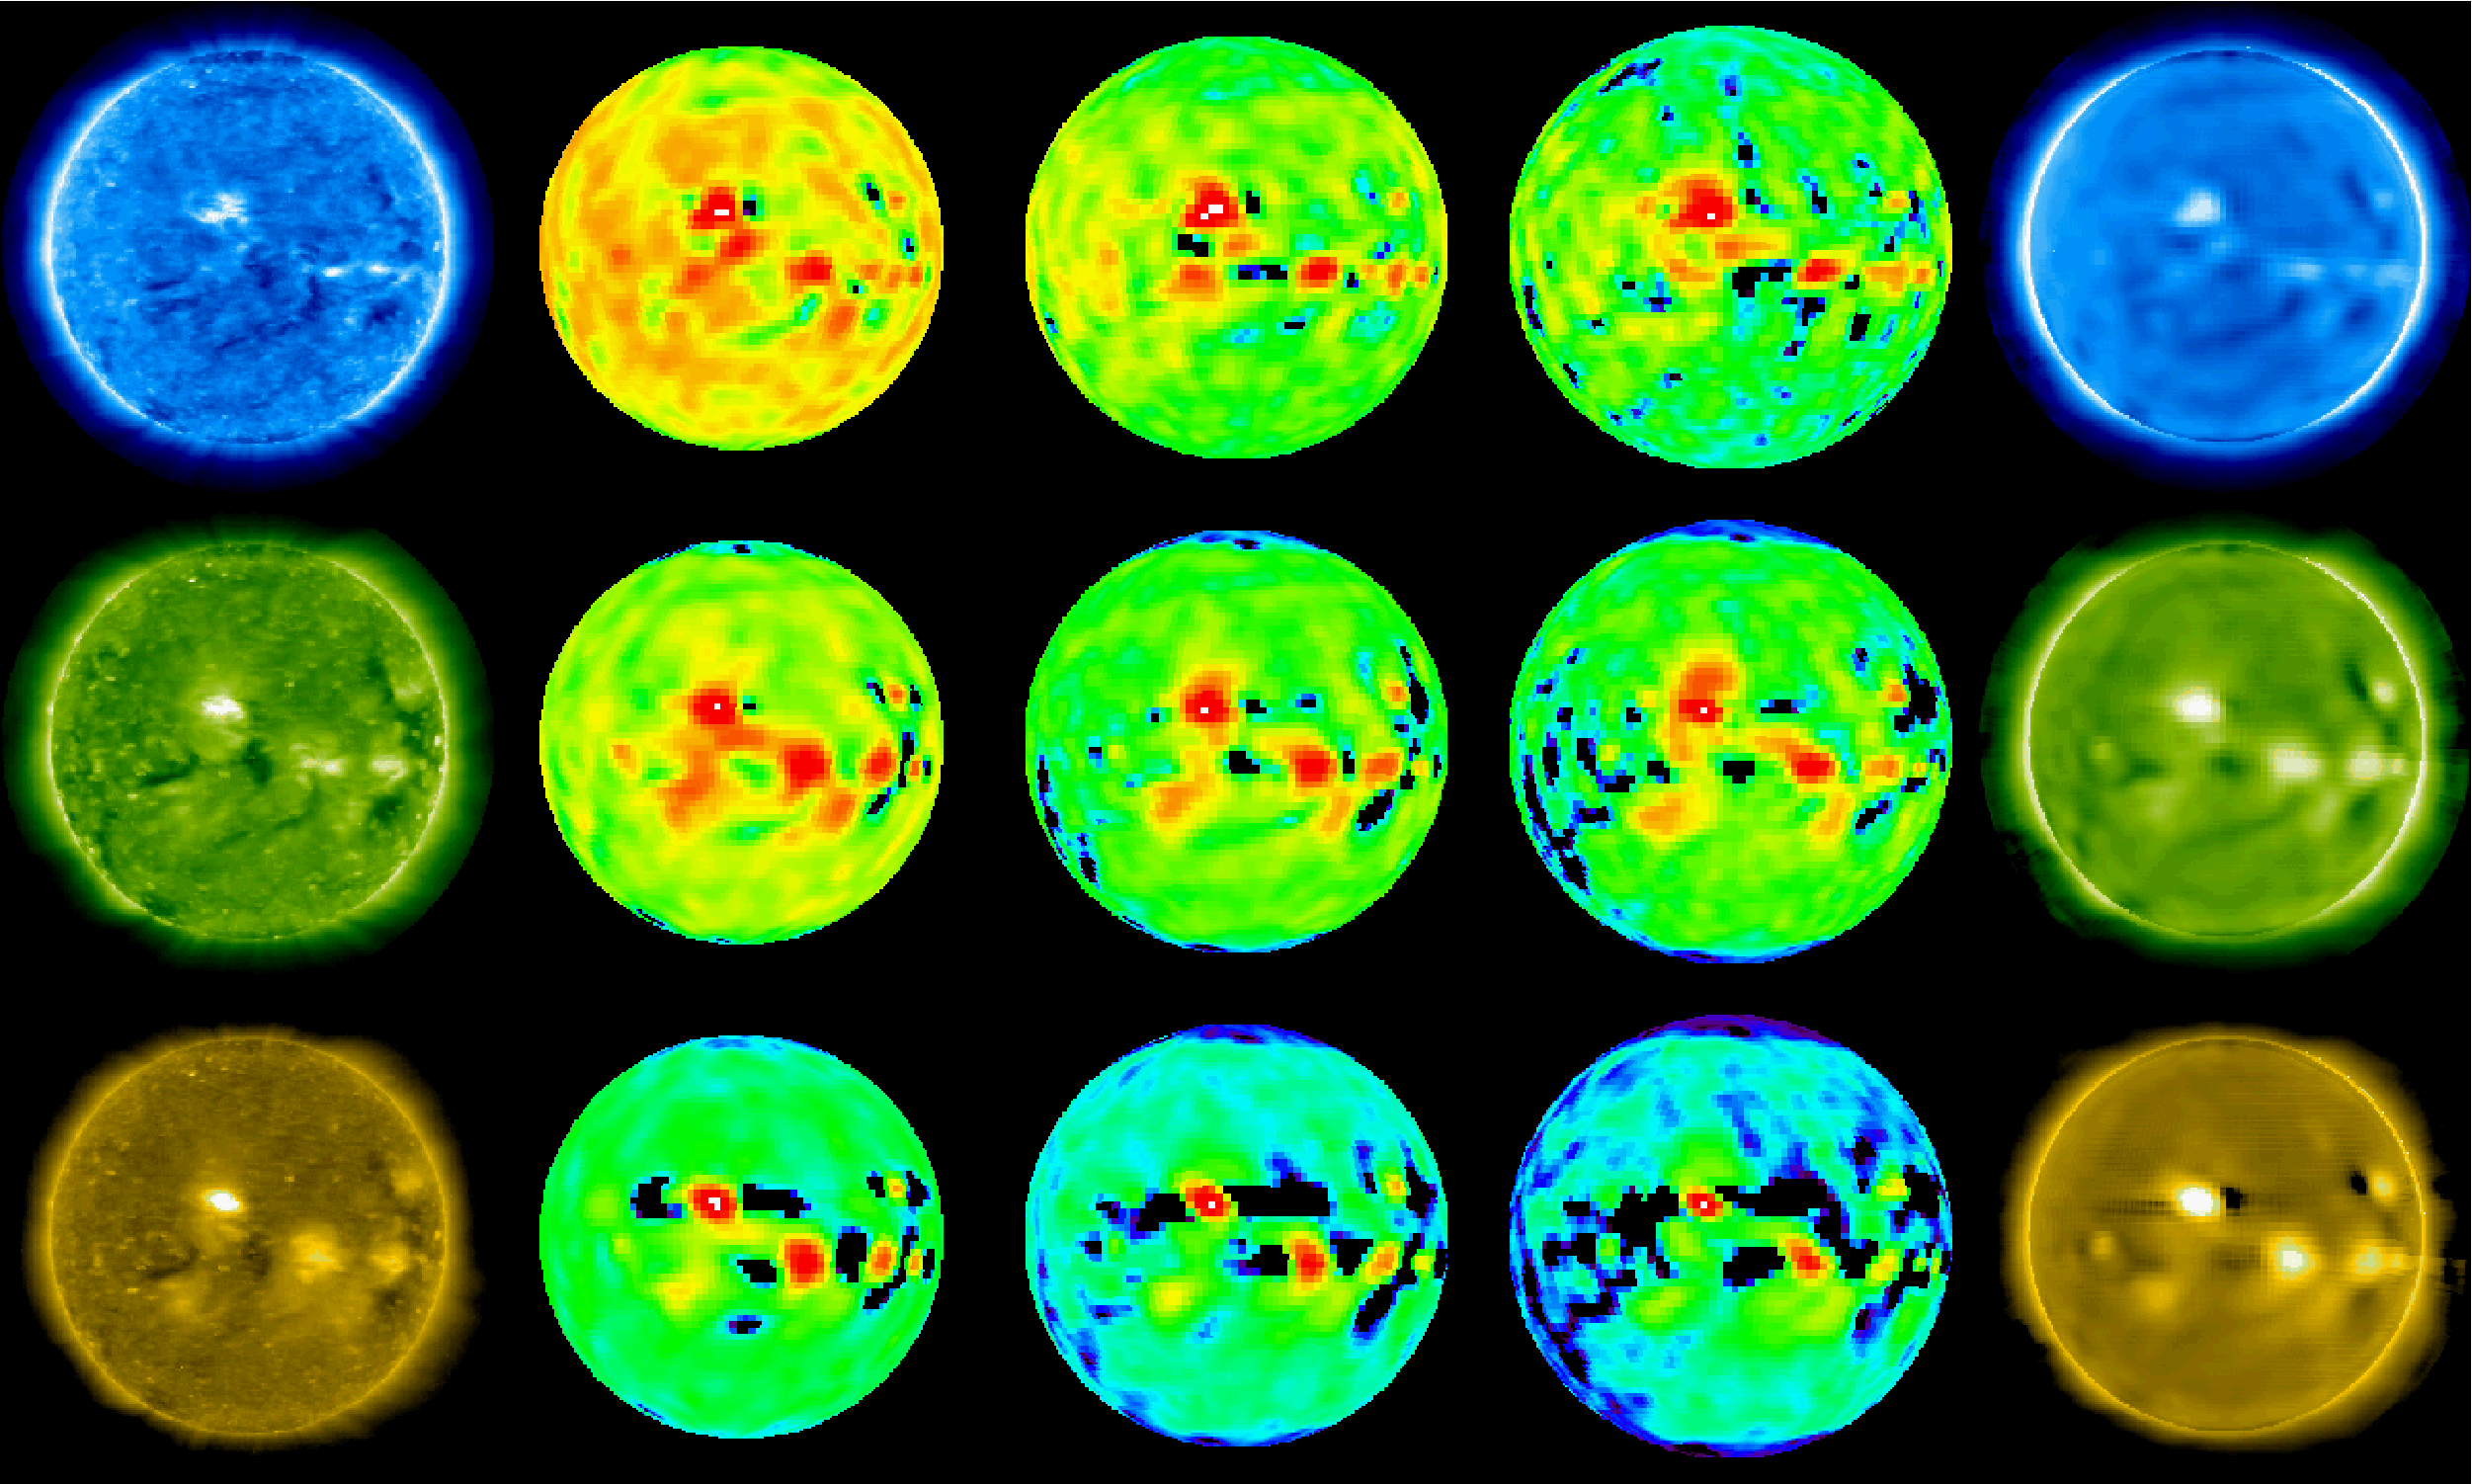
\includegraphics[width=0.95\linewidth]{figuras/frame_050_test.pdf}}\\
\footnotesize
 1.035 $\mrsun$ \hskip 1cm 1.085 $\mrsun$ \hskip 1cm 1.135 $\mrsun$ \hfil
\end{center}
\end{columns}
\begin{columns}
 \column{0.4\textwidth}
 Vásquez et al. (2009)
 \column{0.6\textwidth}
\end{columns}
}
\end{comment}
%----------------------------------- LDEM

\frame{
\titulo{The Local Differential Emission Measure (LDEM)}
\footnotesize
\begin{itemize}
\item[\bu]
For each band \azul{$k$} we know now the FBE {$\azul{E_{k,i}}$} at each tomographic cell \azul{$i$}.
\salto
\item[\bu]
Using the temperature responses $\azul{Q_k(T)} \equiv \int {\rm d} \lambda \ \phi_k(\lambda) \ {\eta( N_{e0}, {\bf a}_0,
T; \lambda)}  /  {N_{e0}^2}$
\salto
\item[\bu]
The FBEs can be re-written as:
$\azul{FBE_{k,i} } \, = \, \azul{\int \mathrm{d}T \  Q_k(T) \ \, \rojo{{\sf LDEM}_i(T)} }$.
\salto
\item[\bu]
%Donde la \rojo{${\sf LDEM}_i(T)$ [cm$^{-6}$K$^{-1}$]} para cada celda \azul{$i$} se define tal que:
The \rojo{${\sf LDEM}_i(T)$ [cm$^{-6}$K$^{-1}$]} of each cell \azul{$i$} is defined so that:
\begin{eqnarray}
N_{m,i}^2 = \left< N_e^2\right>_i &=& \int \mathrm{d} T \ \, \rojo{{\sf LDEM}_i(T)}\nonumber\\
T_{m,i} = \left<T_e\right>_i  &=& \frac{1}{\left< N_e^2\right>_i } \int \mathrm{d}T\ T \ \, \rojo{{\sf LDEM}_i(T)}\nonumber \\
 W_{T,i}^2 &=&  \frac{1}{\left< N_e^2\right>_i} \int_{T_{min}}^{T_{max}} dT\ \rojo{{\sf LDEM}_i(T)}\ (T - \langle T_e \rangle_i)^2 \nonumber
\end{eqnarray}
%\salto
\item[\bu] Parametric model for the LDEM:\ 
$\rojo{{\sf LDEM}_i(T)}=\azul{\mathcal{N}(}T,\,\rojo{\mathbf{\lambda}_i=[A,T_0,\sigma_T]}\azul{)}$ 
\salto
\item[\bu]
The following objective function is minimized in each cell: \mediosalto
\hskip 3cm
$
\Phi(\rojo{{\mathbf{\lambda}}_i}) \ = \ 
\ \azul{\sum_{k}}| \ \azul{ FBE_{k,i} }-
\azul{\int \mathrm{d}T \ \, Q_k(T)\ \, \mathcal{N}(T,}\,\rojo{\mathbf{\lambda}_i}\azul{)} \ 
|^2 
$.
\item[\bu] Success rate
$
R_i \equiv (1/K) \sum_{k} | 1 - { FBE_{k,i} } / {\int \mathrm{d}T \ \, Q_k(T)\ \, \mathcal{N}(T,}\,{\mathbf{\lambda}_i}{)} |
$
\end{itemize}
}


%--------------------------
\frame{
\titulo{LDEM}

\begin{columns}
\column{0.5\textwidth}
%Lloveras et al. (2022)
\begin{center}
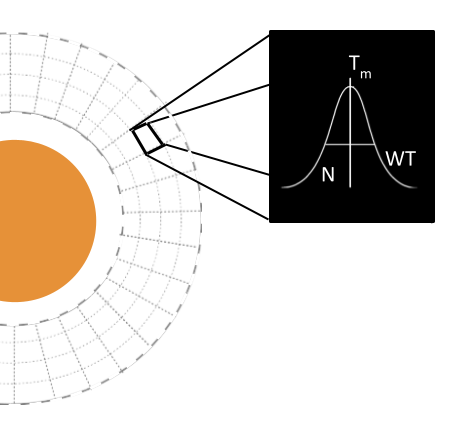
\includegraphics[height=0.6\textwidth]{figuras/Grid_LDEM.png}
\end{center}
\column{0.5\textwidth}
%\begin{itemize}
%\item[\bu] \small{$R_i \equiv (1/K) \sum_{k} | 1 - { FBE_{k,i} } / { SYN_{k,i} }|$}
%\item[\bu] \small{$R_i \equiv (1/K) \sum_{k} | 1 - { FBE_{k,i} } / {\int \mathrm{d}T \ \, Q_k(T)\ \, \mathcal{N}(T,}\,{\mathbf{\lambda}_i}{)} |$}
%\end{itemize}
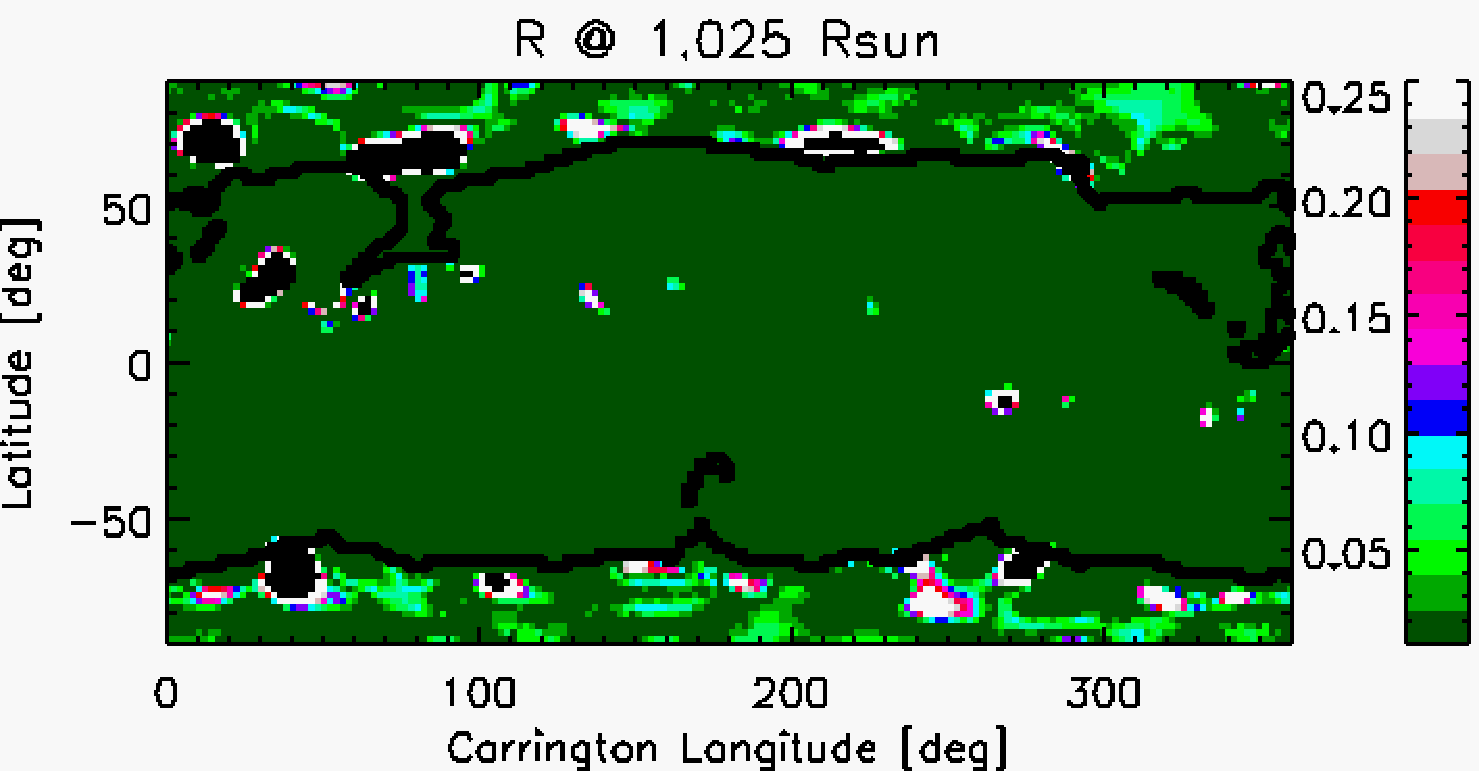
\includegraphics[width=0.9\textwidth,clip=]{figuras/R_1025_CR2081.pdf}
%\hfill Lloveras et al. (2022)\\
%\vskip 2cm
\begin{itemize}
\item[\bu] \small{$R \sim 1\% \, (Str.) \, y \sim 10\% \, (CHs)$}
\end{itemize}
%\hfill Lloveras et al. (2022)\\
\end{columns}


\begin{center}
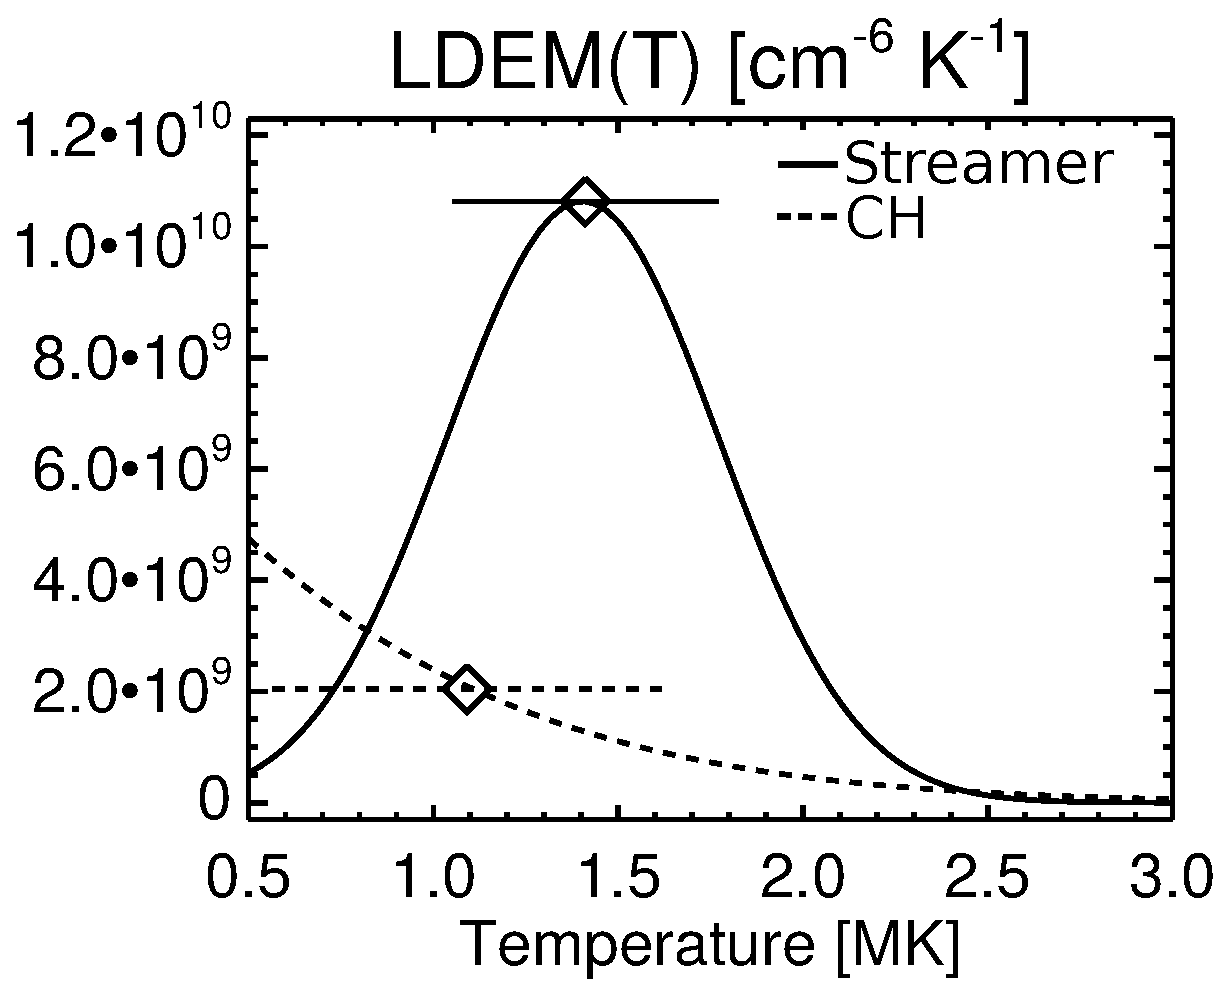
\includegraphics[width=0.4\textwidth,clip=]{figuras/Nueva_figura_paper_LDEM_2.eps}
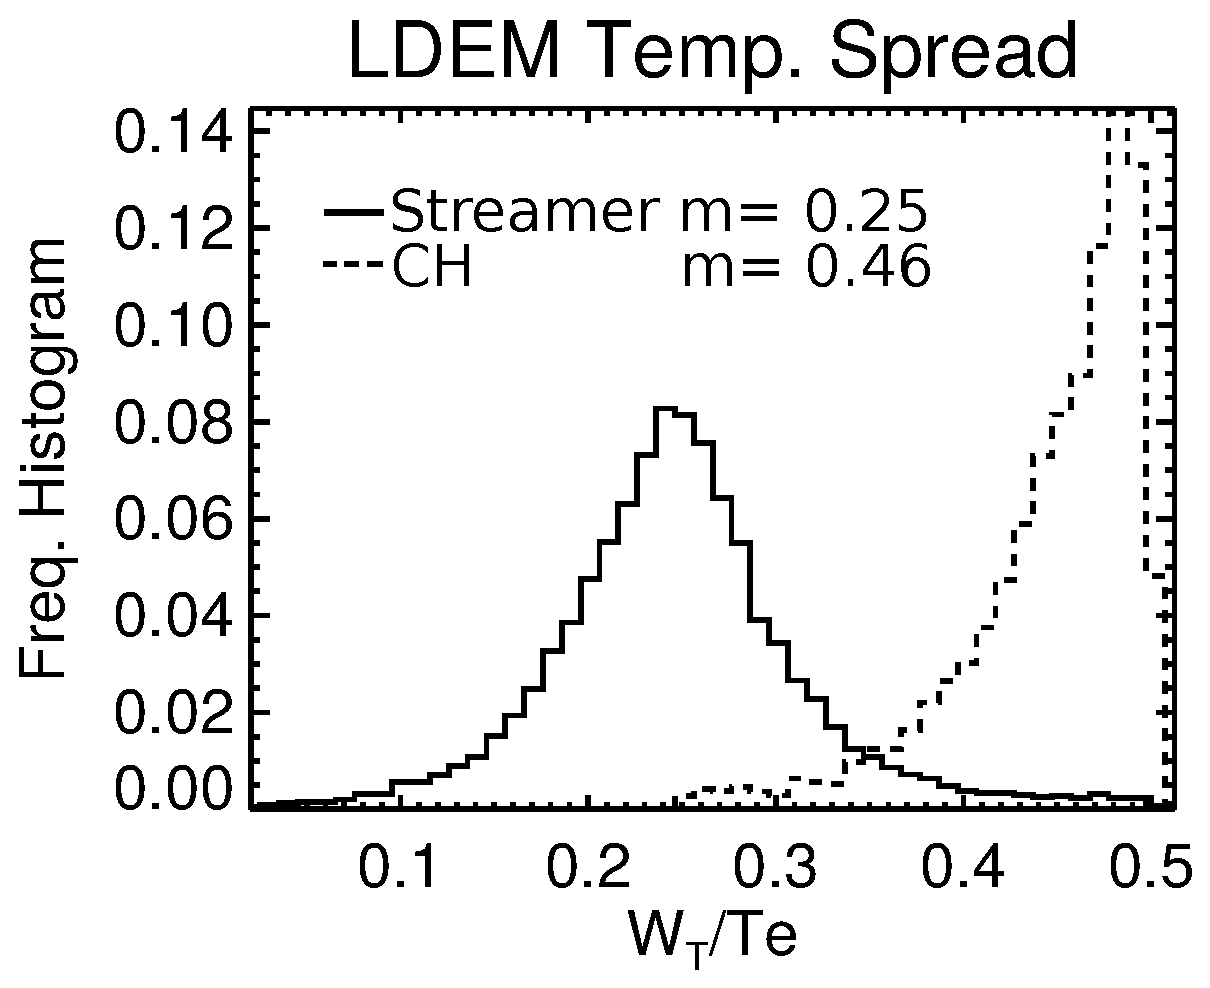
\includegraphics[width=0.4\textwidth,clip=]{figuras/Nueva_figura_paper_3.eps}
\end{center}
}

%--------------------------------------------
\frame{
\titulo{DEMT Validation of {\sc awsom}: Coronal Base}
\footnotesize
%\begin{columns}
%\column{0.7\textwidth}
\begin{center}
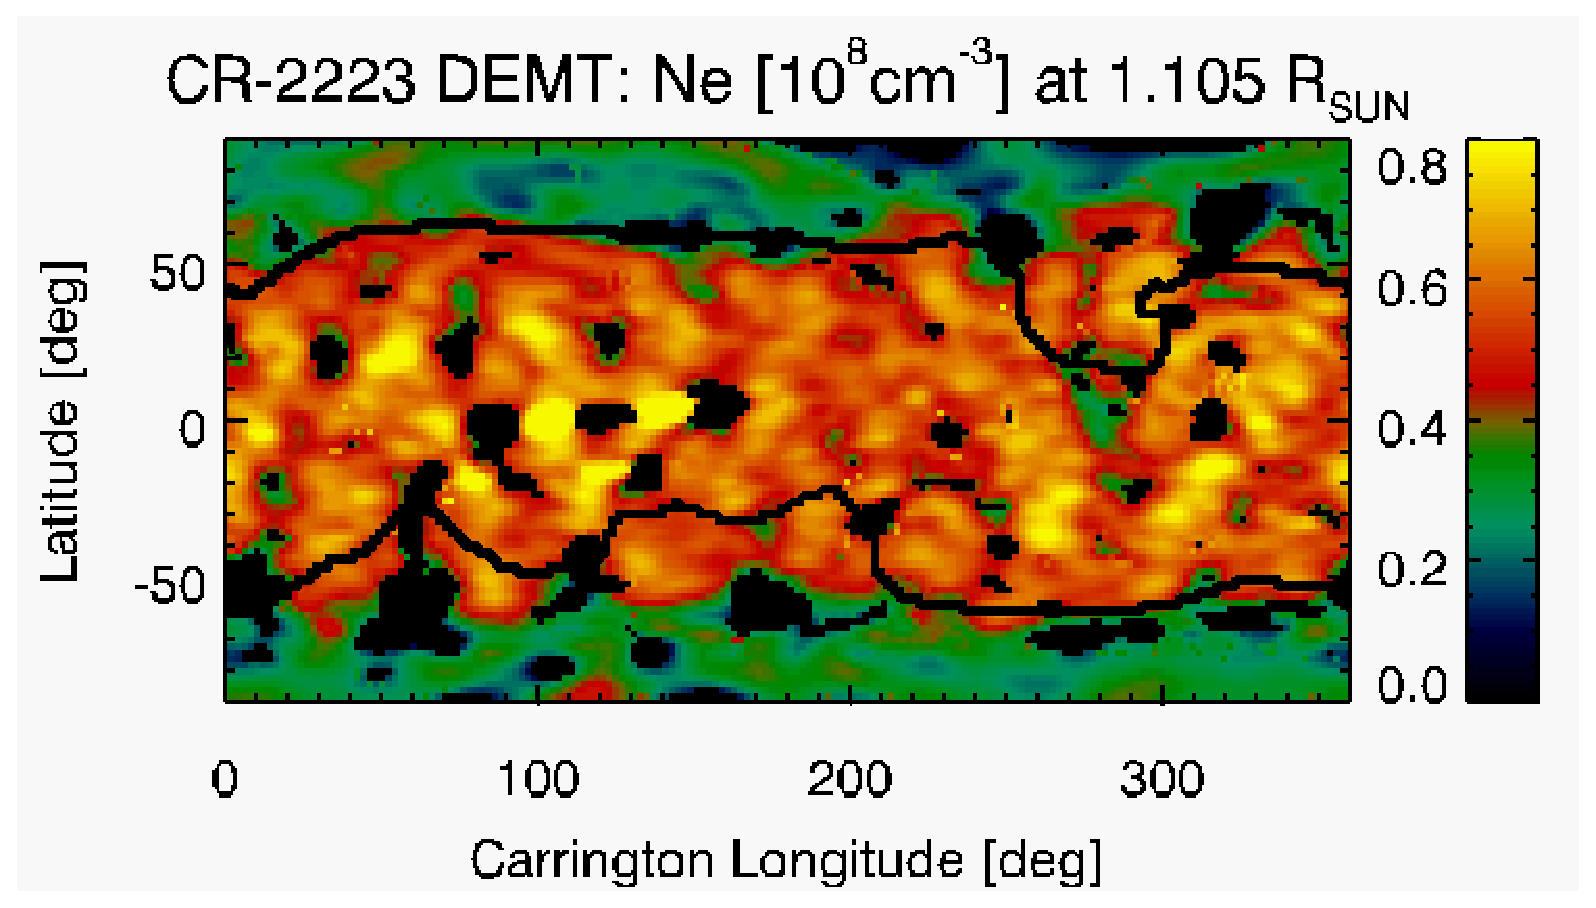
\includegraphics[width=0.49\textwidth,clip=]{figuras/map_Ne_CR2223_DEMT-AIA_H1_L733_r3d_multistart_1105_Rsun2223.eps}
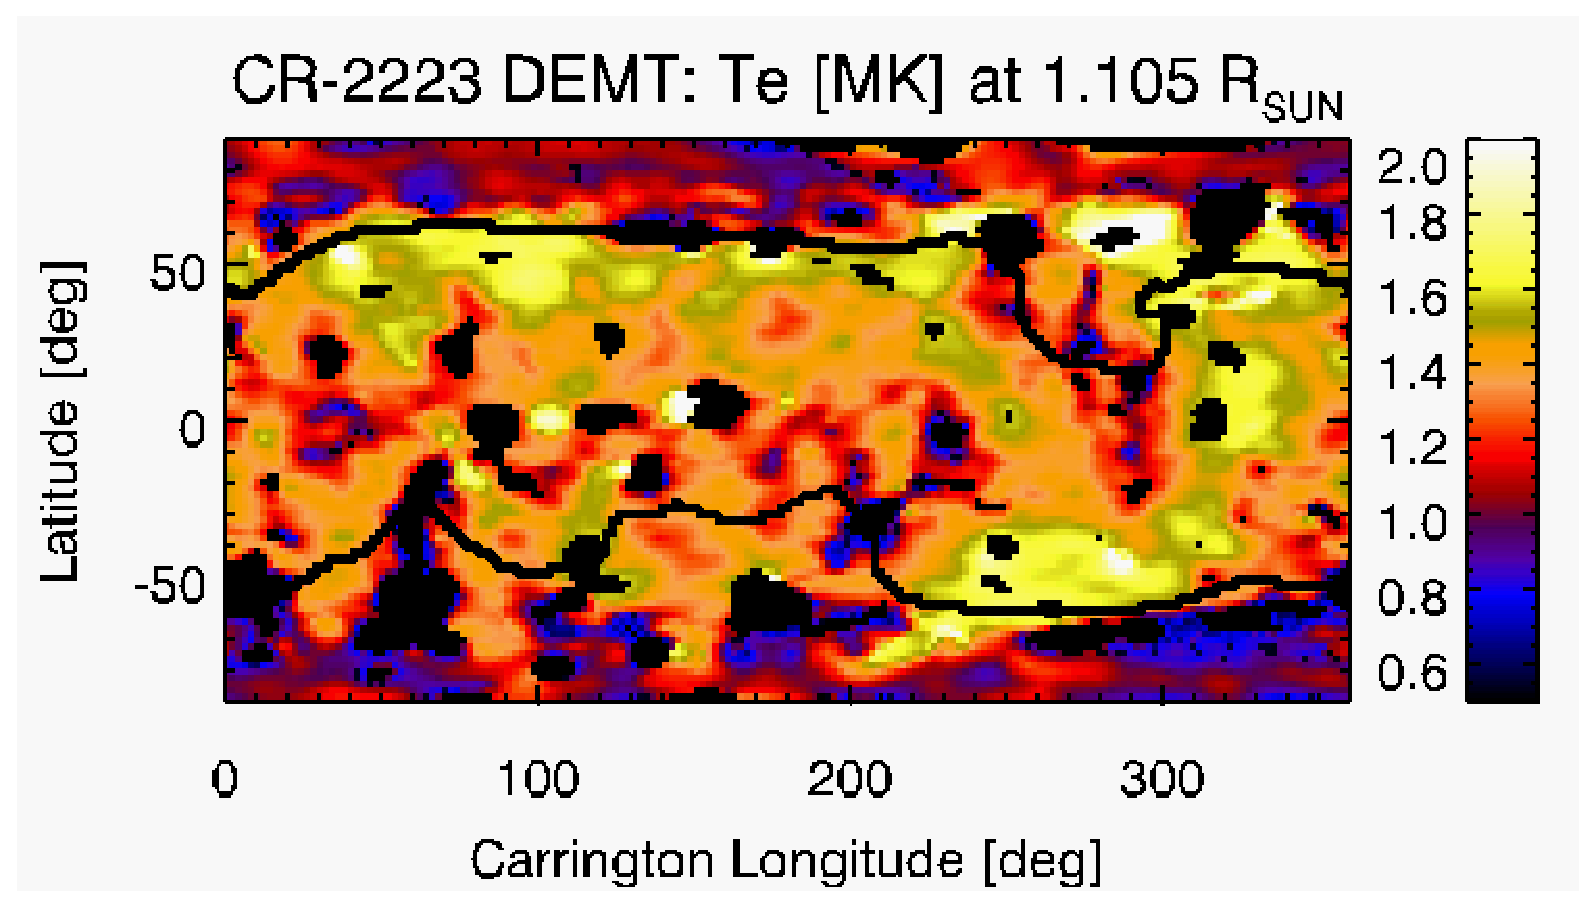
\includegraphics[width=0.49\textwidth,clip=]{figuras/map_Tm_CR2223_DEMT-AIA_H1_L733_r3d_multistart_1105_Rsun2223_2.eps}
\vskip 0.25cm
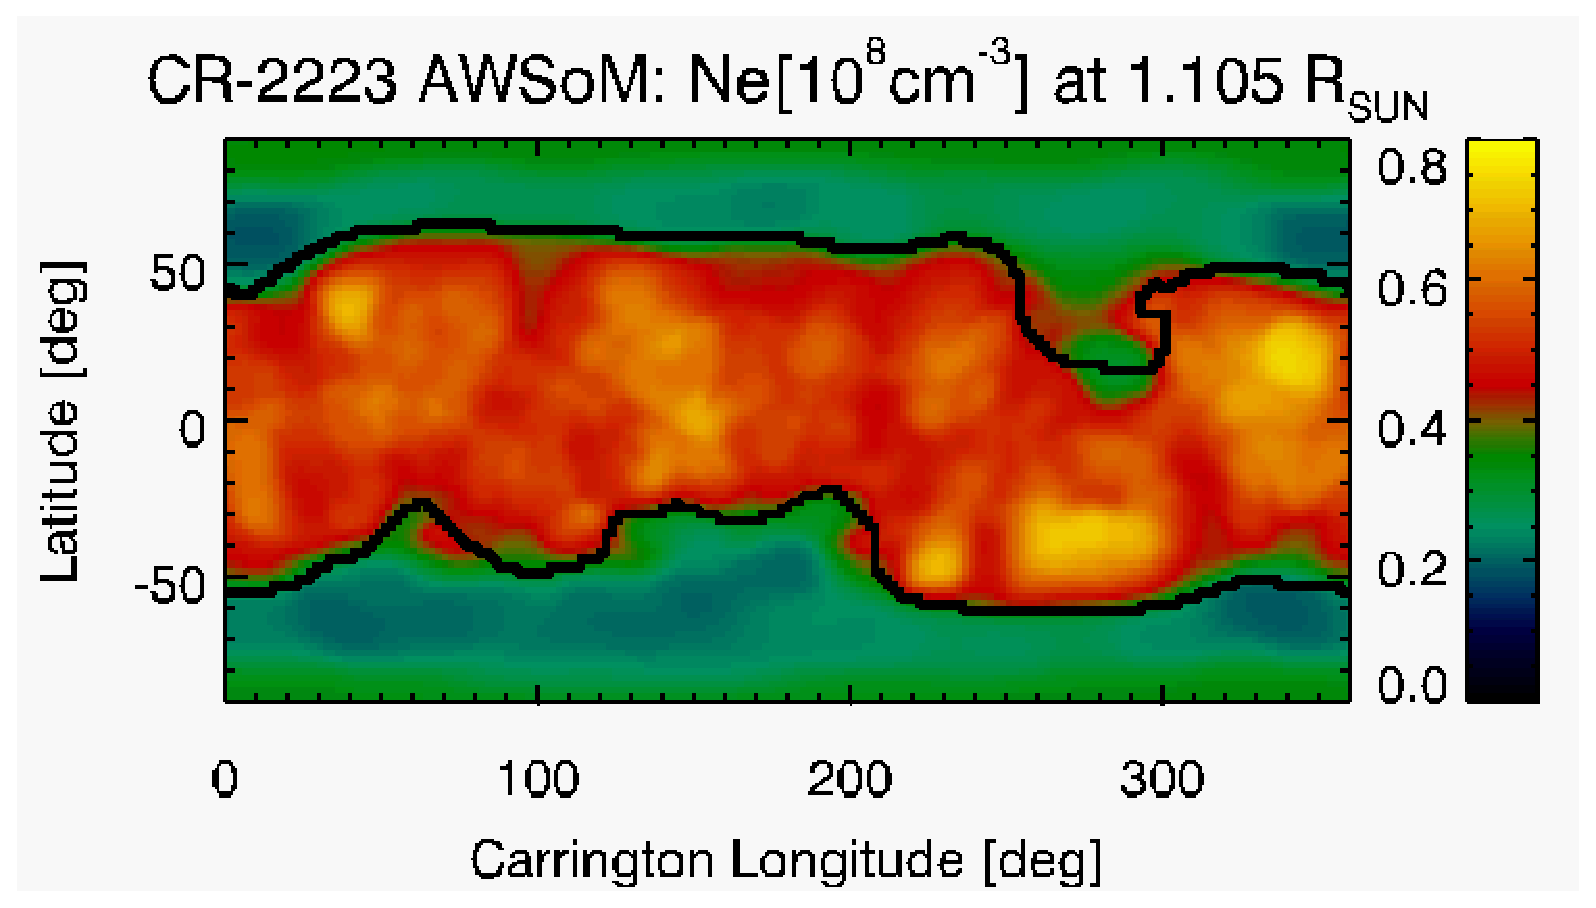
\includegraphics[width=0.49\textwidth,clip=]{figuras/map_Ne_awsom_2223_ener_new_1105_Rsun2223.eps}
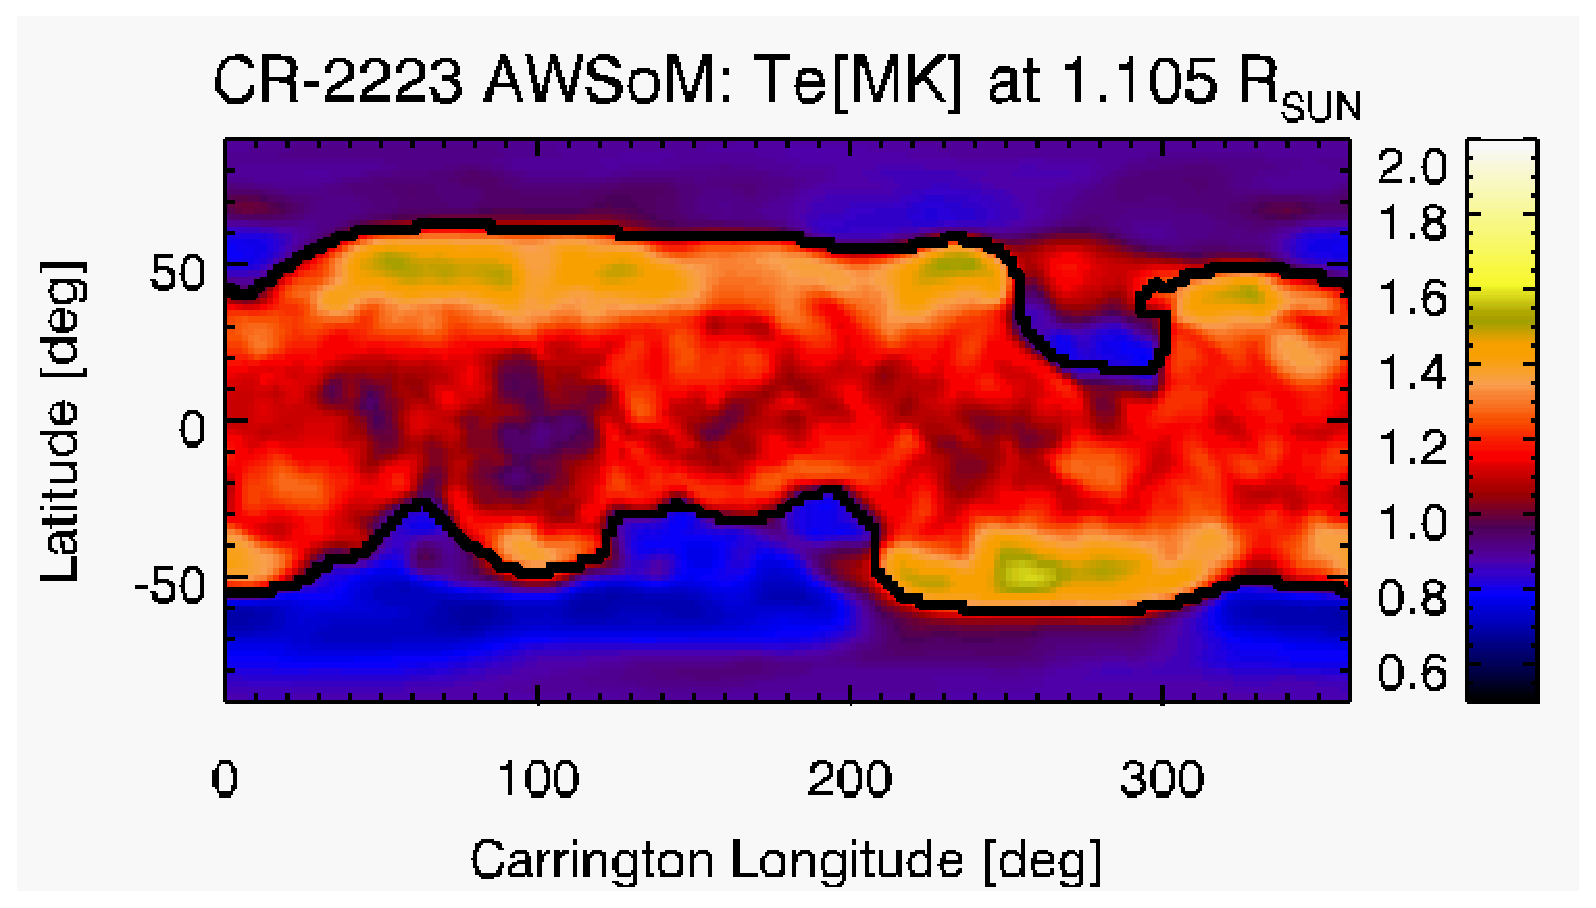
\includegraphics[width=0.49\textwidth,clip=]{figuras/map_Te_awsom_2223_ener_new_1105_Rsun2223_2.eps}
\vskip 0.25cm
%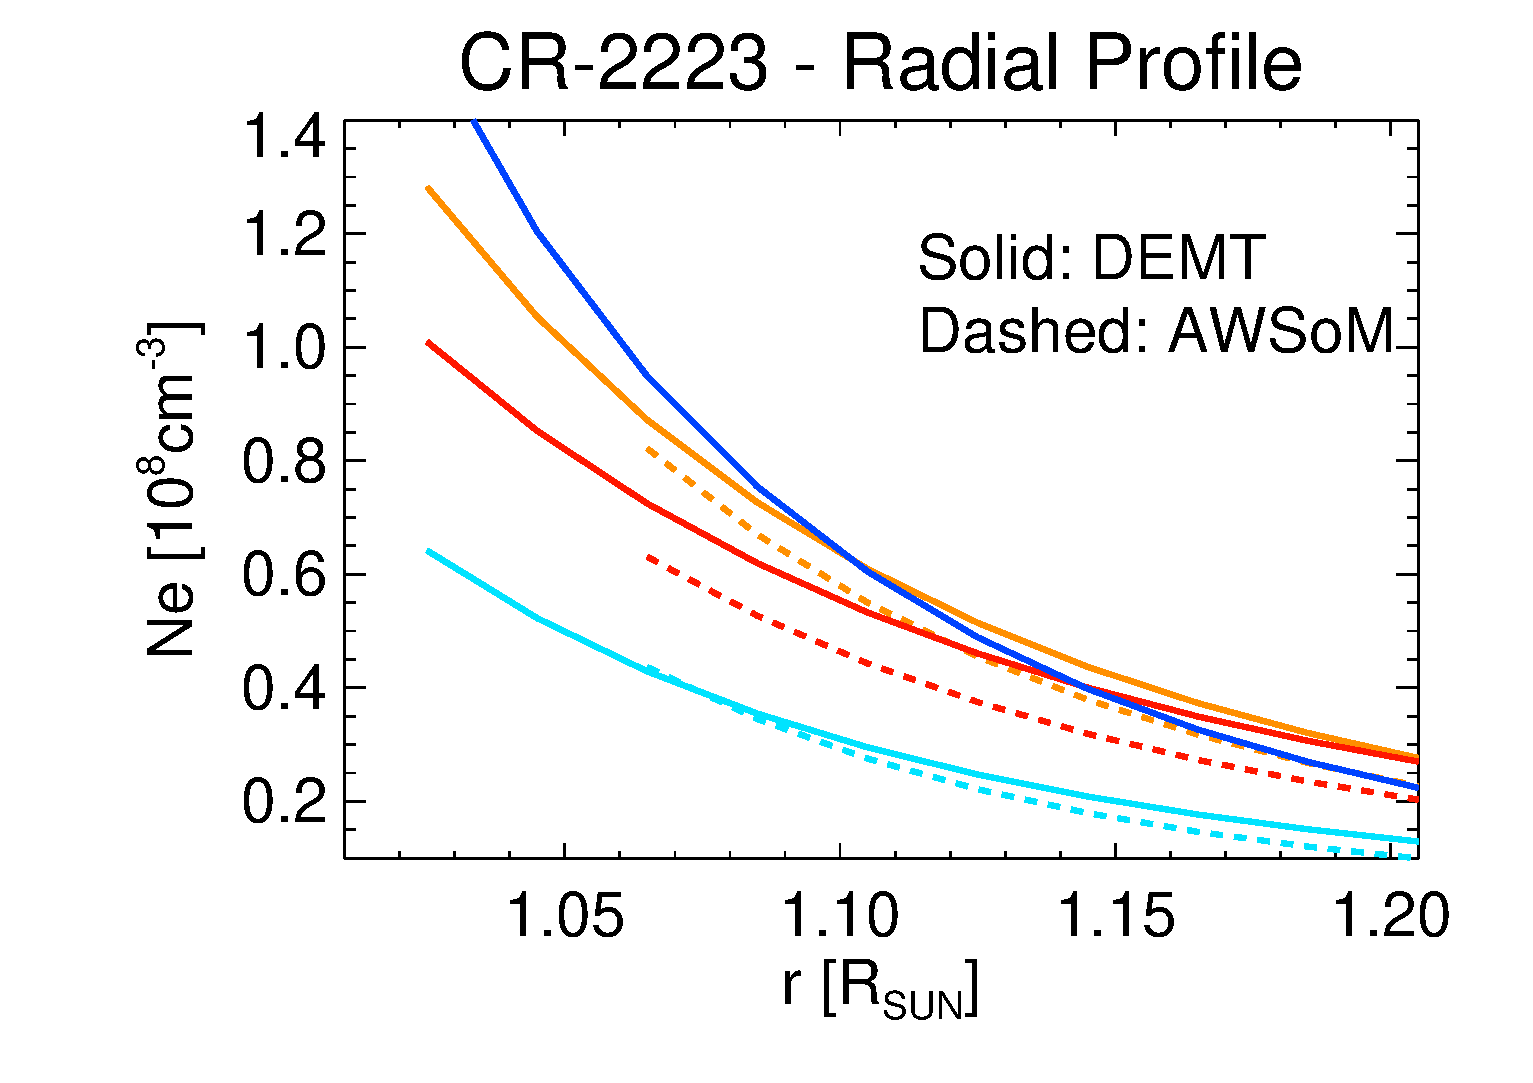
\includegraphics[width=0.49\textwidth,clip=]{figuras/perfil_paper_necr2223_bajo.eps}
%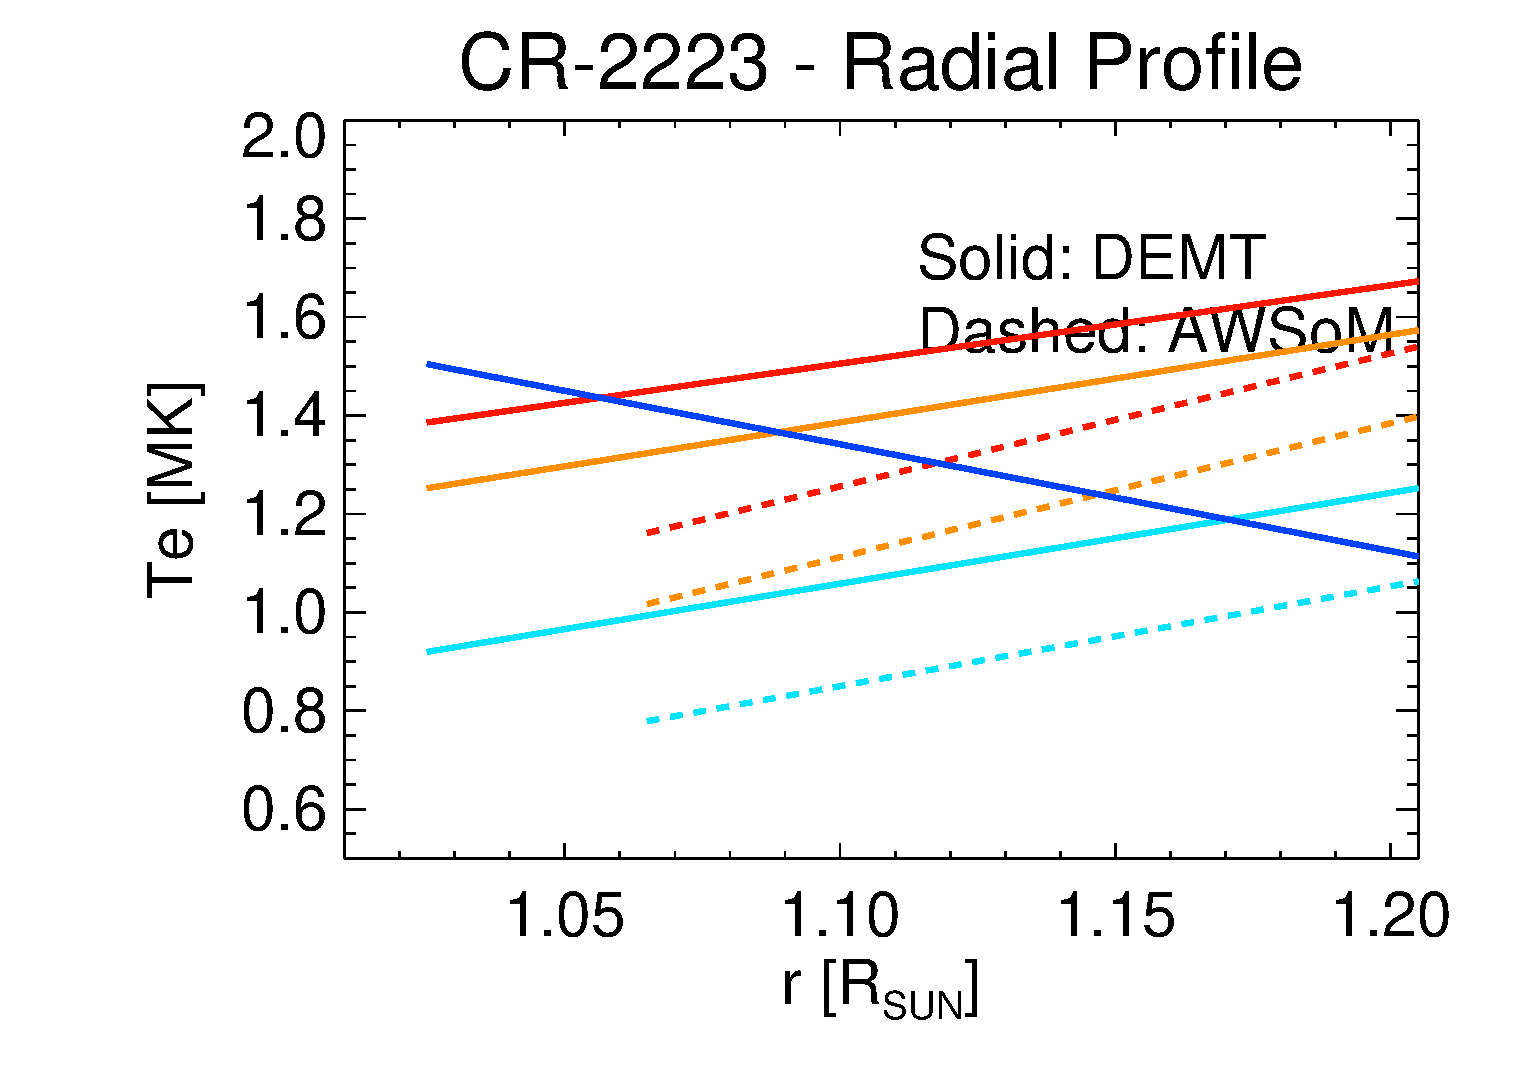
\includegraphics[width=0.49\textwidth,clip=]{figuras/perfil_paper_tecr2223_bajo.eps}
\vspace{-0.05cm}

\end{center}
%\column{0.3\textwidth}
%\bu Analysis of campaigns of Whole Heliosphere and Planetary Interactions (WHPI).
%\vskip 0.5cm
\begin{columns}
\column{0.5\textwidth}
%\bu Consistent North O/C and CH.\\
%\vskip 0.5cm
\bu Good consistency, in terms of shape and size of the streamer belt and the CHs.\\
%\vskip 1.5cm
\column{0.5\textwidth}
%\bu $\Delta\Ne(r) \approx \pm 5\%$.\\
%\vskip 0.5cm
%\bu $\Delta\Te(r) \approx -15\%$.\\
%\vskip 0.5cm
\bu Southern O/C shifted $\approx +20^\circ$ from CH.\\
\hfill van der Holst et al (2014)
\end{columns}
}



%--------------- imág sintéticas
\frame{
\titulo{EUV Synthetic Images: SRT vs. {\sc awsom}}
\begin{center}
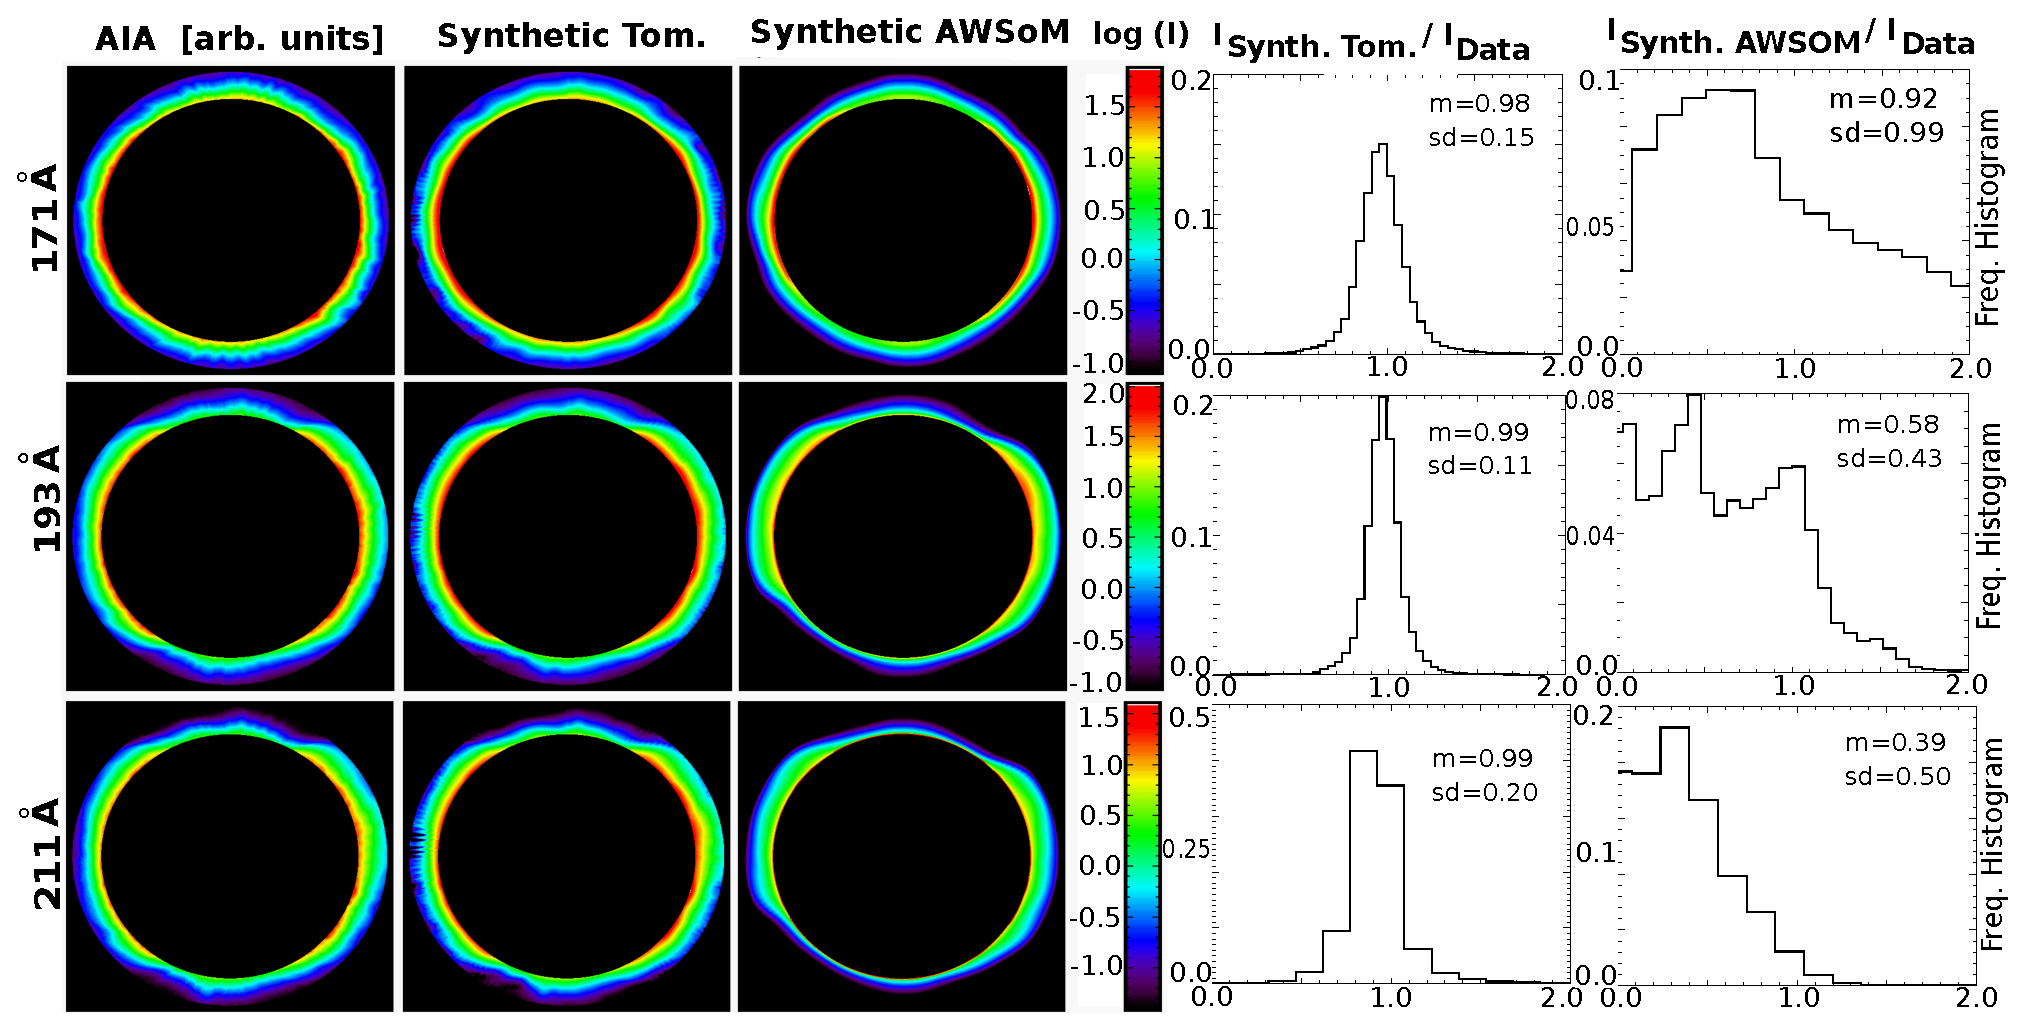
\includegraphics[width=0.99\textwidth,clip=]{figuras/Figura_2_paper_imag_sinteticas_2.eps}
\end{center}
$I_{Synt} \sim \int_{LOS} \mathrm{d}l \, N_e^2 \, Q_k$\\
\vskip 0.2cm
%\begin{itemize}
  %\item[\bu] 
\bu {\sc awsom} O/C discrepancy due to lack of accuracy of boundary condition.$ \rightarrow$
ADAPT-GONG not able to reproduce the large-scale structure of the CH boundary in this specific region.
%\end{itemize}
}


%-----------------------
\frame{
\titulo{Tomographic Results along {\bf B}-lines}
\footnotesize
%\begin{columns}
%\column{0.5\textwidth}
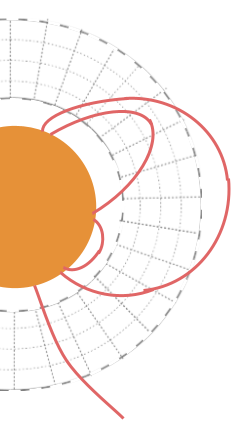
\includegraphics[height=0.35\linewidth]{figuras/Grid-loops.png}
\includegraphics[height=0.35\linewidth]{figuras/Traced-Loop.eps}
%\column{0.5\textwidth}
%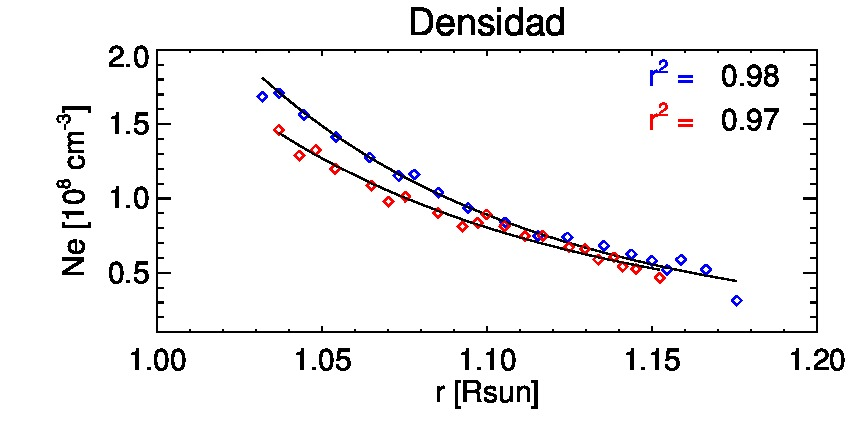
\includegraphics[width=0.8\textwidth]{figuras/loop_Ne2.jpg}
%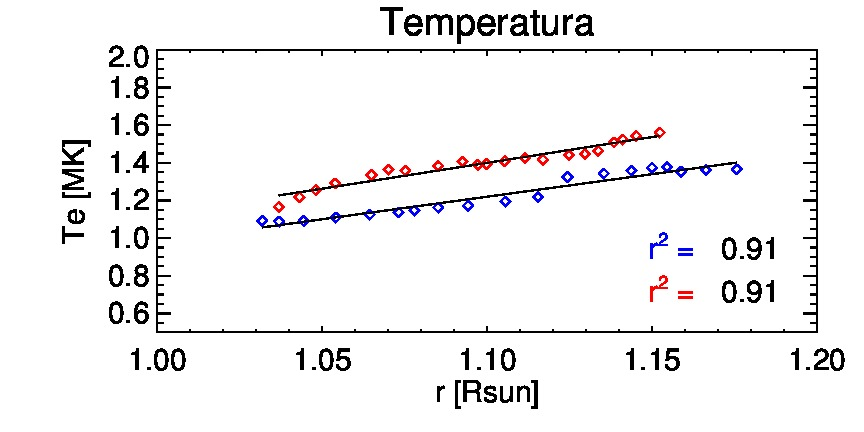
\includegraphics[width=0.8\textwidth]{figuras/loop_T2.jpg}
%\end{columns}
%\begin{center}
\salto
\begin{columns}
\column{0.5\textwidth}
Results along individual {\bf B}-lines are characterized by parametric fits:
%\begin{eqnarray*}
%\Ne(h) &=& N_0\ \textsf{exp}\left(-h/\lambda\right)
$ N_e = N_0\, \exp{[-(h/\l)/(r/\mrsun)]}$\\
$ T_m = ar + b$\\
%\\
%\Te(h) &=& T_0 \, + \, \gamma \, h
%$$\hfill \ \ \ \ \ \ \ \ T_m = ar + b$$
%\end{eqnarray*}
and fitting parameters are analyzed statistically.\\
\rojo{UP} \, \, \,  $(a \equiv \dTm_dr>0)$\\
\azul{DOWN} $(a \equiv \dTm_dr<0)$
\column{0.5\textwidth}
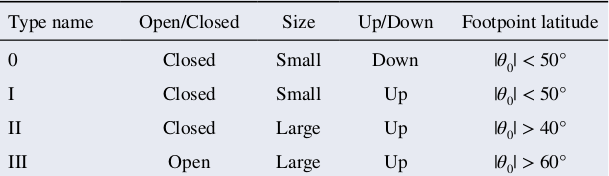
\includegraphics[width=0.99\textwidth]{figuras/tabla1_paper.png}
\end{columns}
%\end{center}
}
%----------------Trazado - Ajuste DEMT

\frame{
\titulo{Position of traced magnetic field lines}
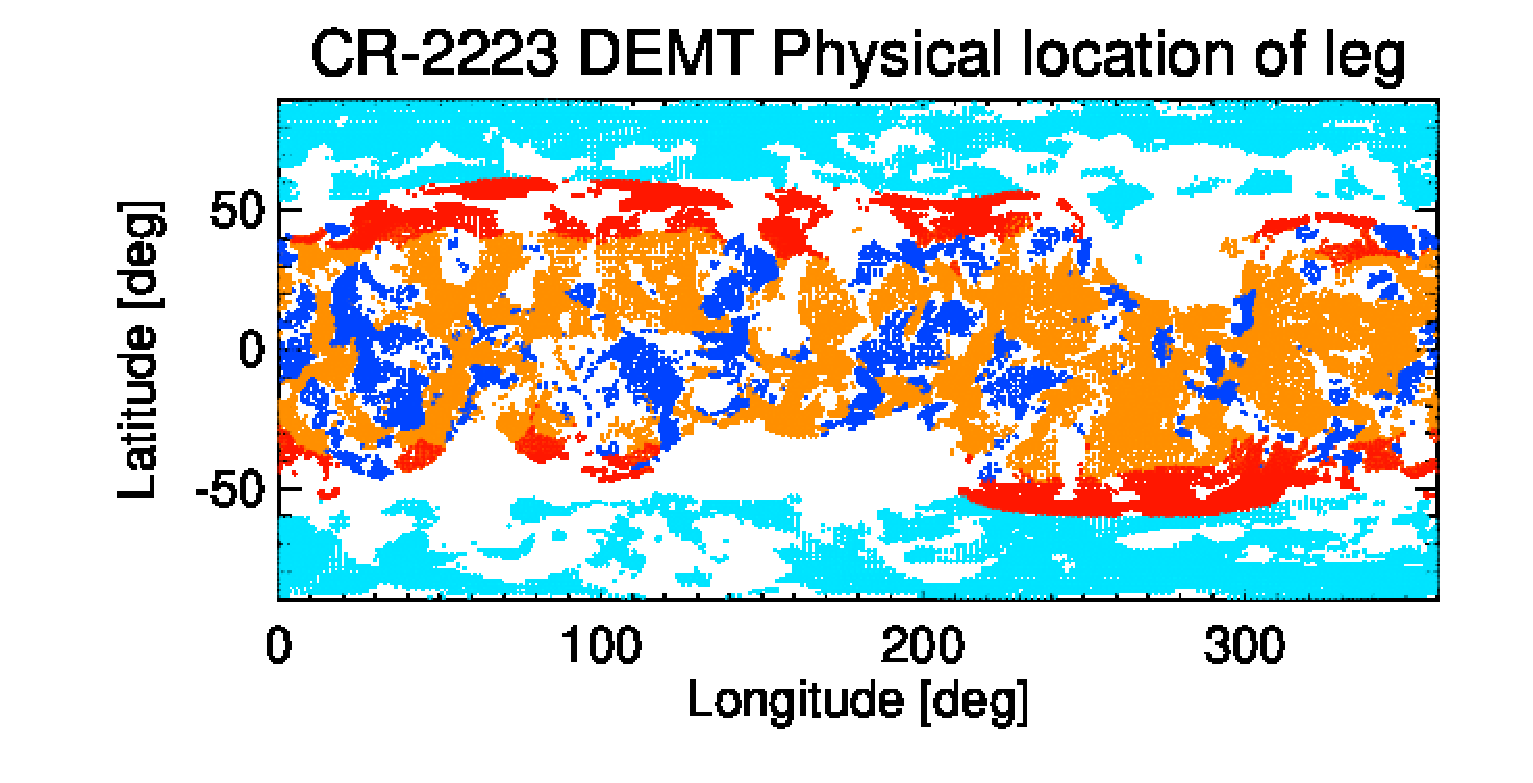
\includegraphics[width=0.49\textwidth,clip=]{figuras/Highpoint_2223_demt_BAJO_Rpoint-map_2.eps}
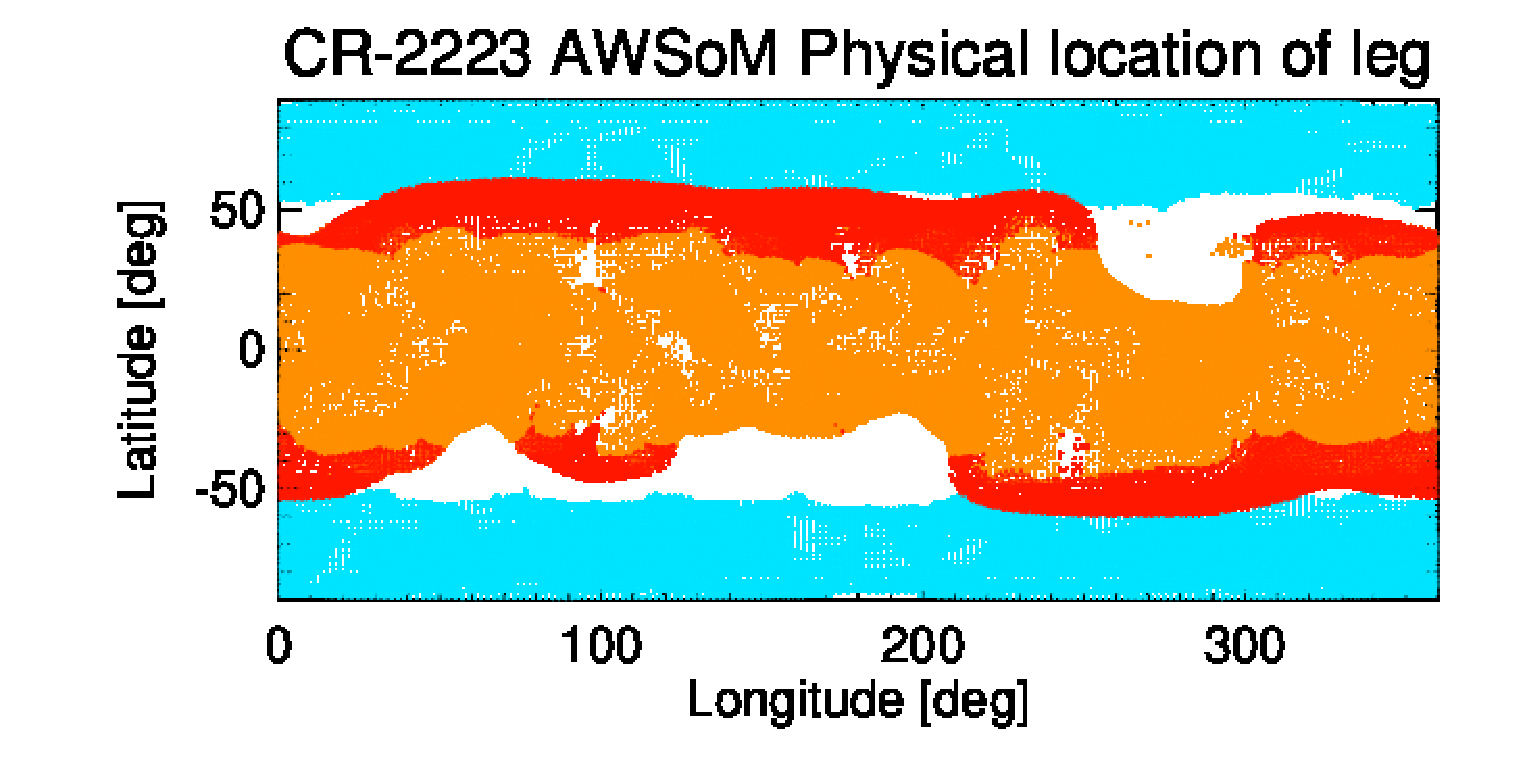
\includegraphics[width=0.49\textwidth,clip=]{figuras/Highpoint_2223_awsom_BAJO_Rpoint-map_2.eps}\\
%\begin{columns}
%\column{0.33\textwidth}
%\footnotesize
\centering
\begin{tabular}{c c c }
\hline
  Type  & Characteristic     \\
\hline
   0   & \azul{Closed Small Down}   \\
   I   & \orange{Closed Small Up}   \\
   II  & \rojo{Closed Large Up}     \\
   III & \cian{Open Large Up}    \\
\hline
\end{tabular}
%\column{0.33\textwidth}
%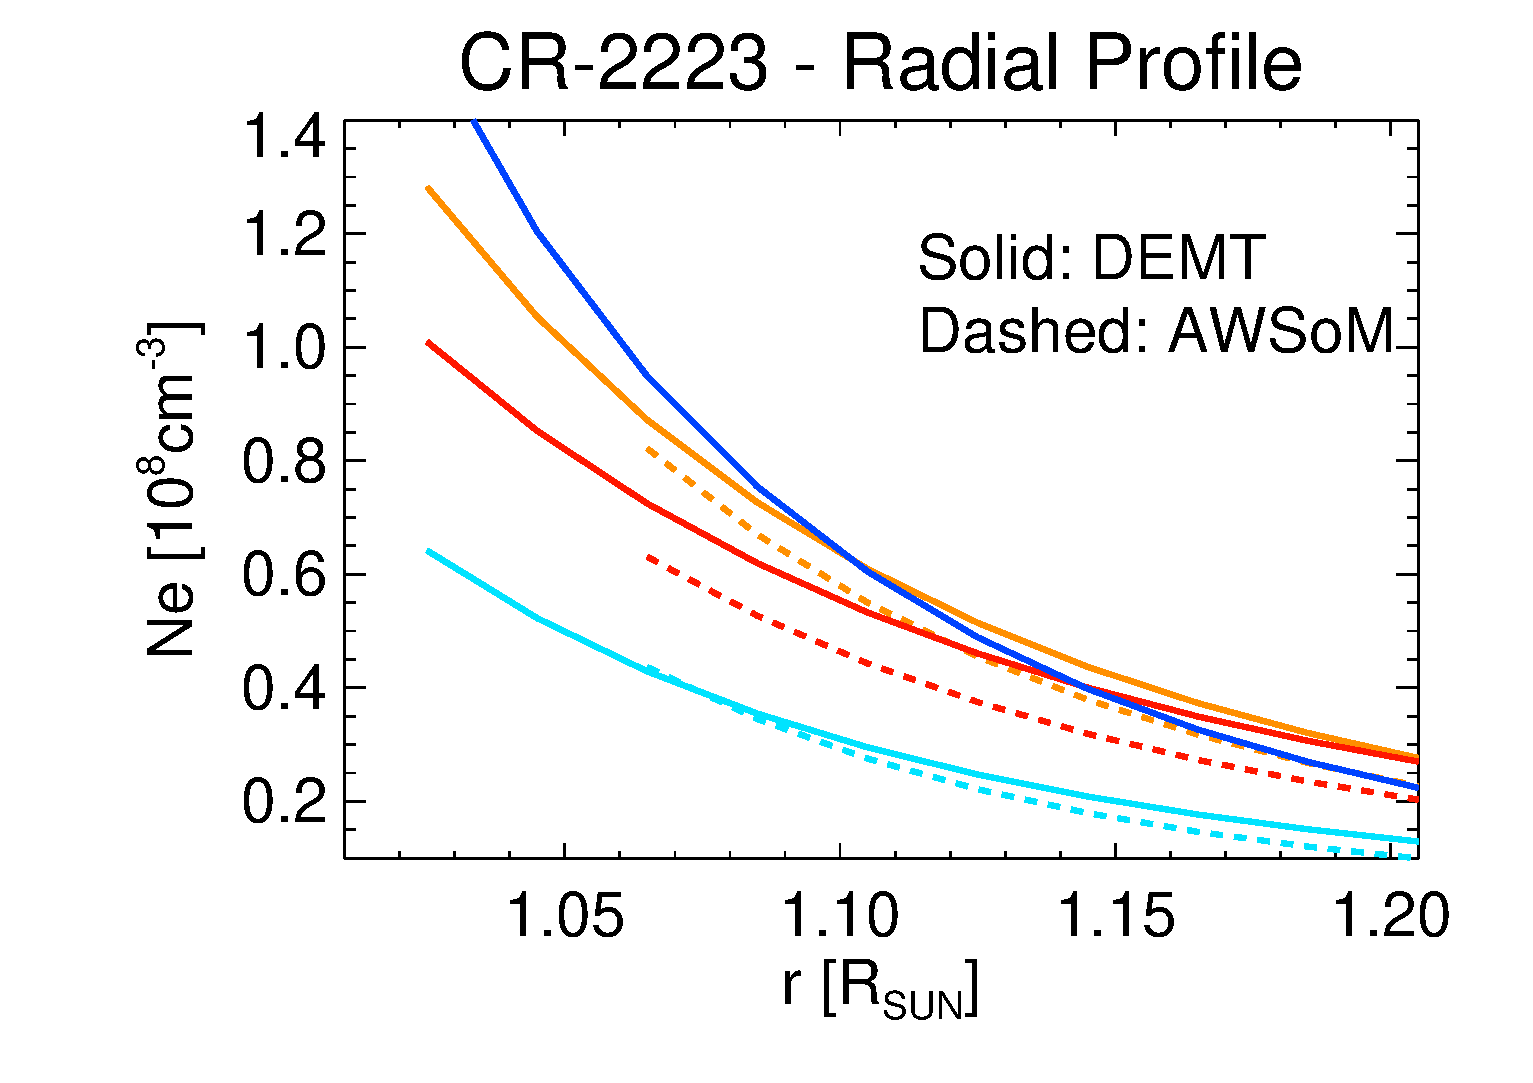
\includegraphics[width=0.99\textwidth,clip=]{figuras/perfil_paper_necr2223_bajo.eps}
%\footnotesize
%\bu Streamer (T0 $\rightarrow$ TII):\\
%$N_{CB}$ decrease; $\lambda_N$ y $\left<T_m\right>$ increases. \\
%\column{0.33\textwidth}
%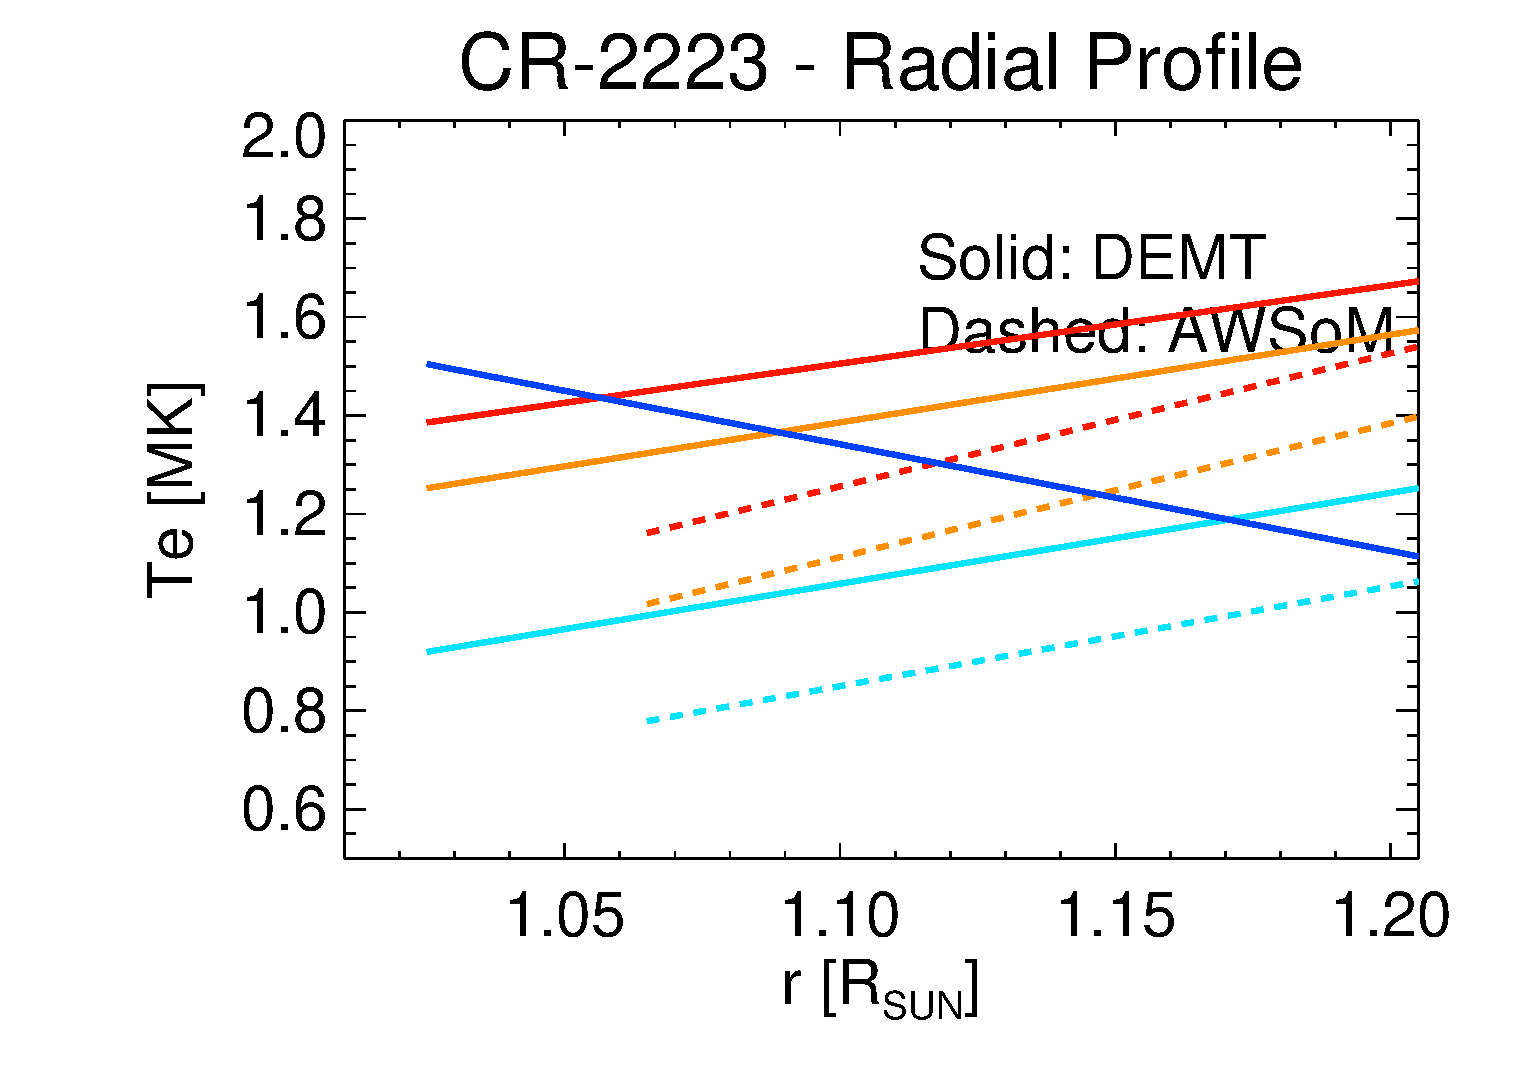
\includegraphics[width=0.99\textwidth,clip=]{figuras/perfil_paper_tecr2223_bajo.eps}
%\footnotesize
%\bu CHs (T III): \\
%$N_{CB}$, $\lambda_N$ y $\left<T_m\right>$ decrease.\\
%\end{columns}
%\bu $\Delta\Ne(r) \approx \pm 5\%$.
%\bu $\Delta\Te(r) \approx -15\%$.\\
}
%-------------------------------------


\frame{
\titulo{Average fits}
\begin{columns}
\column{0.5\textwidth}
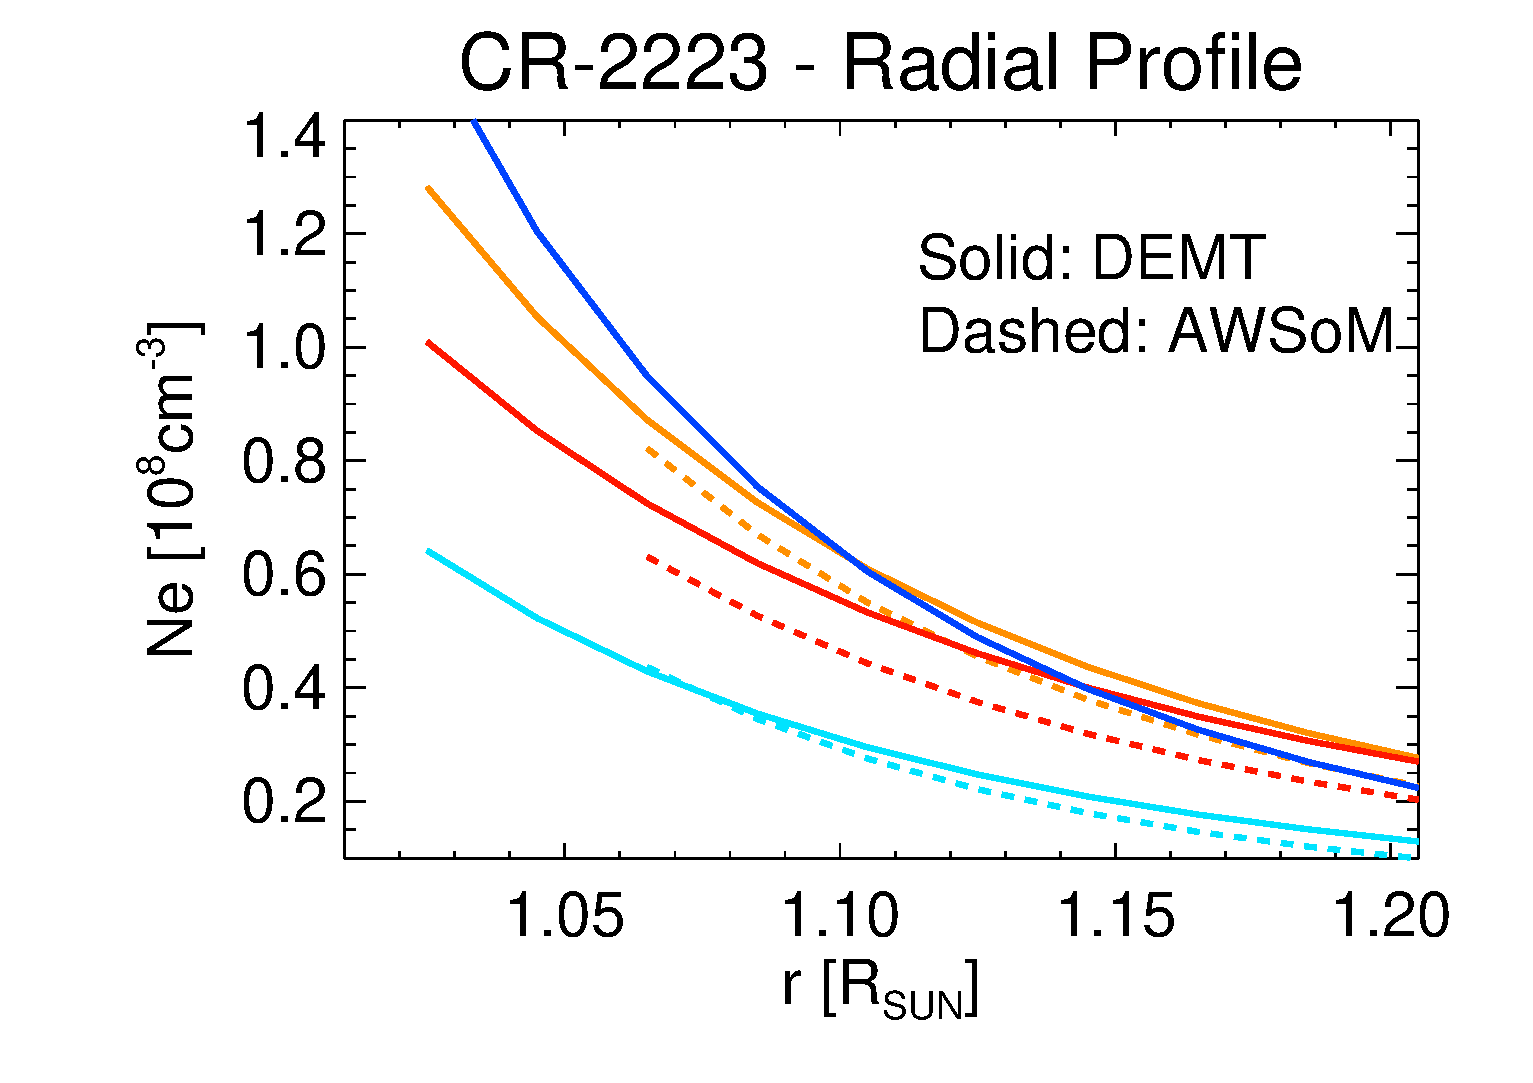
\includegraphics[width=0.99\textwidth,clip=]{figuras/perfil_paper_necr2223_bajo.eps}
\column{0.5\textwidth}
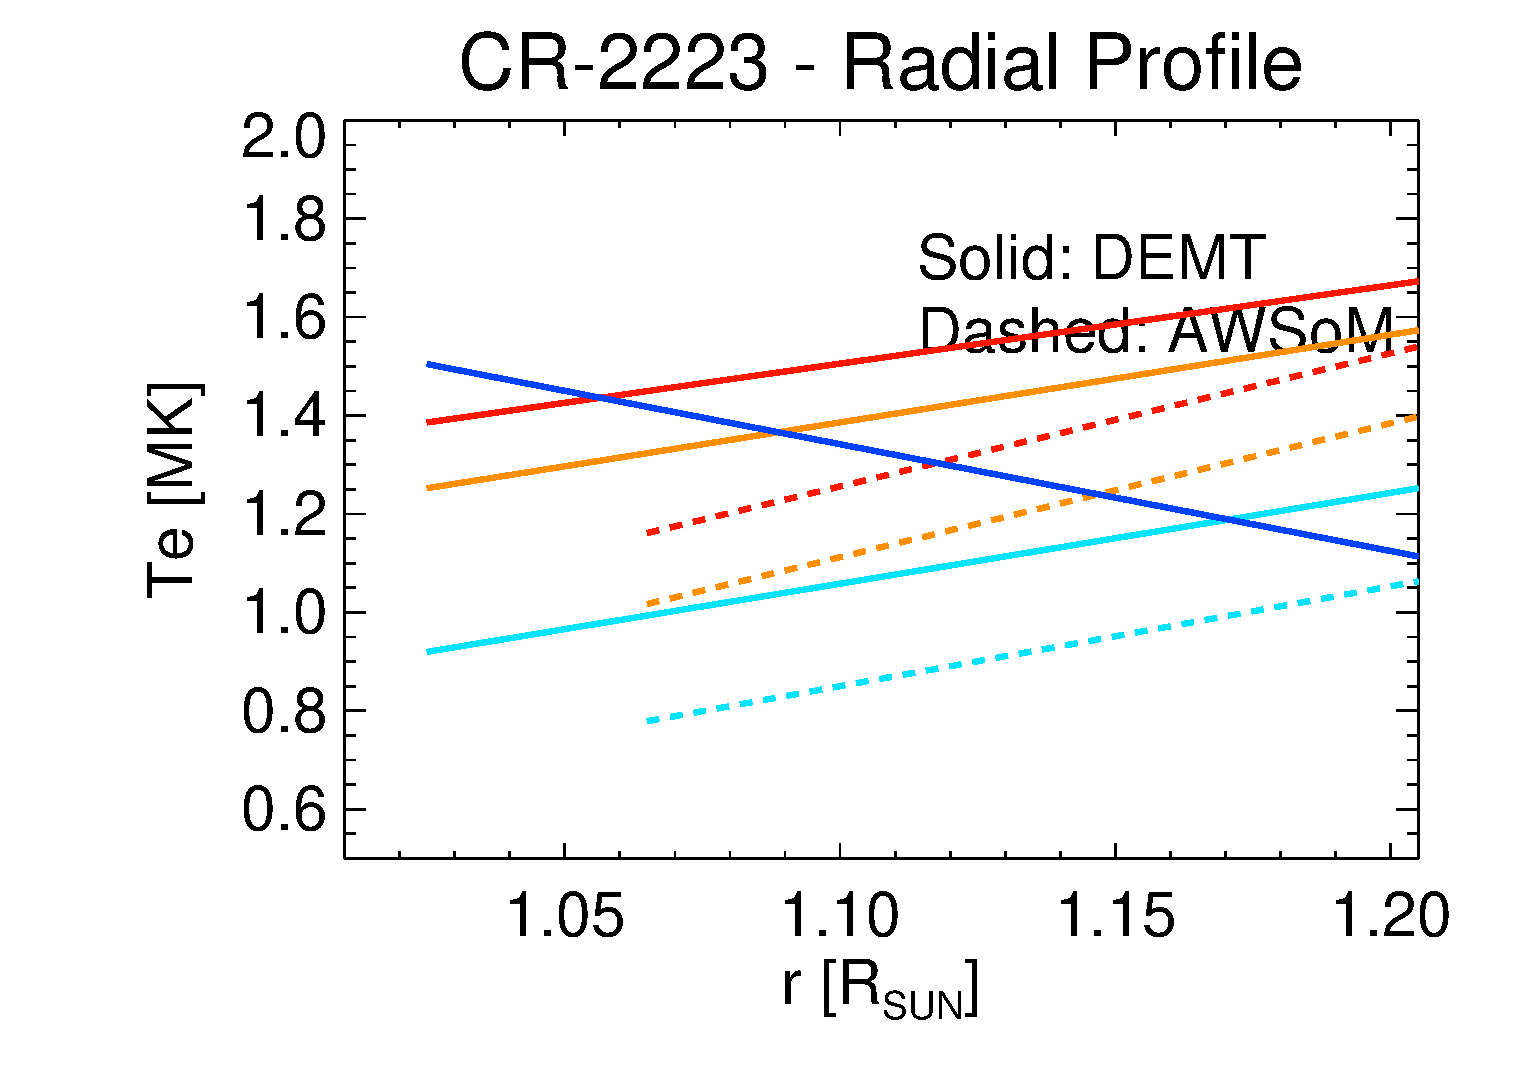
\includegraphics[width=0.99\textwidth,clip=]{figuras/perfil_paper_tecr2223_bajo.eps}
\end{columns}
\vskip 0.2cm
\bu Streamer (T0 $\rightarrow$ TII): $N_{CB}$ decrease; $\lambda_N$ y $\left<T_m\right>$ increases. \\
\vskip 0.2cm
\bu CHs (T III): $N_{CB}$, $\lambda_N$ y $\left<T_m\right>$ decrease.\\
%\bu $\Delta\Ne(r) \approx \pm 5\%$.
%\bu $\Delta\Te(r) \approx -15\%$.\\
}

%---------------------------------------


\frame{
\begin{columns}
\column{0.8\textwidth}
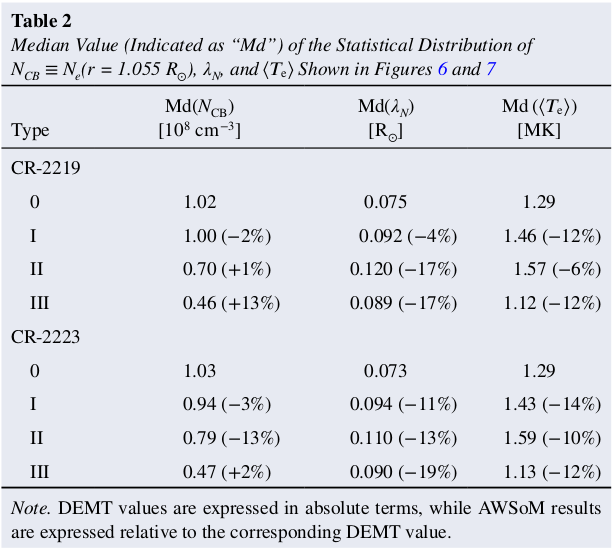
\includegraphics[width=0.99\textwidth,clip=]{figuras/tabla2_paper_2022.png}
\column{0.2\textwidth}
\vskip 0.5cm
\bu $E_N \approx 10\%$.\\
\bu $E_T \approx 5\%$.\\
Nuevo et al. (2015)\\
Lloveras et al. (2017)\\
\vskip 0.5cm
$\Delta\Ne \approx \pm 5\%$.\\
$\Delta\Te \approx -15\%$.\\

\end{columns}

}
%---------------------- DEMT vs AWSom
%\frame{ 
%\titulo{DEMT vs. AWSoM}
%\scriptsize
% Objetivo: Validar la capacidad del modelo en reproducir las reconstrucciones.
%\bu Motivación: Es AWSoM capaz para reproducir las reconstrucciones tomográficas?
%\vskip -0.2cm
%\begin{center}
%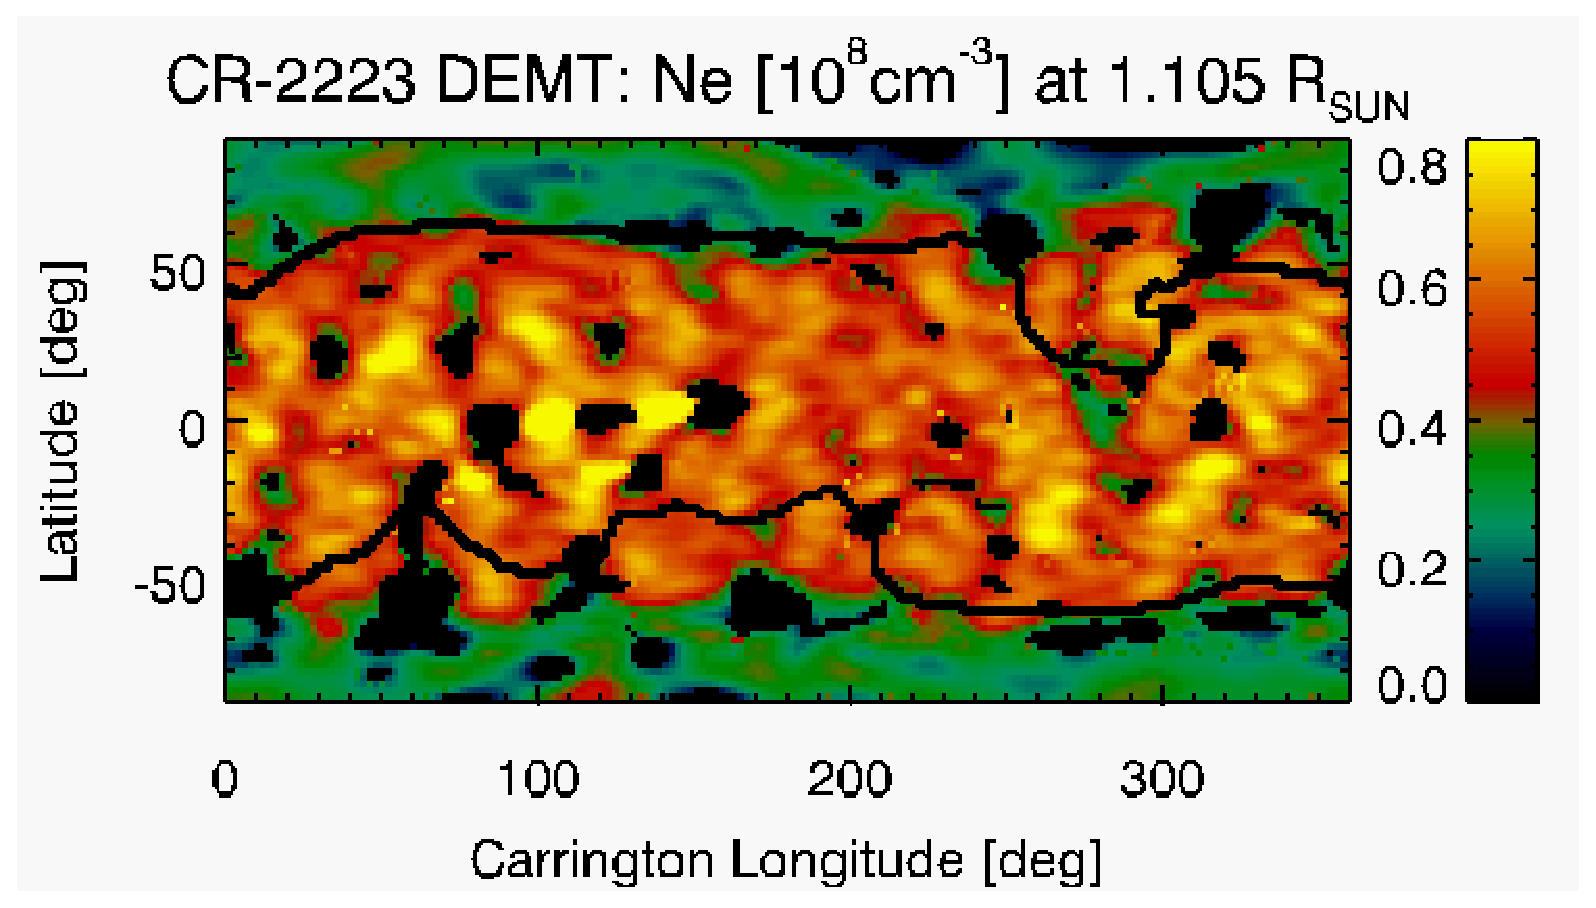
\includegraphics[width=0.495\textwidth,clip=]{figuras/map_Ne_CR2223_DEMT-AIA_H1_L733_r3d_multistart_1105_Rsun2223.eps}
%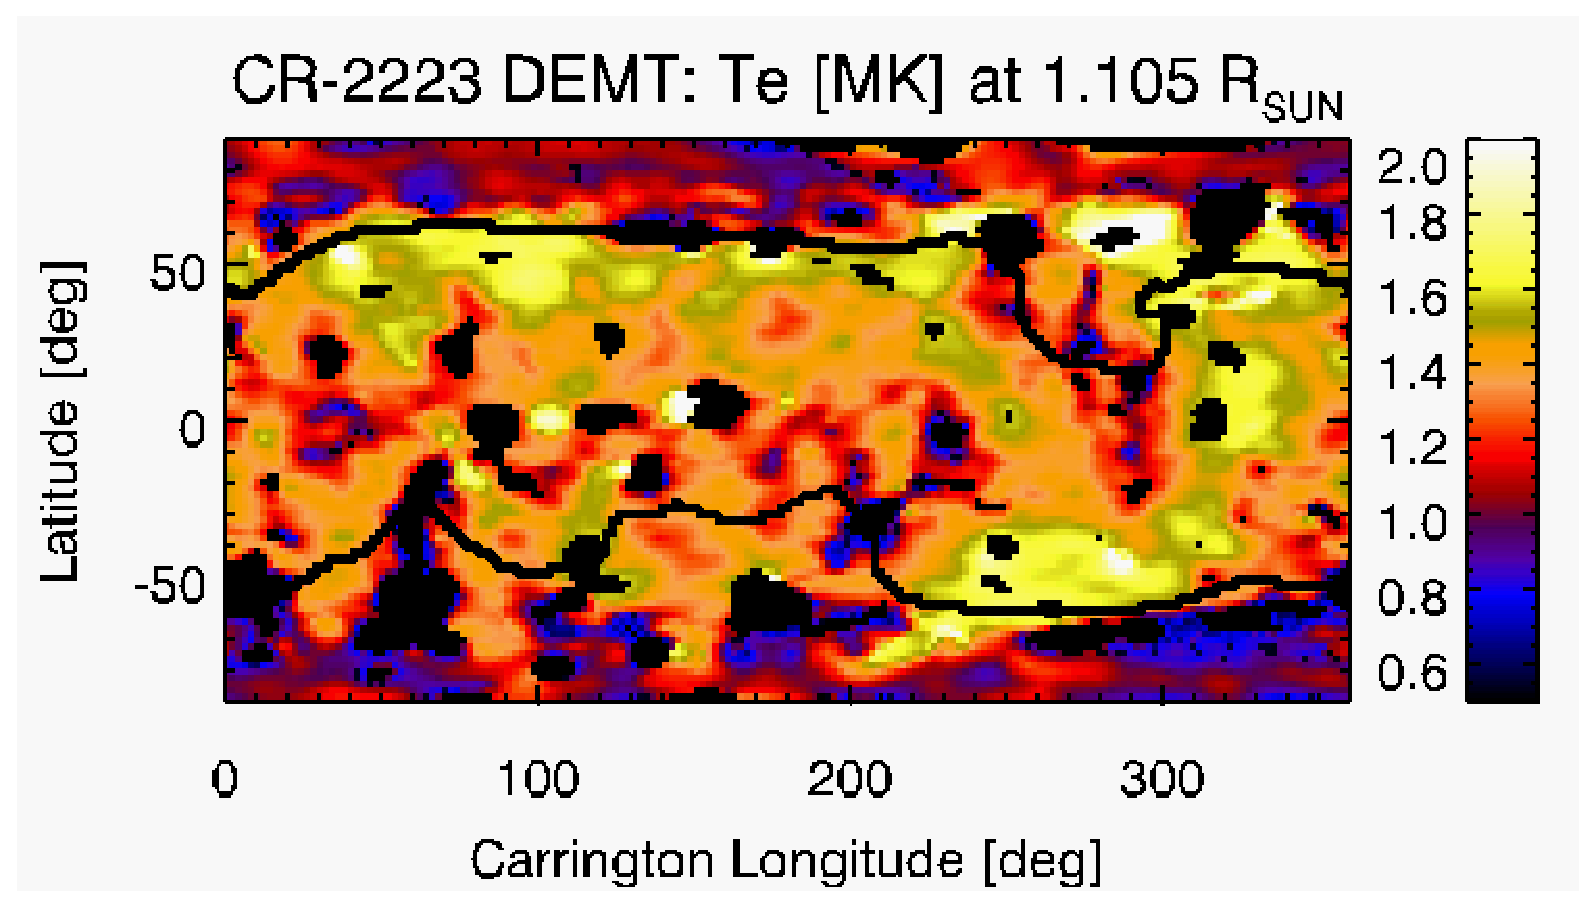
\includegraphics[width=0.495\textwidth,clip=]{figuras/map_Tm_CR2223_DEMT-AIA_H1_L733_r3d_multistart_1105_Rsun2223_2.eps}\\
%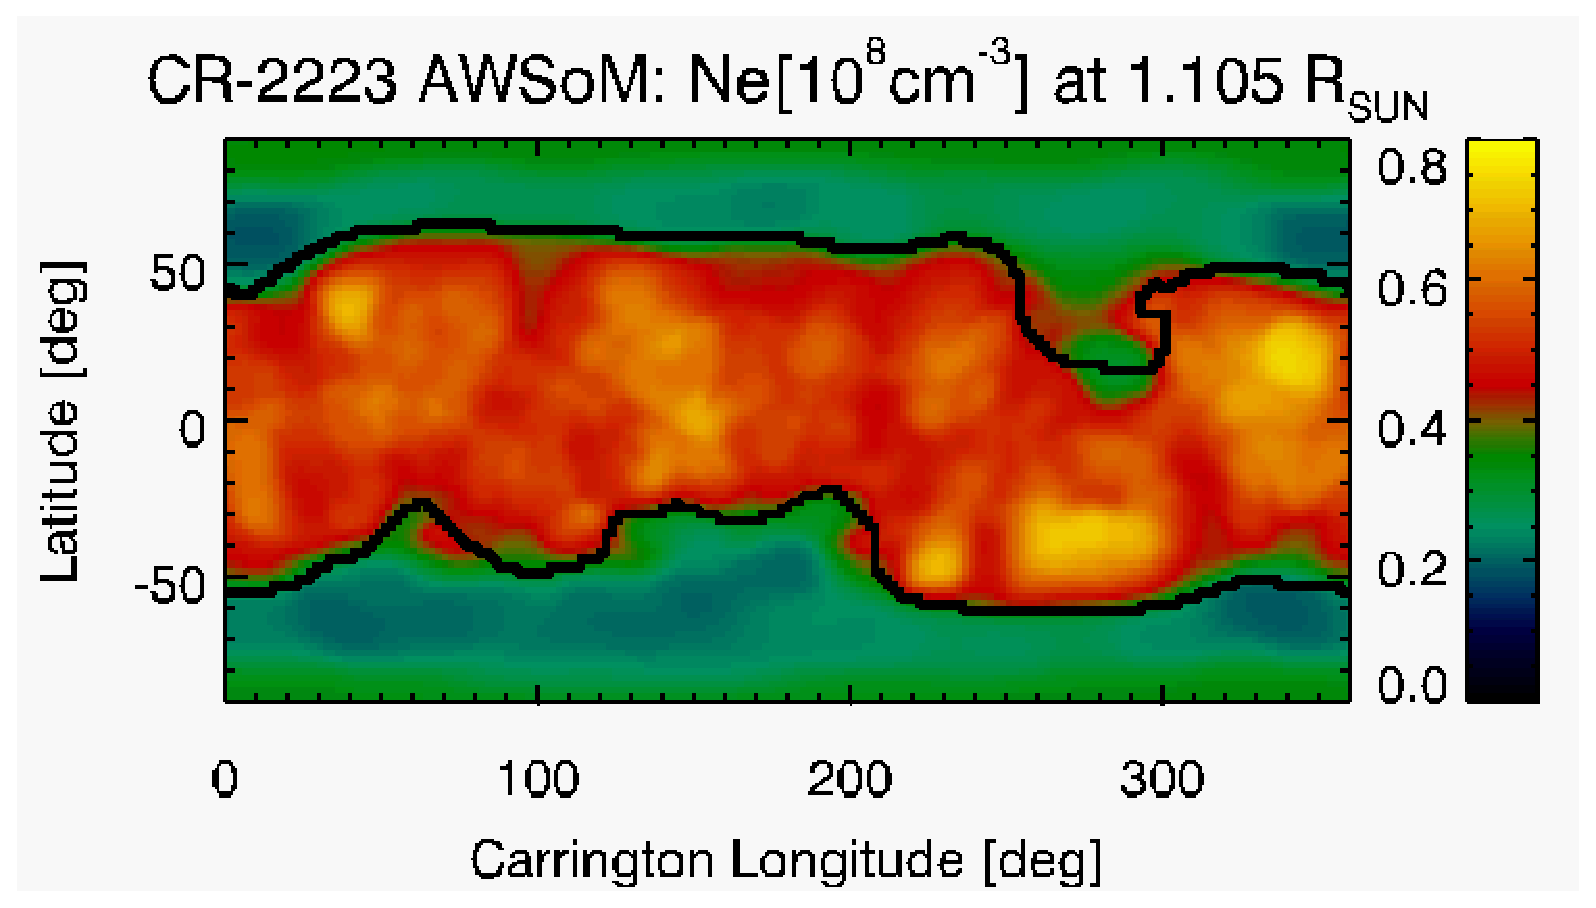
\includegraphics[width=0.495\textwidth,clip=]{figuras/map_Ne_awsom_2223_ener_new_1105_Rsun2223.eps}
%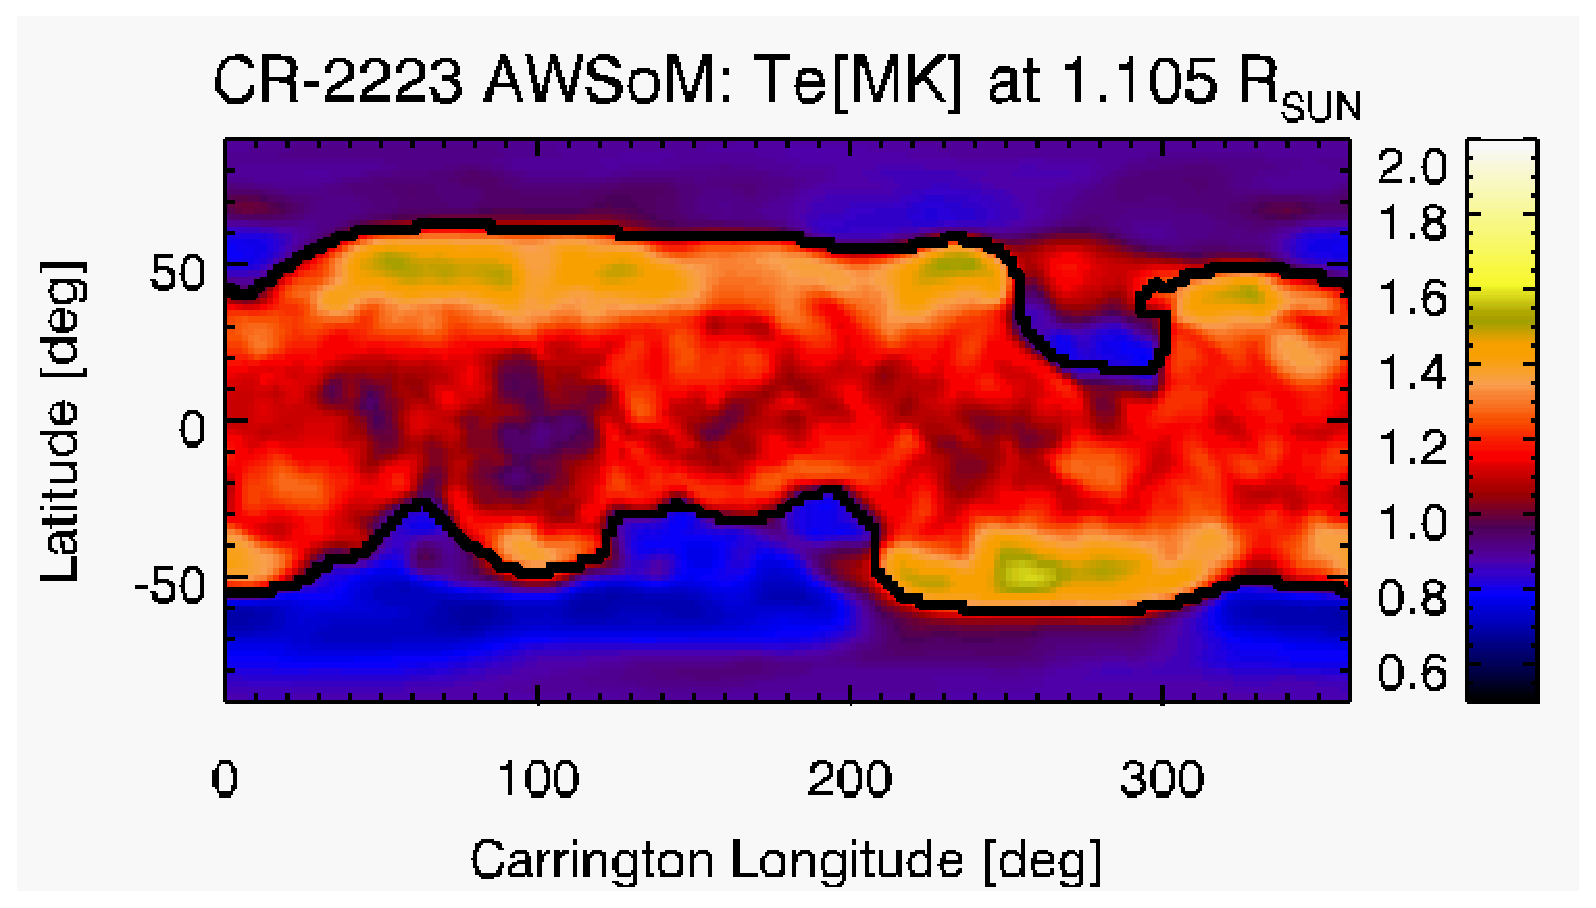
\includegraphics[width=0.495\textwidth,clip=]{figuras/map_Te_awsom_2223_ener_new_1105_Rsun2223_2.eps}\\
%\end{center}
%\begin{itemize}
%\item[\bu] En general hay buen acuerdo en magnitud y morfología de estructuras.\\
%\item[\bu] Diferencia en HS.
%\end{itemize}
%}


%-------------------------------

\frame{
\titulo{WL-SRT Validation of {\sc awsom}: Larger Heights}
\footnotesize
\begin{center}
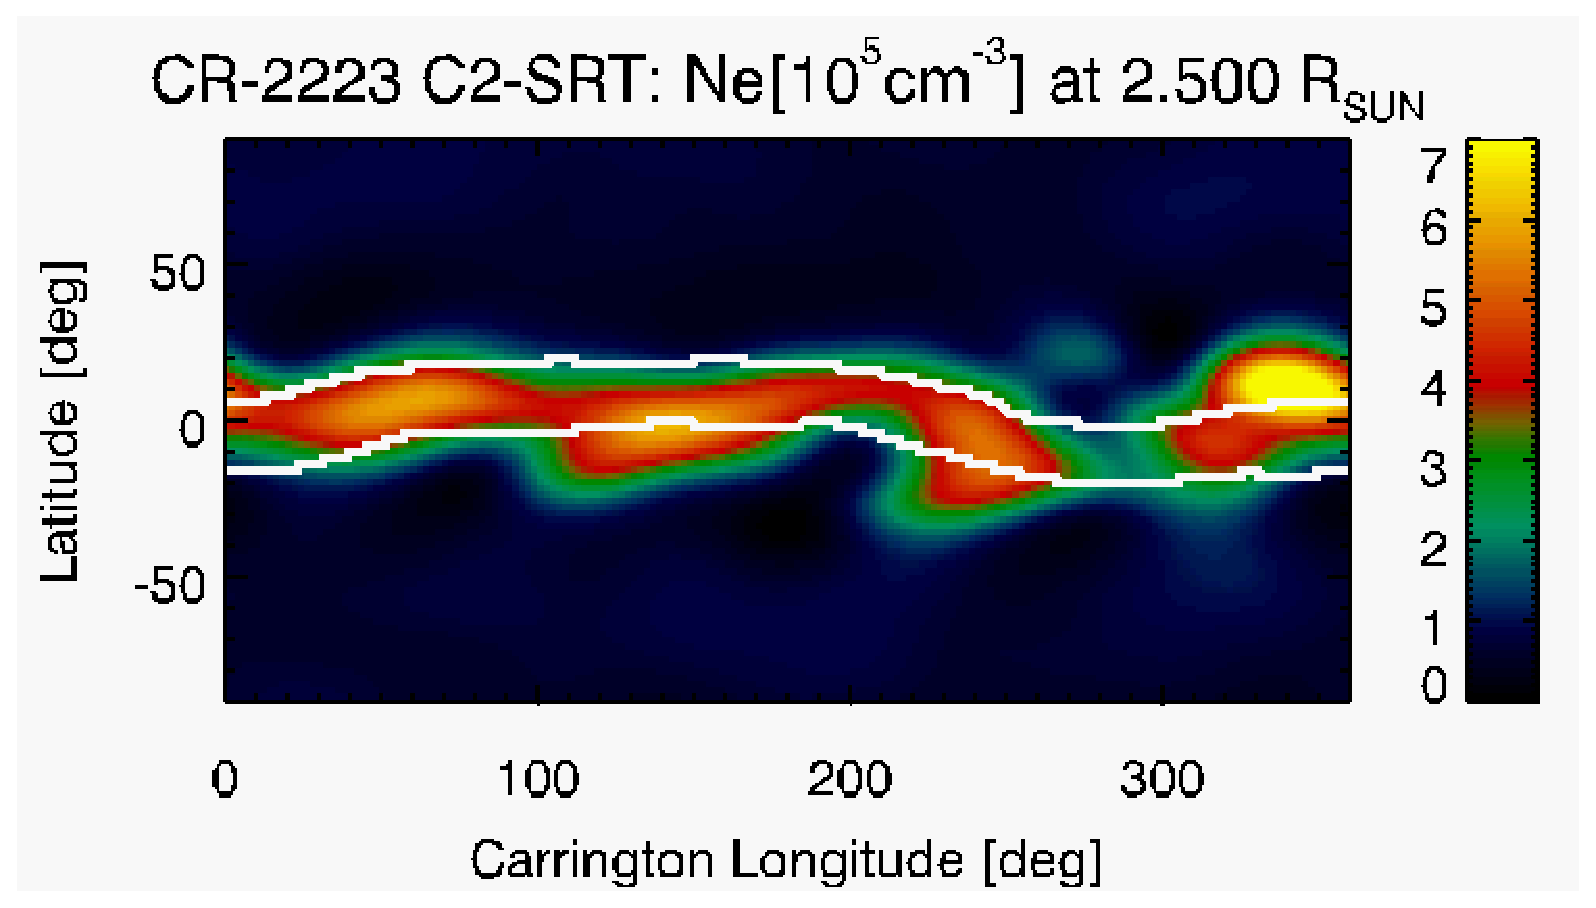
\includegraphics[width=0.45\textwidth,clip=]{figuras/map_LASCOC2pB_CR2223_24hr-Cadence_Rmin225_Rmax825_IRmin25_IRmax60_60x60x120_BF2_r3D_l25e-5_vfinal_interpolado_2500_Rsun2223.eps}
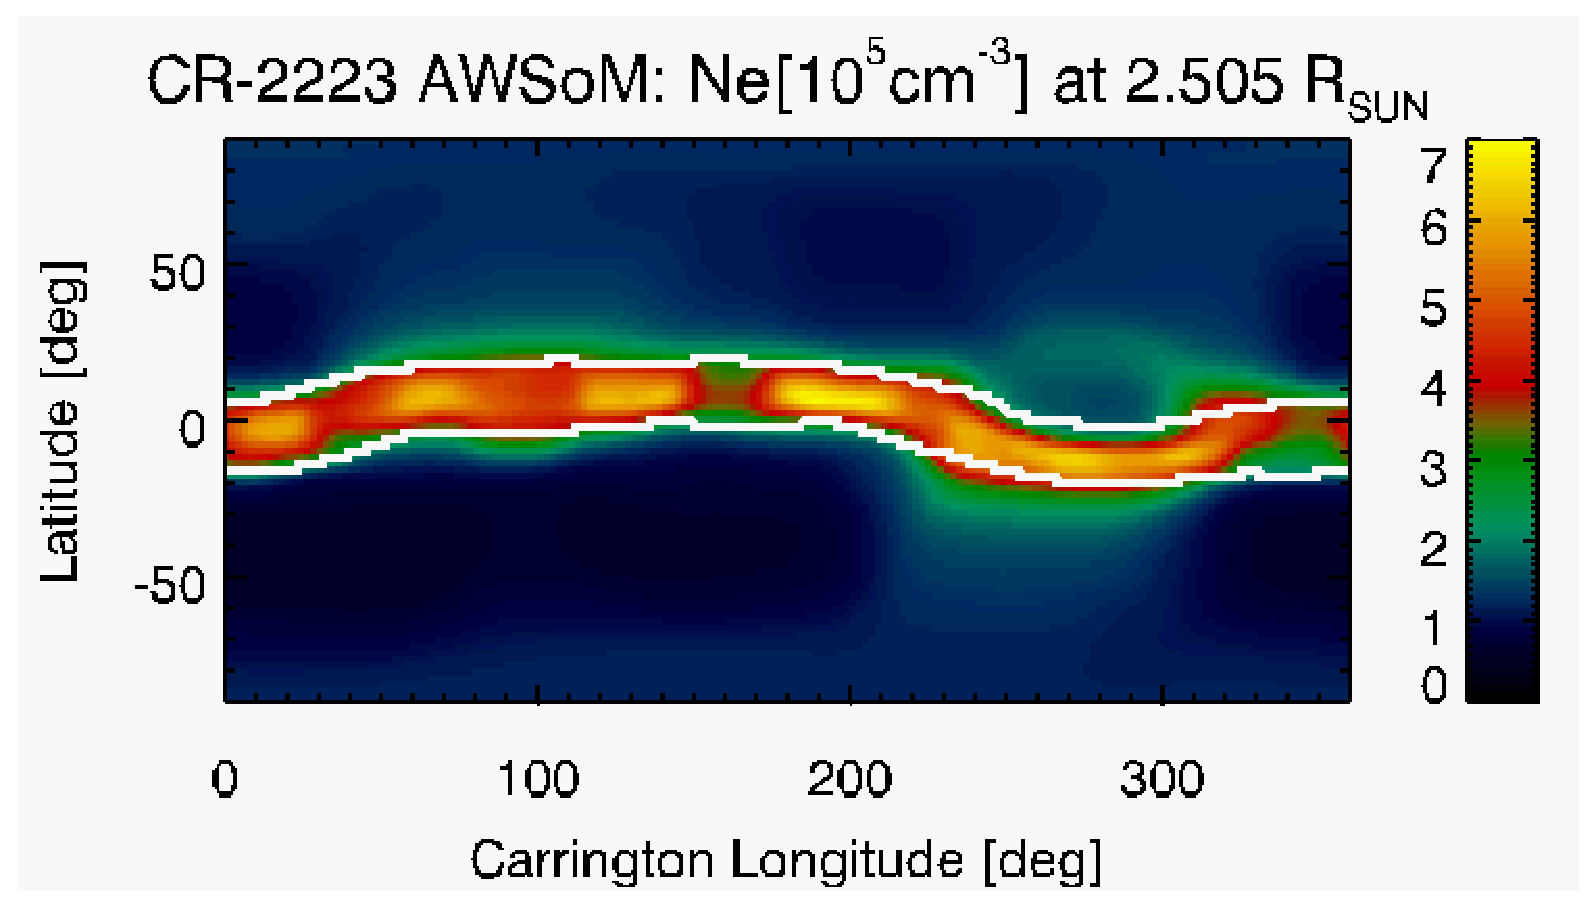
\includegraphics[width=0.45\textwidth,clip=]{figuras/map_Ne_awsom_2223_ener_new_2505_Rsun2219.eps}
%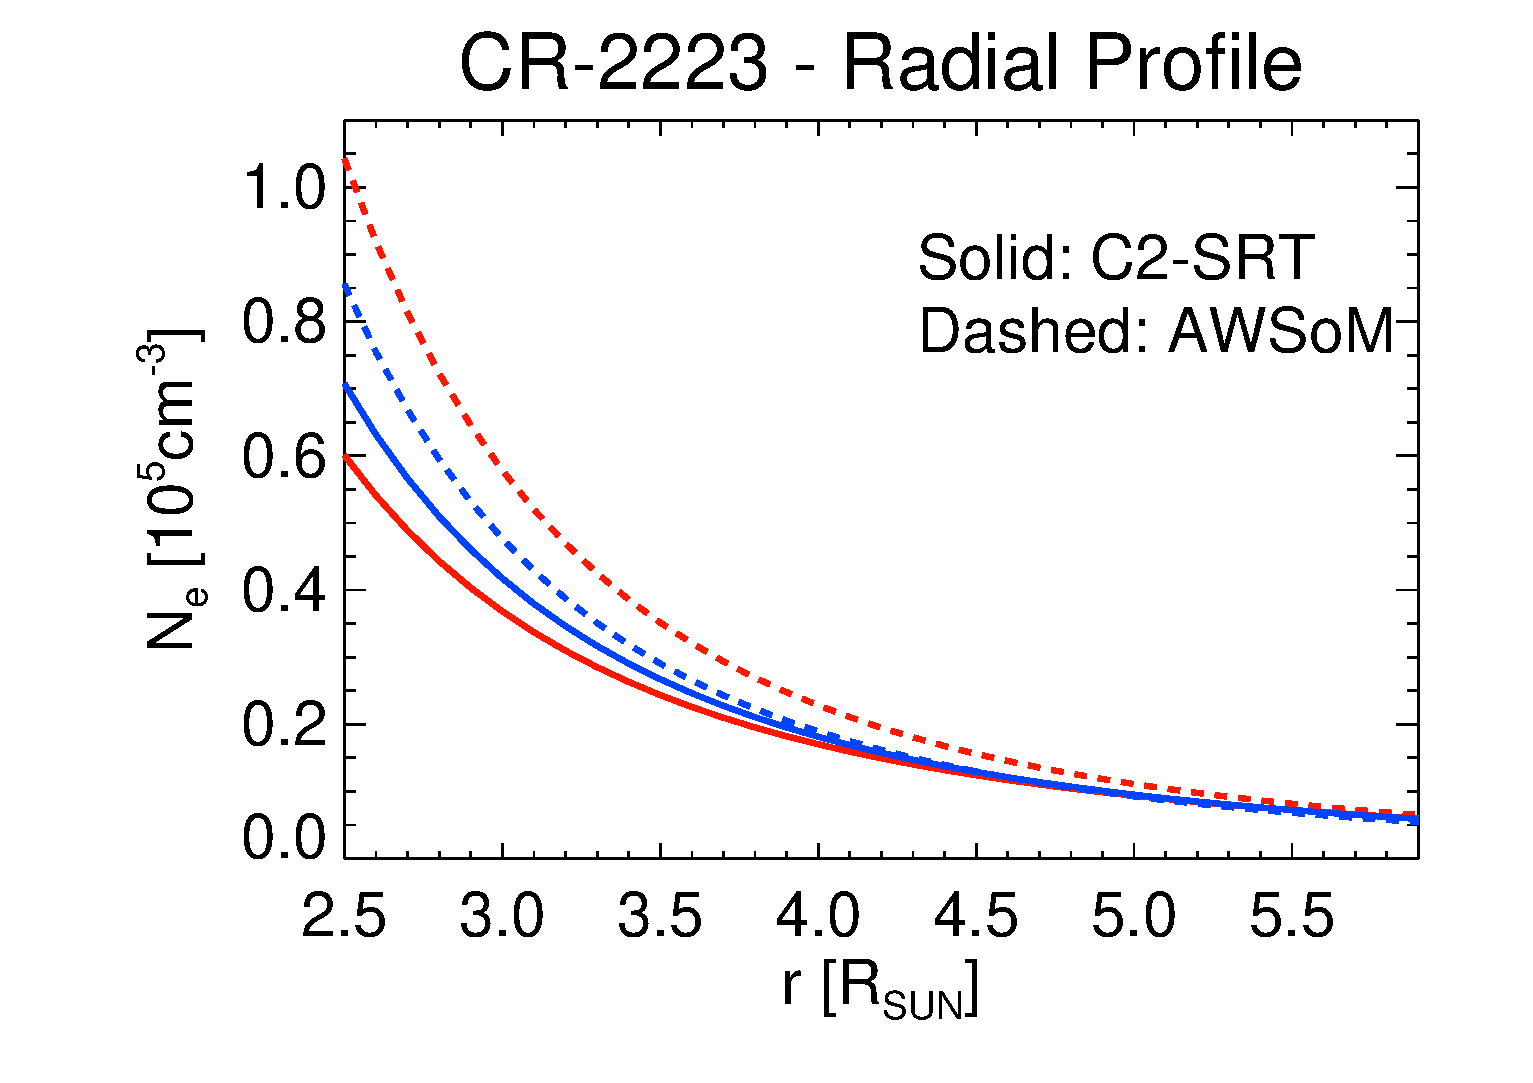
\includegraphics[width=0.28\textwidth,clip=]{figuras/perfil_paper_necr2223_alto_simplepot.eps}
\\
%$\Delta\Ne$ up to $+75\%$ at these larger heights $\rightarrow$ model's acceleration rates are too low.\\ 
%Current efforts include improvement in the energy cascading process of model.
\bu Good overall consistency in shape and size of Streamer and CHs.
\end{center}
\vskip .5cm
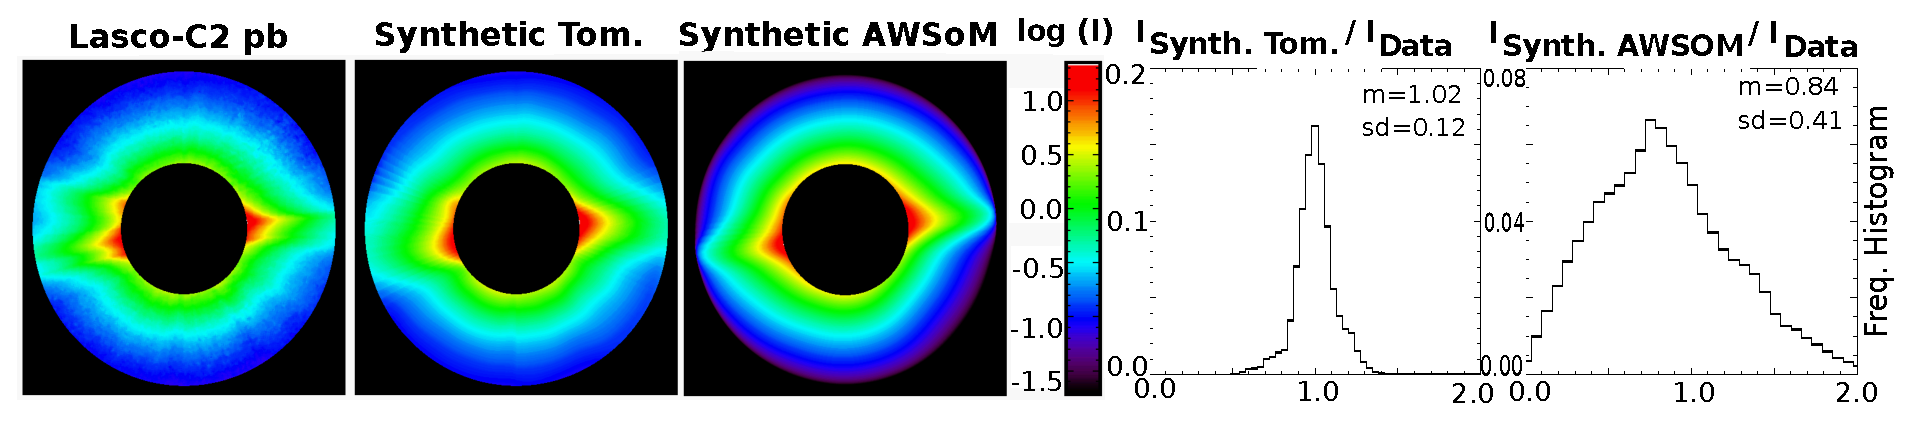
\includegraphics[width=\textwidth,clip=]{figuras/Figura_7_paper_imag_sintetica_2.eps}
%\vskip 0.75cm
$I_{Synt} \sim \int_{LDV} \mathrm{d}l \, N_e $\
}
%----------------------------------
\frame{
\titulo{Ne fit along B-lines}
\footnotesize
\bu Simple power law

\begin{center}
$N_e^{\rm (C2-SRT)}(r) = N_0\,\left(\,r/2.5\,\mrsun\right)^{-p} \rightarrow  \langle \l \rangle \equiv  \left\langle \left|  \frac{1}{{N_e(r)}} \, \frac{{{\rm d}N_e}}{{\rm d}r}(r) \right|^{-1} \right\rangle {= \frac{\langle r\rangle}{p} = \frac{4.25\,\mrsun}{p}} $ 
%\end{equation}
\end{center}
\bu Errors: \azul{$\Delta N_m \approx 20\%$} y \azul{$\Delta \left< \lambda_n \right> \approx 15\%$}

%\titulo{C2-SRT vs AWSoM: Comparación estadística}

\begin{center}
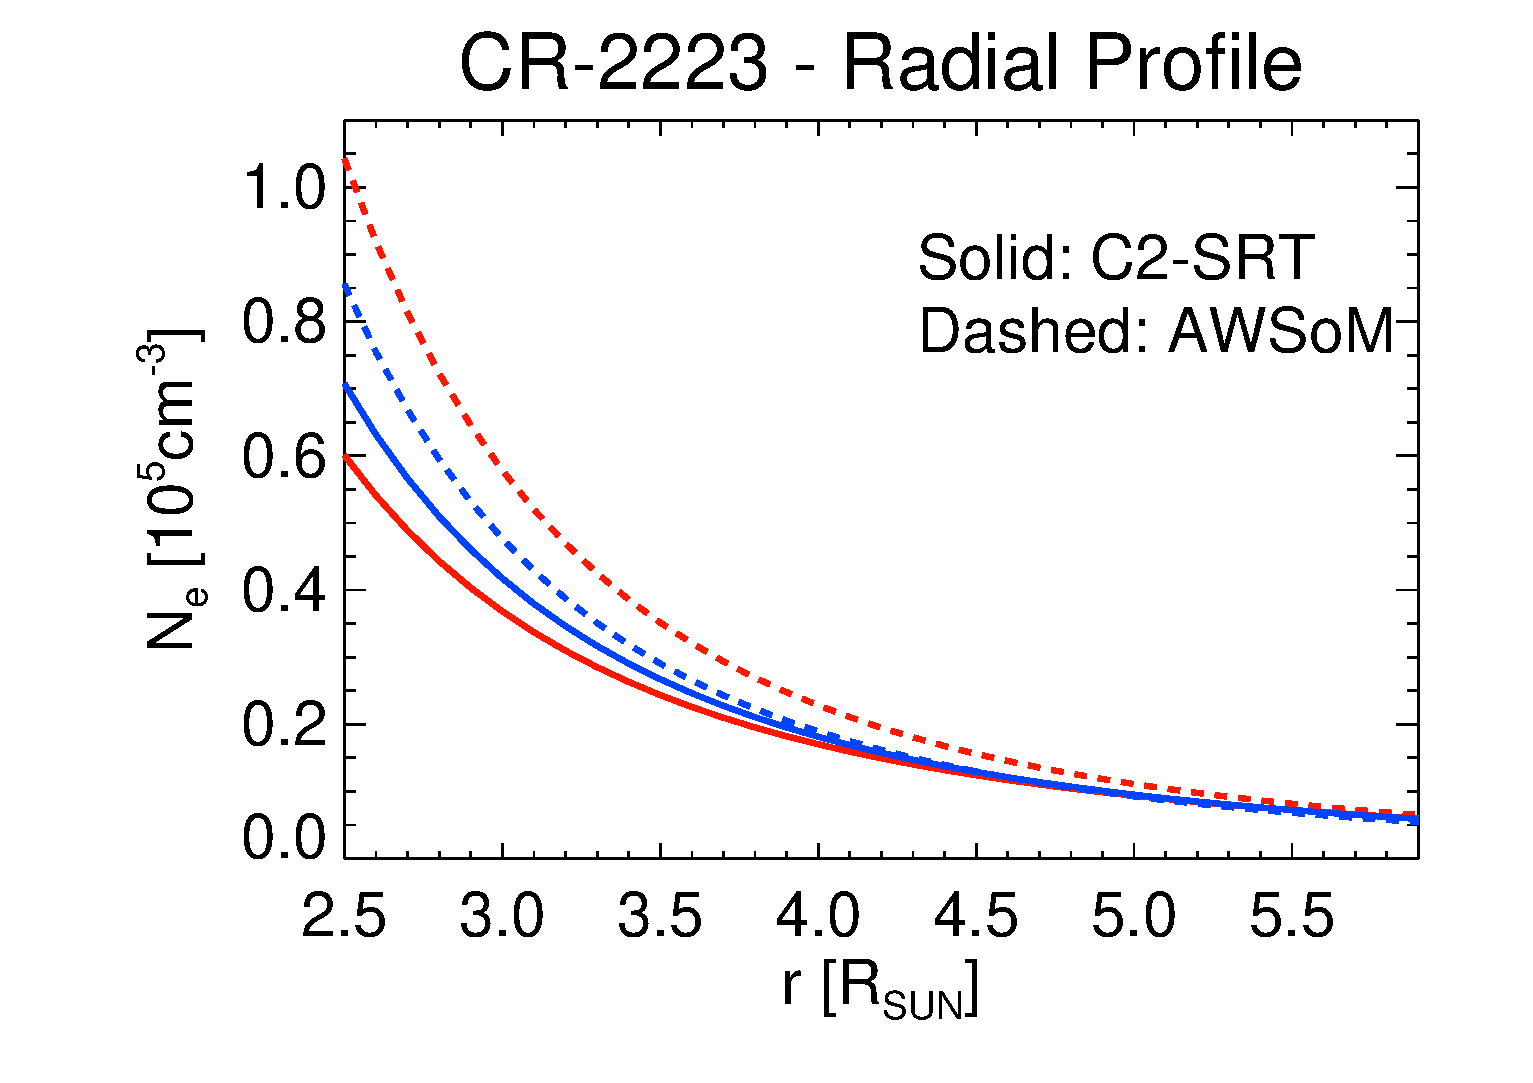
\includegraphics[width=0.5\textwidth,clip=]{figuras/perfil_paper_necr2223_alto_simplepot.eps}
\end{center}
%\end{columns}

\bu Ne$(r=2.5\,\mrsun) \approx 0.6-0.7\times 10^5\,{\rm cm}^{-3}$\\

\bu $\lambda_N\approx 1.4-1.6 \,\mrsun \rightarrow \left<p\right> \approx 2.8-3.3$ (consistent with other studies)\\

\bu AWSoM overestimate basal density up to 75\%  $\rightarrow$ model's SW acceleration rates are too low\\
%\, \, \, \, \, \, \, $\rightarrow$ solar wind acceleration is gradual and spread out

%$\Delta\Ne$ up to $+75\%$ at these larger heights $\rightarrow$ model's acceleration rates are too low.\\ 
%Current efforts include improvement in the energy cascading process of model.
}


%-------------------------------
\frame{
\titulo{Ne and Te in the source region of the Solar Wind}
\footnotesize
\begin{center}
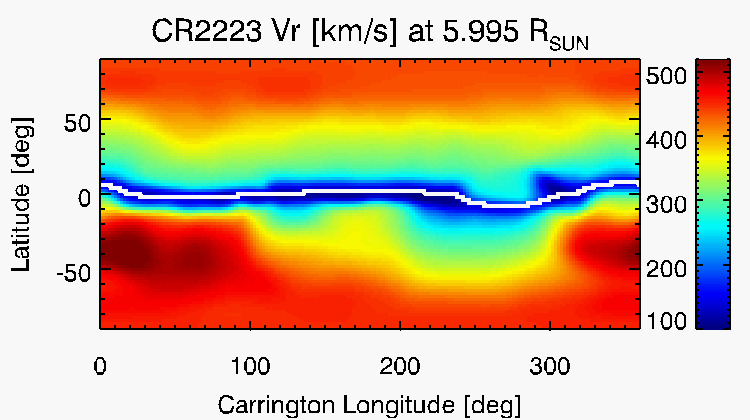
\includegraphics[width=0.45\textwidth,clip=]{figuras/map_Vr_awsom_2223_realization10_extended_new_5995_Rsunsom_.jpg}
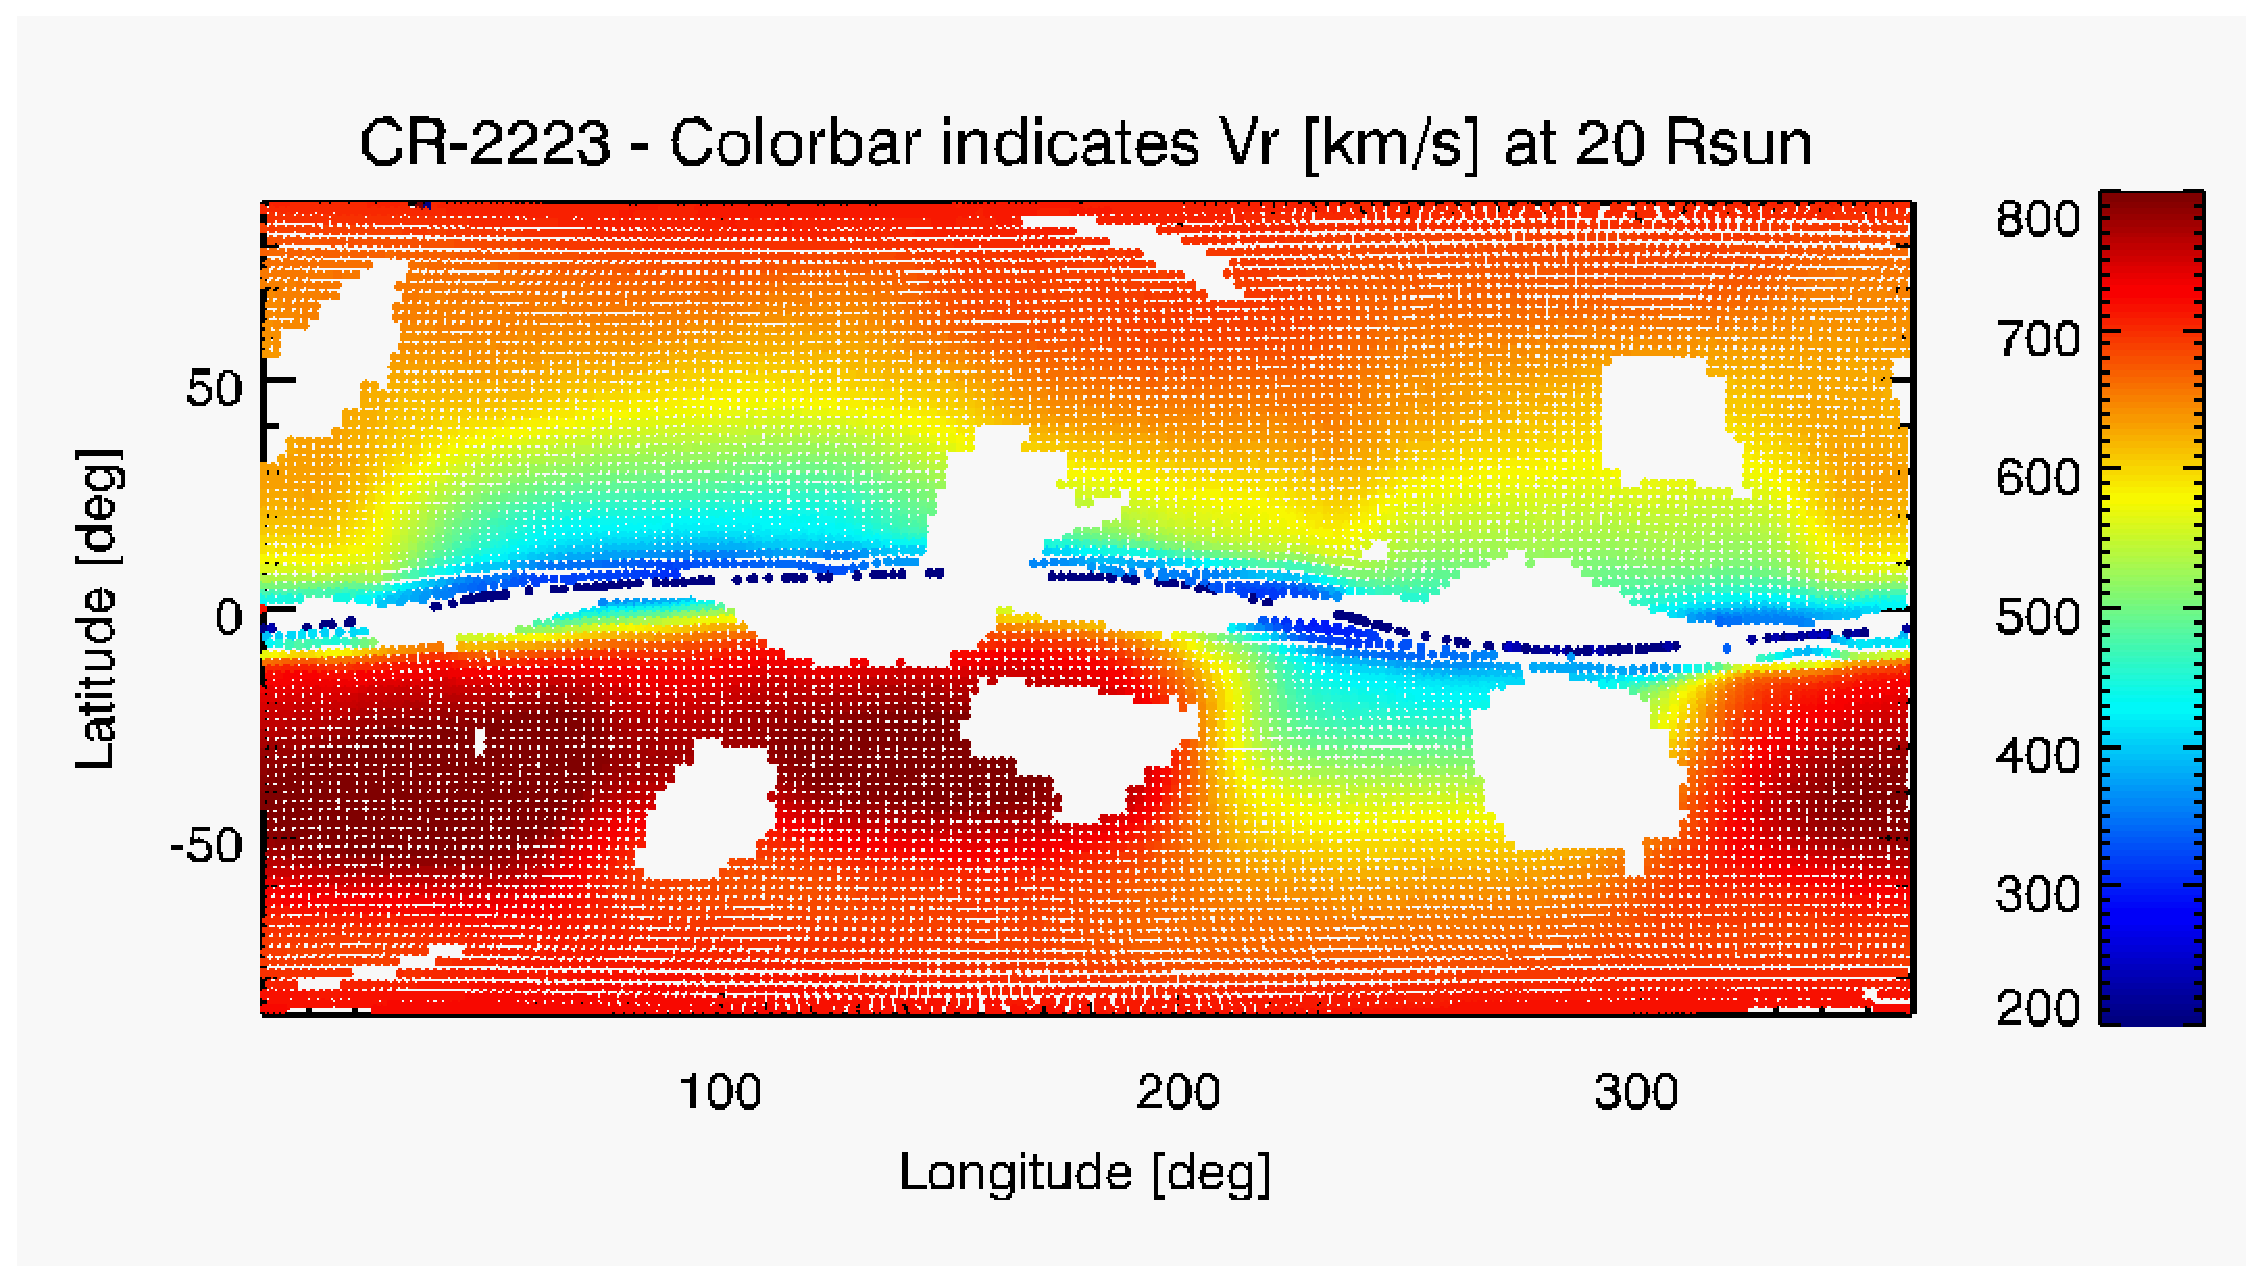
\includegraphics[width=0.45\textwidth,clip=]{figuras/scatter_plot_Vr_newtrace_20_CR-2223_filtro.eps}
\\
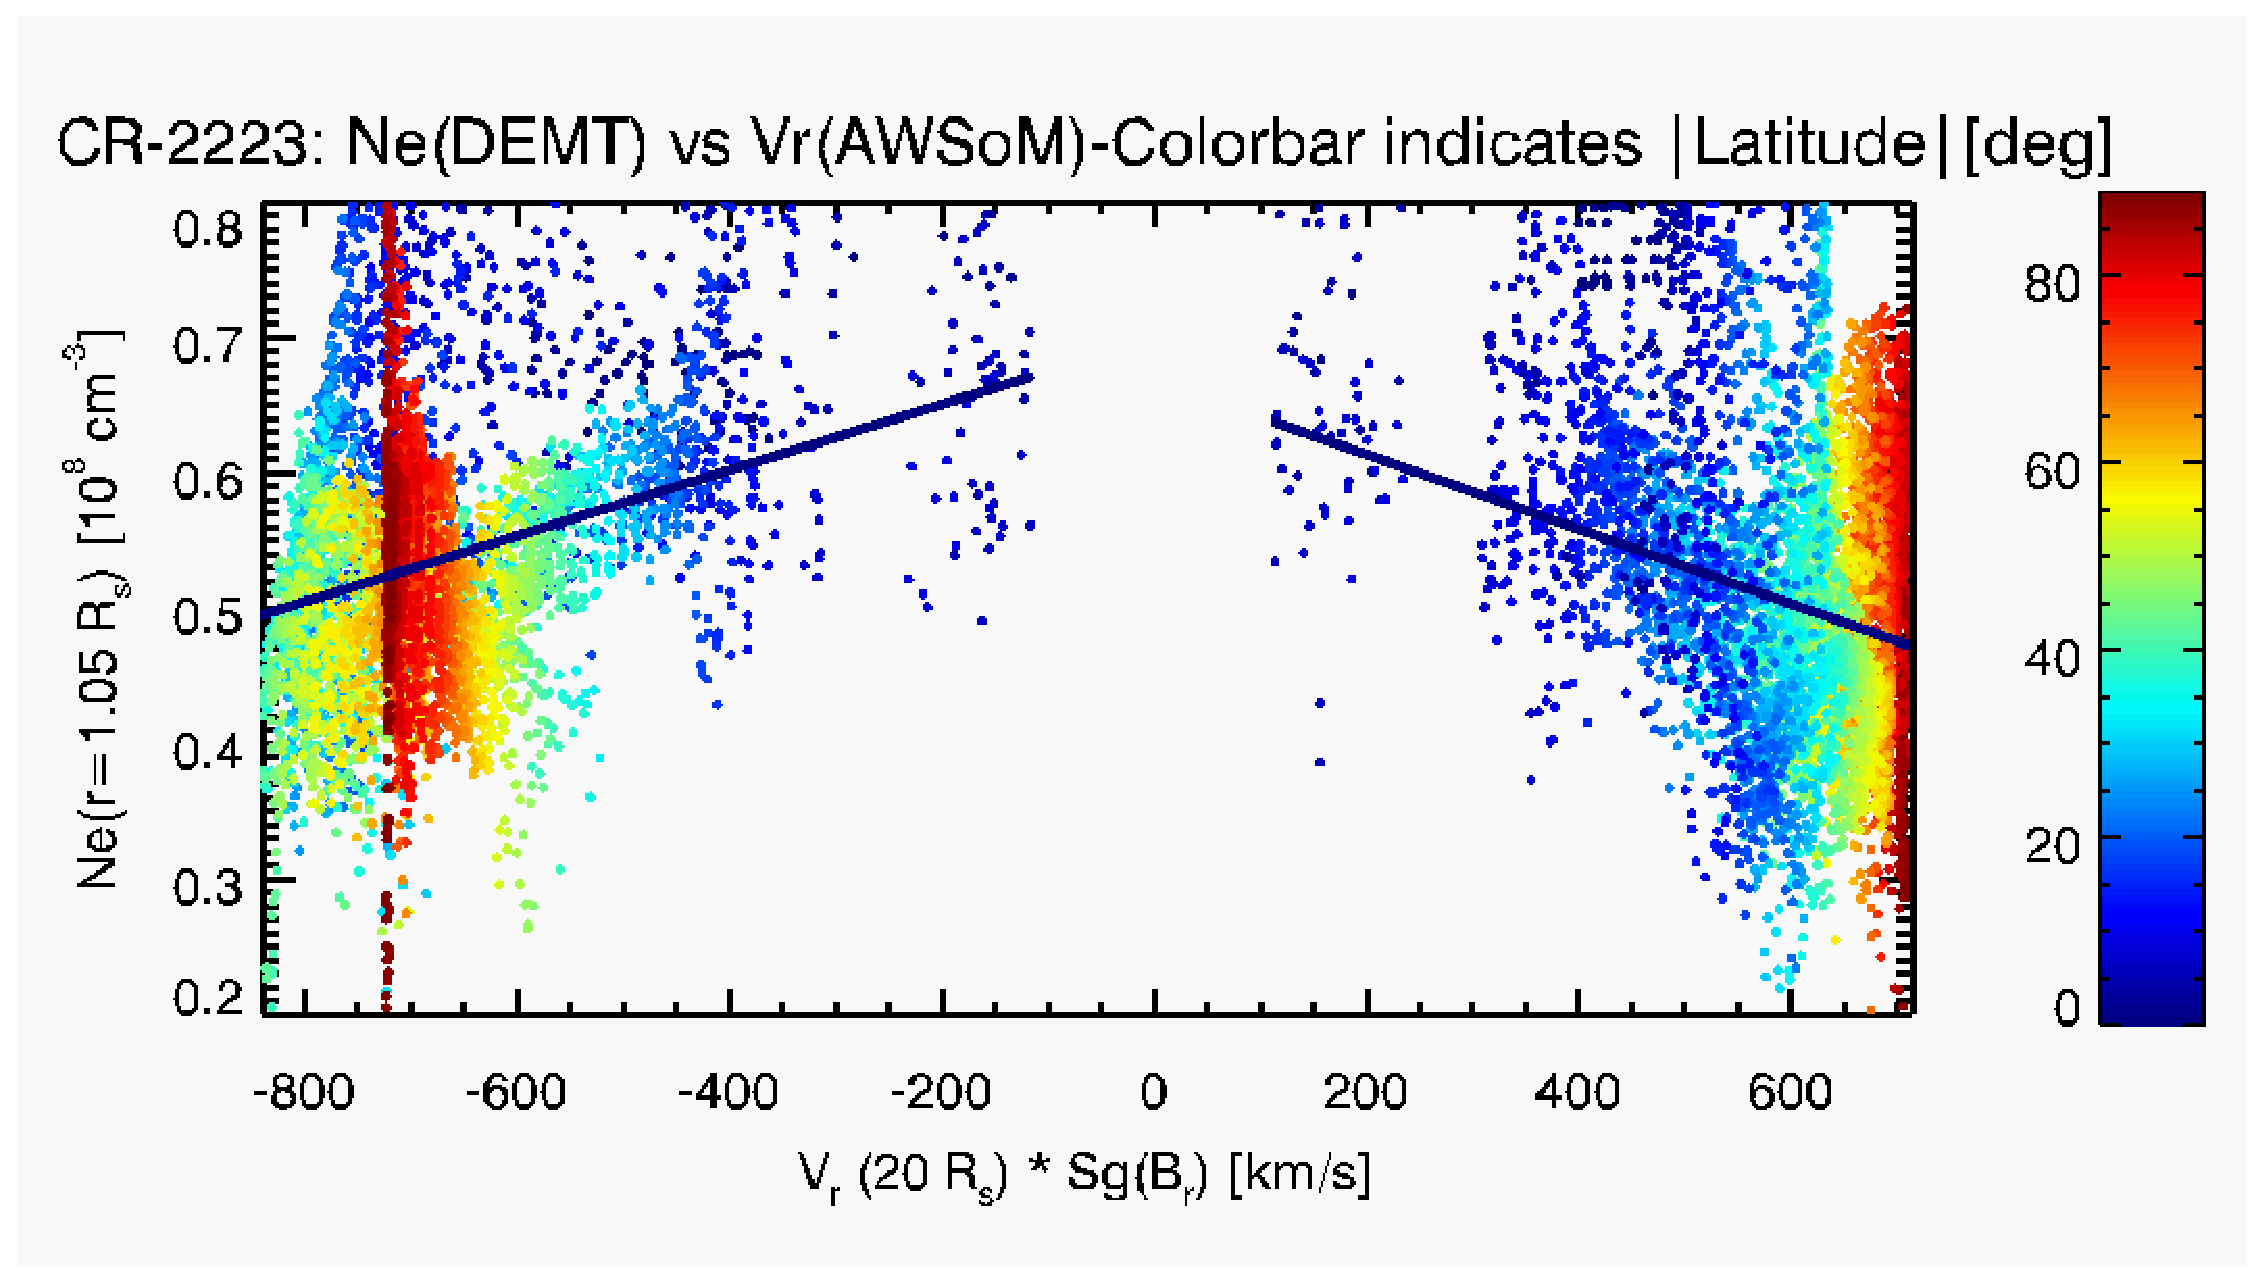
\includegraphics[width=0.45\textwidth,clip=]{figuras/scatter_plot_nedemtFIT_1055_vs_vrxsignoBr_20rs_CR-2223_trace_chip_.eps}
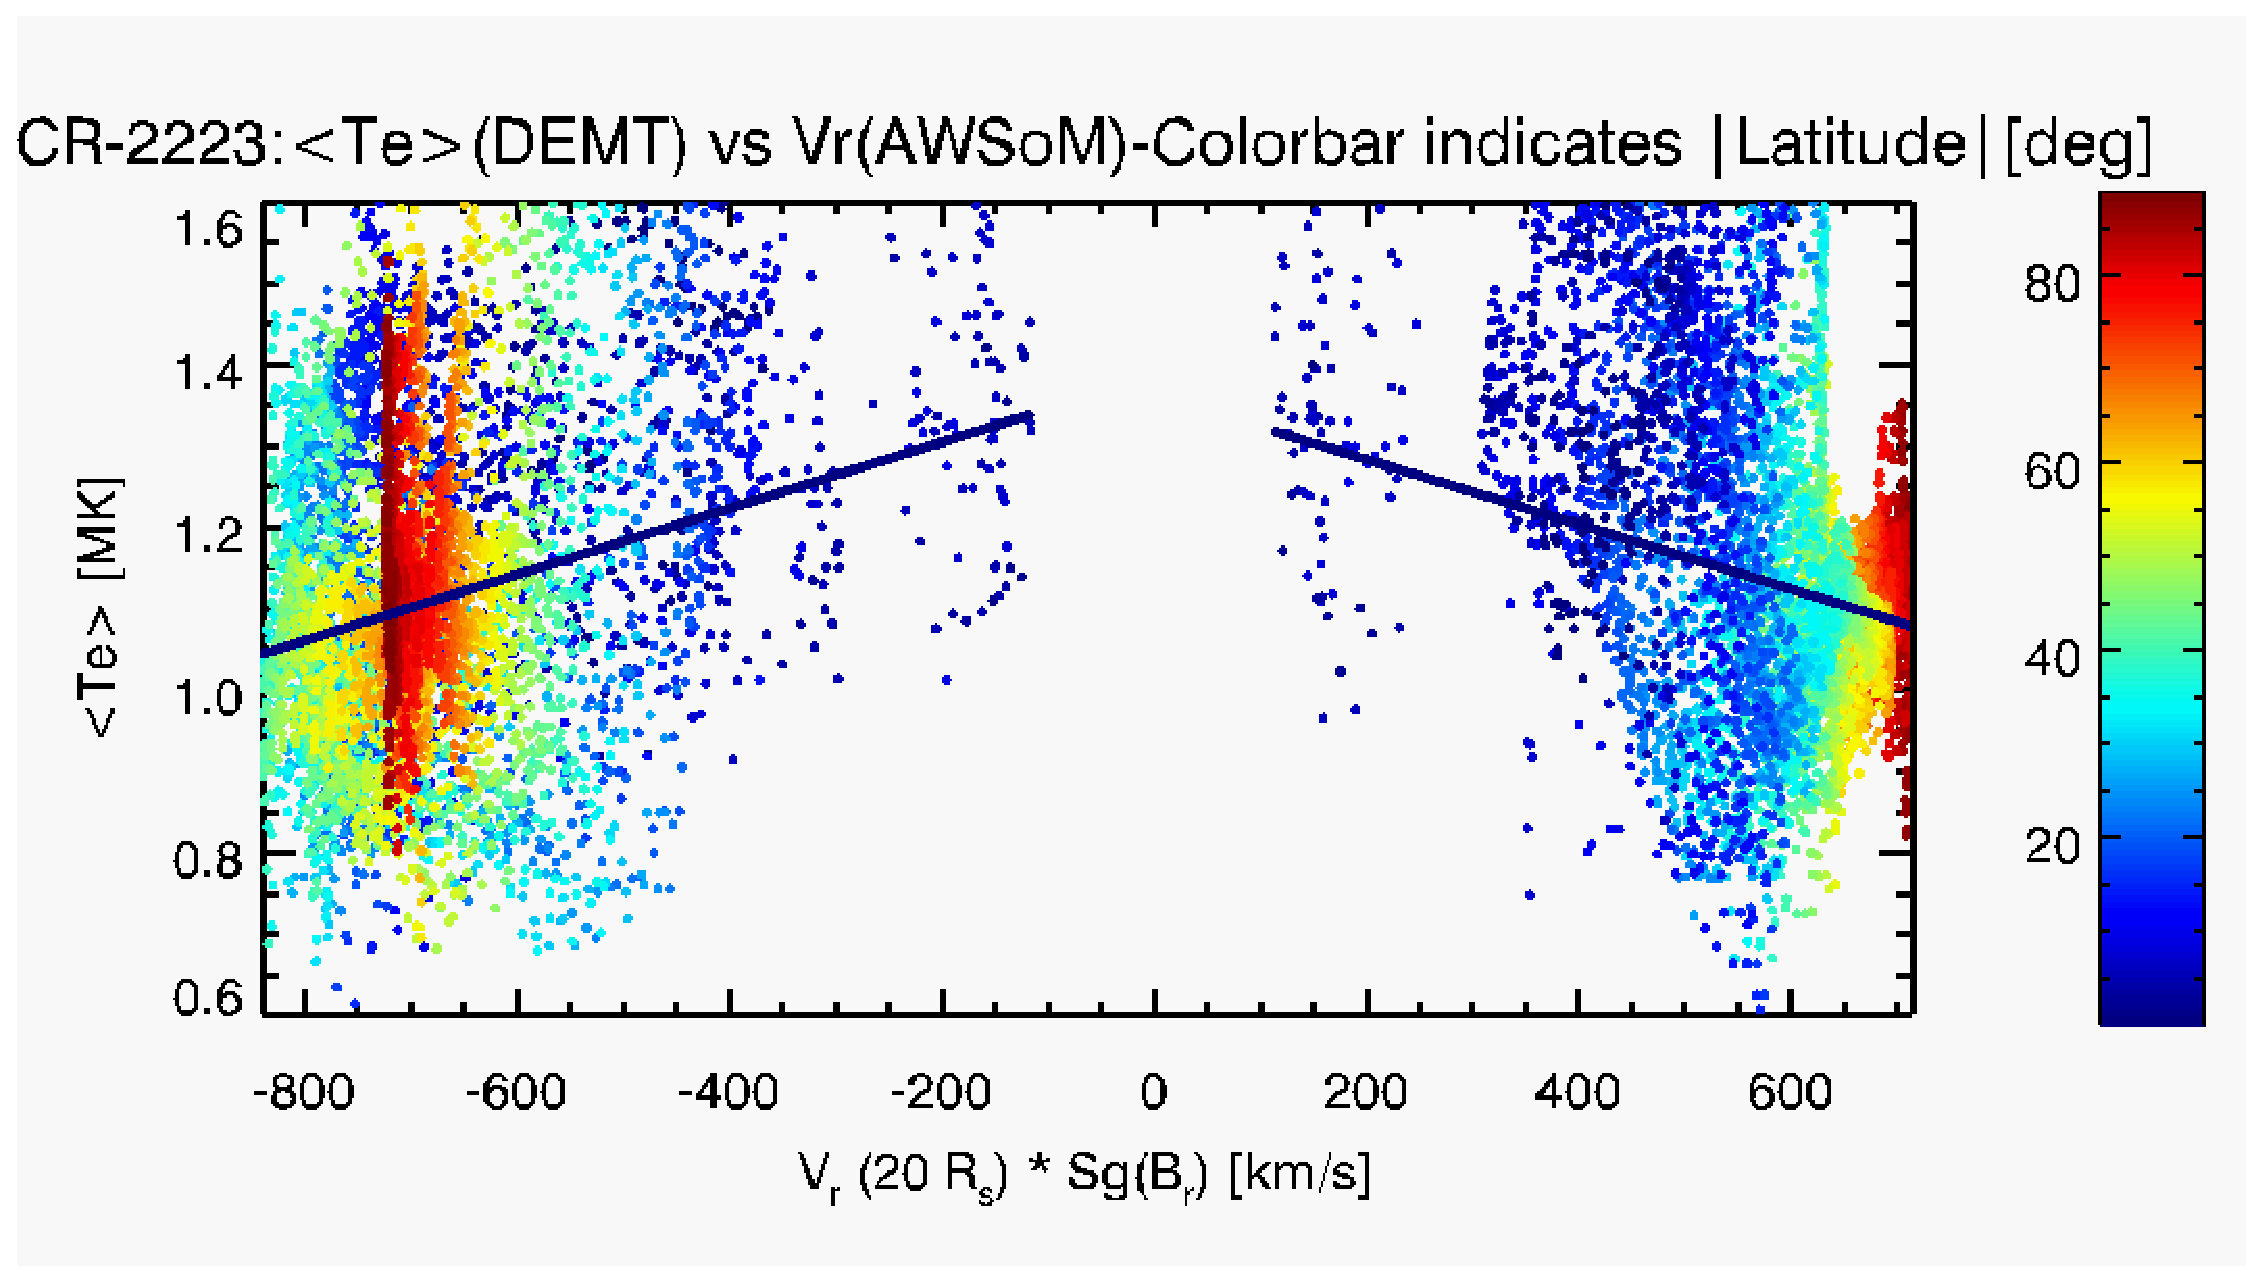
\includegraphics[width=0.45\textwidth,clip=]{figuras/scatter_plot_tmdemt_MEAN_vs_vrxsignoBr_20rs_CR-2223_Test_trace_chip_.eps}
\end{center}
\bu Model's terminal wind speed anticorrelates with DEMT $\Ne$ and $\Te$ at source region.
\vskip 0.1cm
\bu Consistent with stable highly ionized slow wind flowing around Streamers $\rightarrow$\\
\hskip 0.3cm
No reconection process required (Oran et al., 2015).
}

%------------------------
\frame{
\titulo{Conclusions}

\begin{itemize}
%DEMT\\
  \item[\bu] We characterize the thermodynamic structure of the corona. Trends are all in accordance with previous DEMT studies (Lloveras et al., 2017, 2020).
  \item[\bu] Compared to CRs 2081/2082 (during the SC 23/24 deep minimum epoch), the WHPI targets exhibit a 20\% lower coronal base density, and 20\% larger scale height and electron temperature.
%AWSom  
  \item[\bu] AWSoM in comparison with DEMT: good agreement in Ne, and Te is up to 20\% smaller (beyond uncertainty).
  \item[\bu] AWSoM in comparison with C2-SRT: Ne of the model is up to 75\% larger (beyond uncertainty). Likely due to the acceleration of SW being more gradual and extended than observed.
  %Solar Wind
  \item[\bu] The model's terminal wind speed along field lines is anti-correlated with reconstructed DEMT values of Ne and Te at the source region.
%  \vskip 0.3cm
%  \item Hallamos la presencia de arcos down en los tres mínimos.
%  \vskip 0.3cm
%  \item Por primera vez aplicamos simultáneamente la técnica tomogáfica utilizando imágenes EUV y LB. Esto constituye una valiosa herramienta de condicionamiento para la validación y el desarrollo de modelos MHD 3D que tengan como objetivo la predicción meteorológica espacial.
%  \vskip 0.3cm
%  \item Estudiamos la relación entre el campo de velocidad terminal del viento y la densidad y temperatura en su región fuente.

\end{itemize}
}
%---------------
\begin{comment}
\frame{ 
\titulo{Conclusiones DEMT}

%conclusion DEMT de comparacion de 3 mínimos. \\
\footnotesize


\btr Características generales:\\
\bu Los Streamers exhiben $N_{CB} \approx 1.0-1.2\times 10^8\,{\rm cm}^{-3}$, los CHs se caracterizan por una densidad del orden de la mitad. \\
\vskip 0.2cm
\bu $\lambda_N \approx 7-11\times 10^{-2}\,\mrsun$, con los valores menores correspondiendo a las latitudes más bajas del streamer y a los CHs. \\
\vskip 0.2cm
\bu Los streamers se caracterizan por $\left<T_m\right>\approx 1.2-1.6$~MK (con las temperaturas menores correspondiendo a las latitudes más bajas) mientras que los CHs exhiben $T_{m} \lesssim 1$~MK.\\
\vskip 0.2cm
\bu Hallamos la presencia de loops down en los 3 mínimos. Nuevo et al. (2013); Schiff and Cranmer (2016). Presenta condicionamiento al modelo de calentamiento coronal.\\
%Correlación entre número de líneas tipo 0 y mínimo de actividad.\\
%$\beta > 1$ favorece la conversión de ondas de Alfvén en modos compresibles.\\

\vskip 0.7cm
\btr Comparación de los últimos 3 mínimos:\\
\bu $\left<T_m^{SC \, 22/23}\right>  > \left<T_m^{SC \, 23/24}\right>  \lesssim \left<T_m^{SC \, 24/25}\right> $\\
\vskip 0.2cm
\bu $N_{CB}^{SC \, 22/23} > N_{CB}^{SC \, 23/24} > N_{CB}^{SC \, 24/25}$\\
\vskip 0.2cm
\bu SC 22/23 fue el mas breve, activo e intermitente en su nivel de actividad, seguido por SC 23/24 y SC 24/25.\\
%\vskip 0.1cm
%\bu \# Loops down máximo durante SC 23/24.

}
\end{comment}
%--------------------------------------------------------

\begin{comment}
\frame{
\titulo{Rotaciones analizadas}
\footnotesize
\vspace{-0.8cm}
%\begin{columns}
%\column{0.2\textwidth}
%\centering
%\vspace{-4cm}

%\column{0.8\textwidth}
\begin{center}
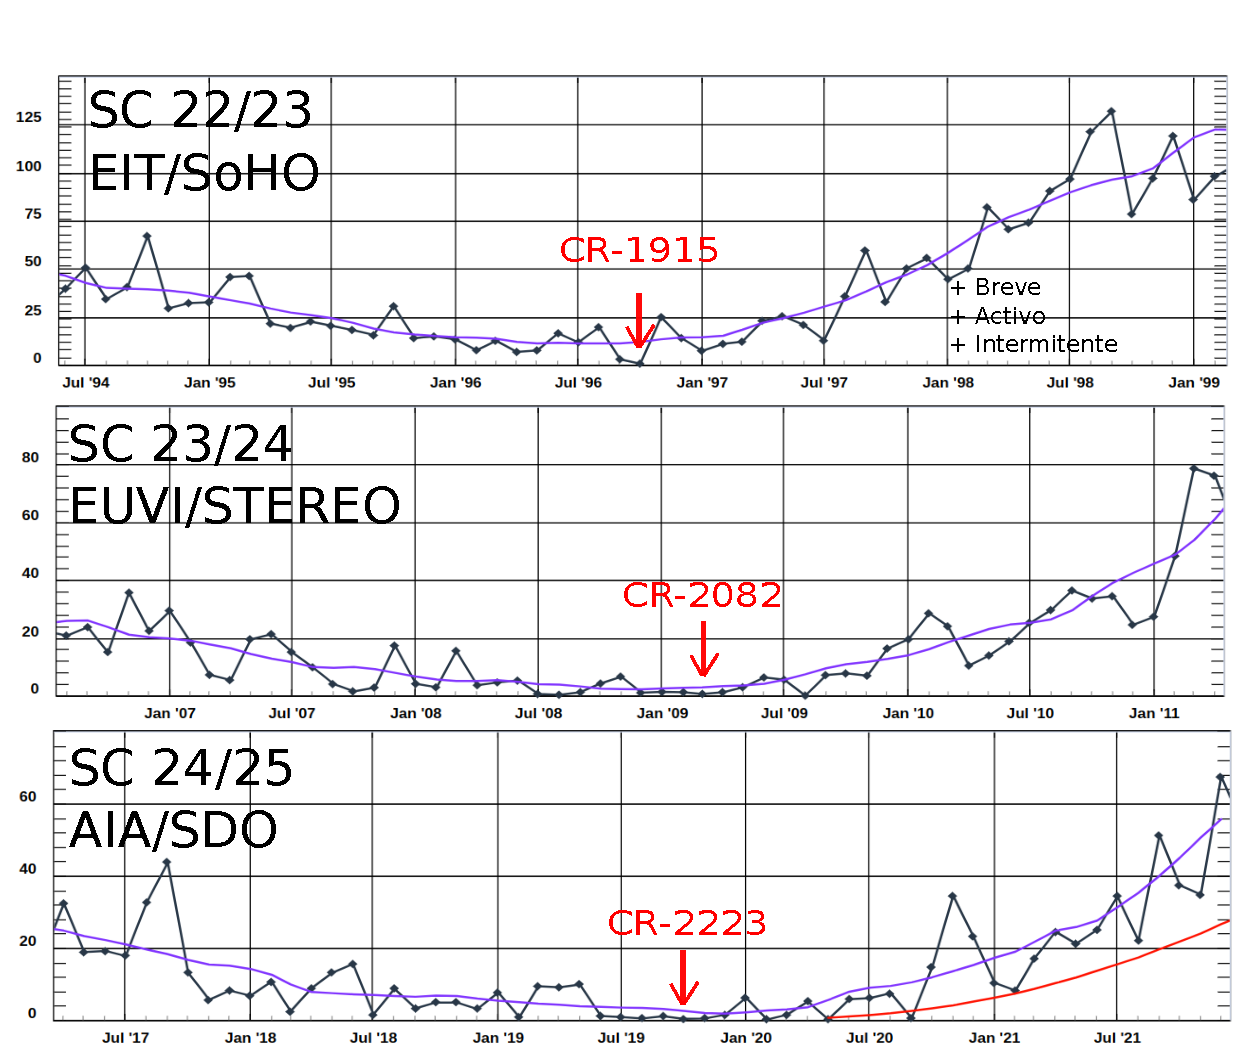
\includegraphics[width=0.99\textwidth,height=0.75\textwidth]{figuras/ciclos_ssn_recorte3.pdf}
\end{center}
%\end{columns}
}

%--------------- Carrmaps
\frame{
\titulo{Reconstrucción DEMT: densidad y temperatura}
\begin{columns}
\column{0.35\textwidth}
\centering
CR-1915 (EIT)\\
$\approx$WSM
\vskip 0.3cm
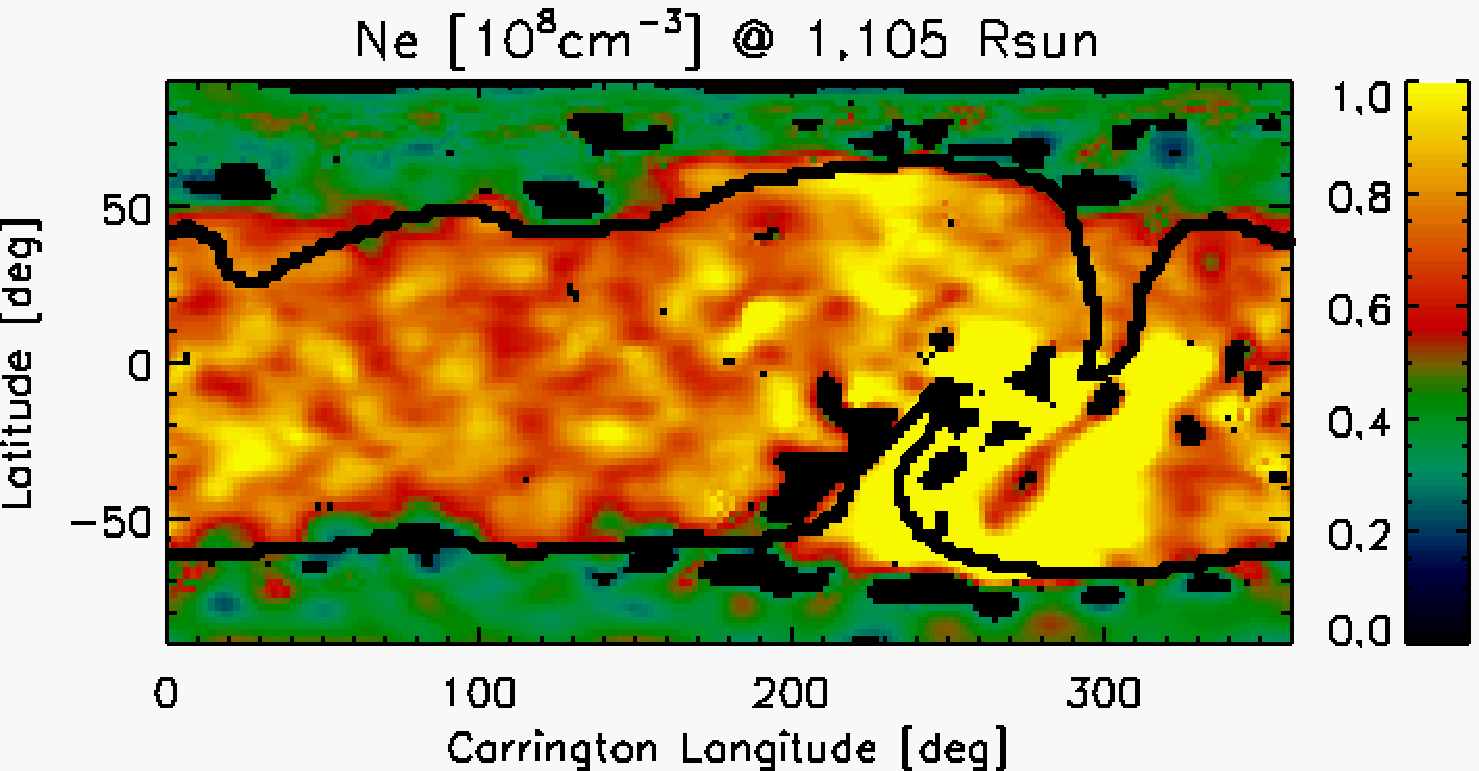
\includegraphics[width=0.95\textwidth,clip=]{figuras/Ne_1105_CR1915.pdf}
\vskip 0.1cm
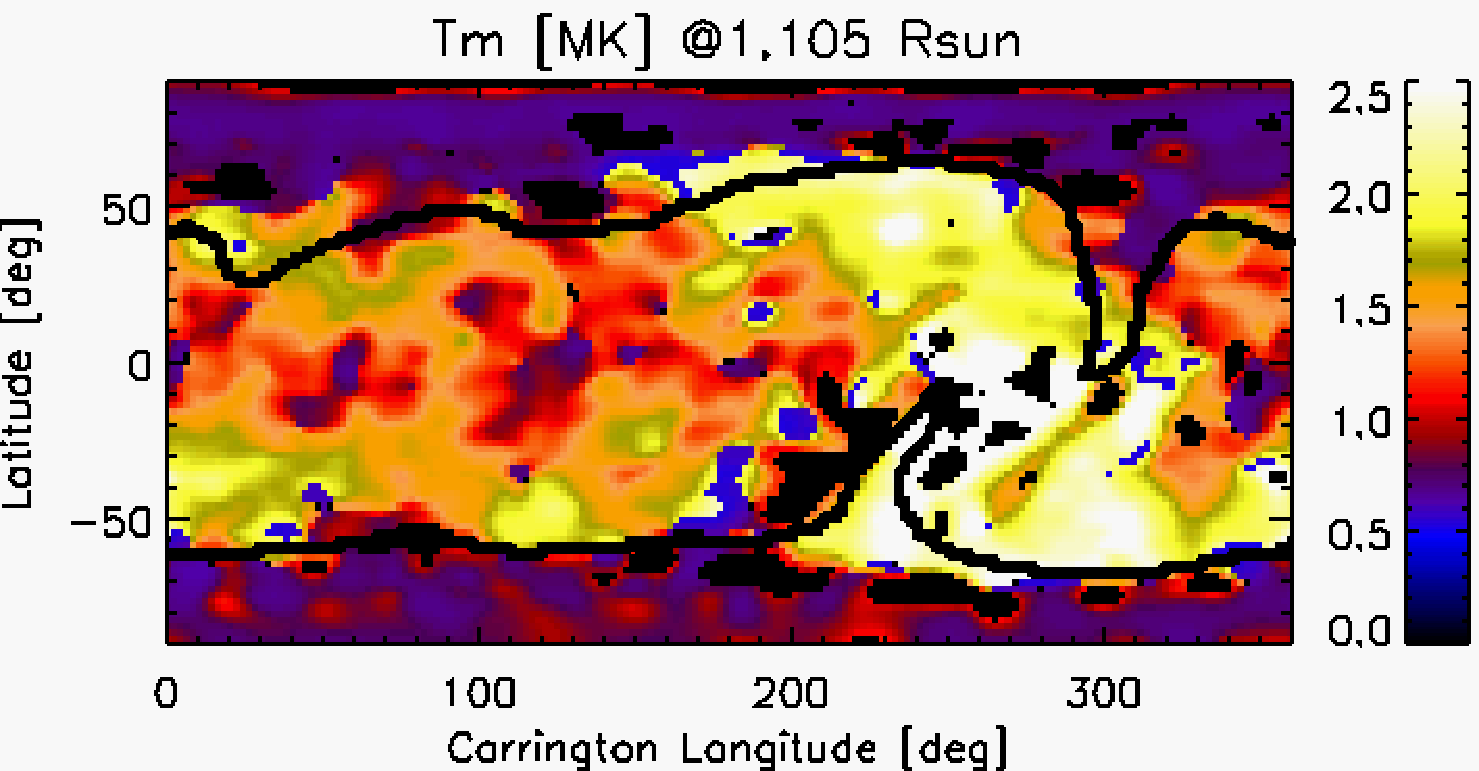
\includegraphics[width=0.95\textwidth,clip=]{figuras/Tm_1105_CR1915.pdf}

%\vskip 0.1cm


\column{0.35\textwidth}
\centering
CR-2081 (EUVI)\\
$\sim$WHI
\vskip 0.3cm
%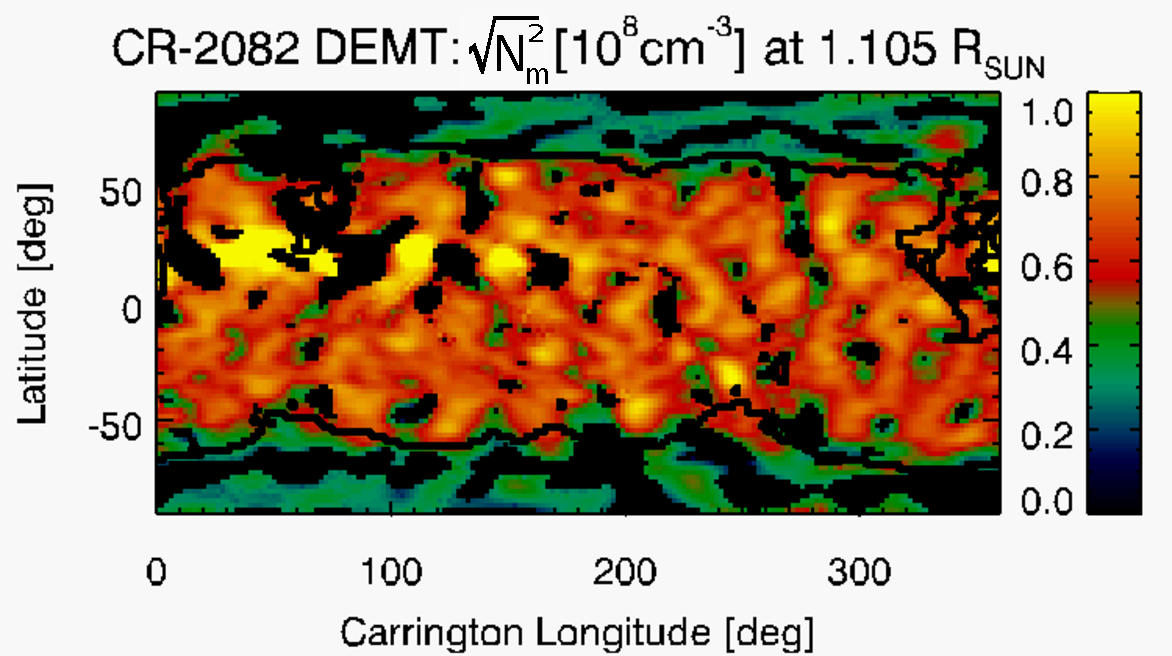
\includegraphics[width=0.95\textwidth]{figuras/map_Ne_CR2082_DEMT-EUVI_behind_H1-L3523_r3d_1105_Rsun.pdf}
%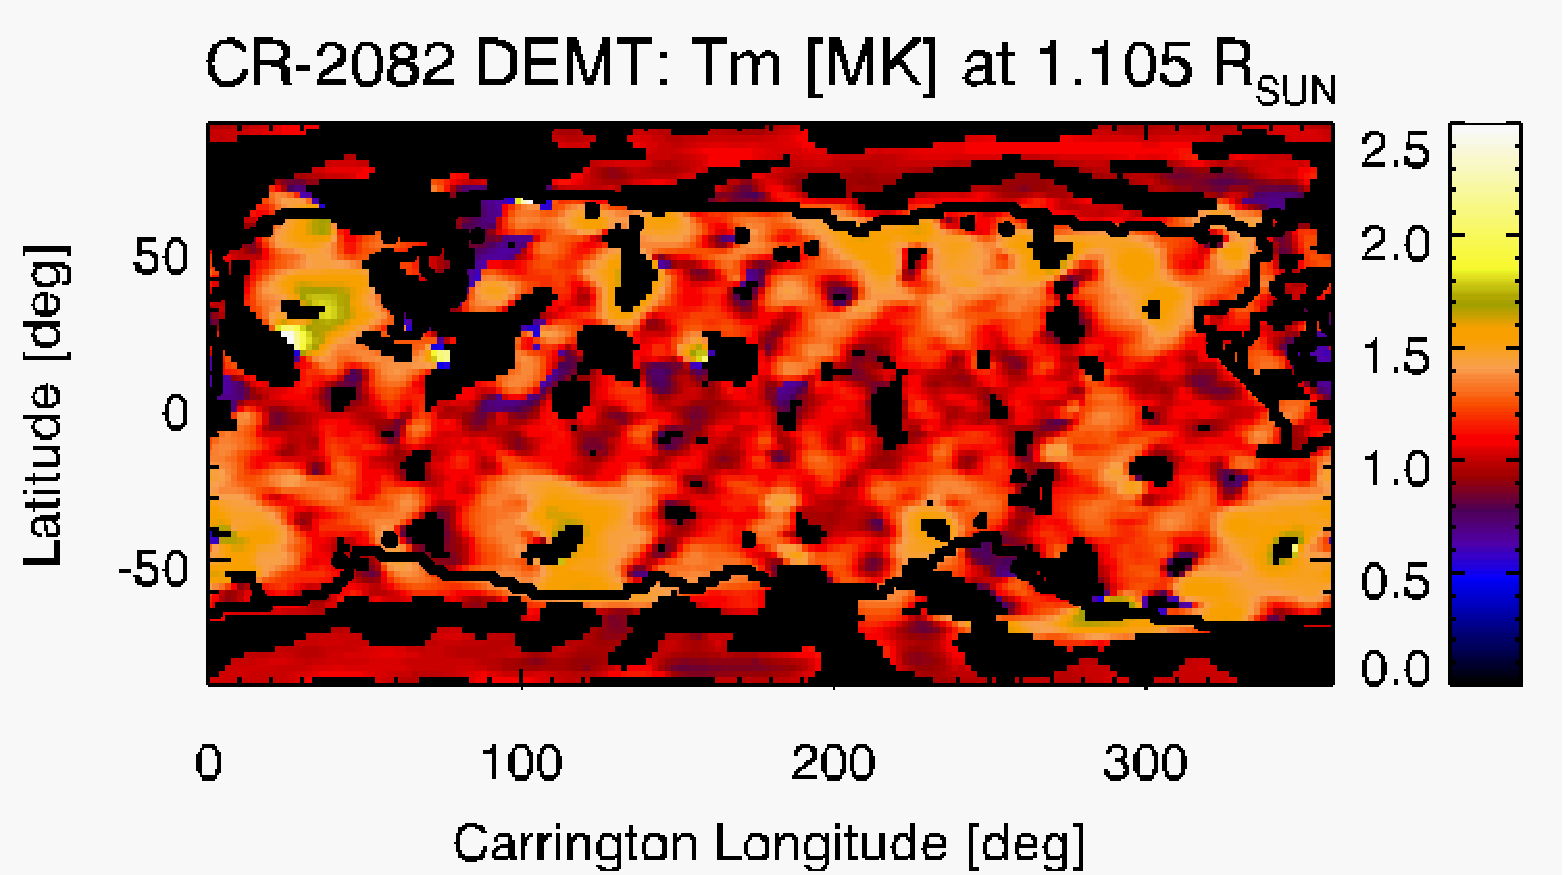
\includegraphics[width=0.95\textwidth]{figuras/map_Tm_CR2082_DEMT-EUVI_behind_H1-L3523_r3d_1105_Rsun.pdf}
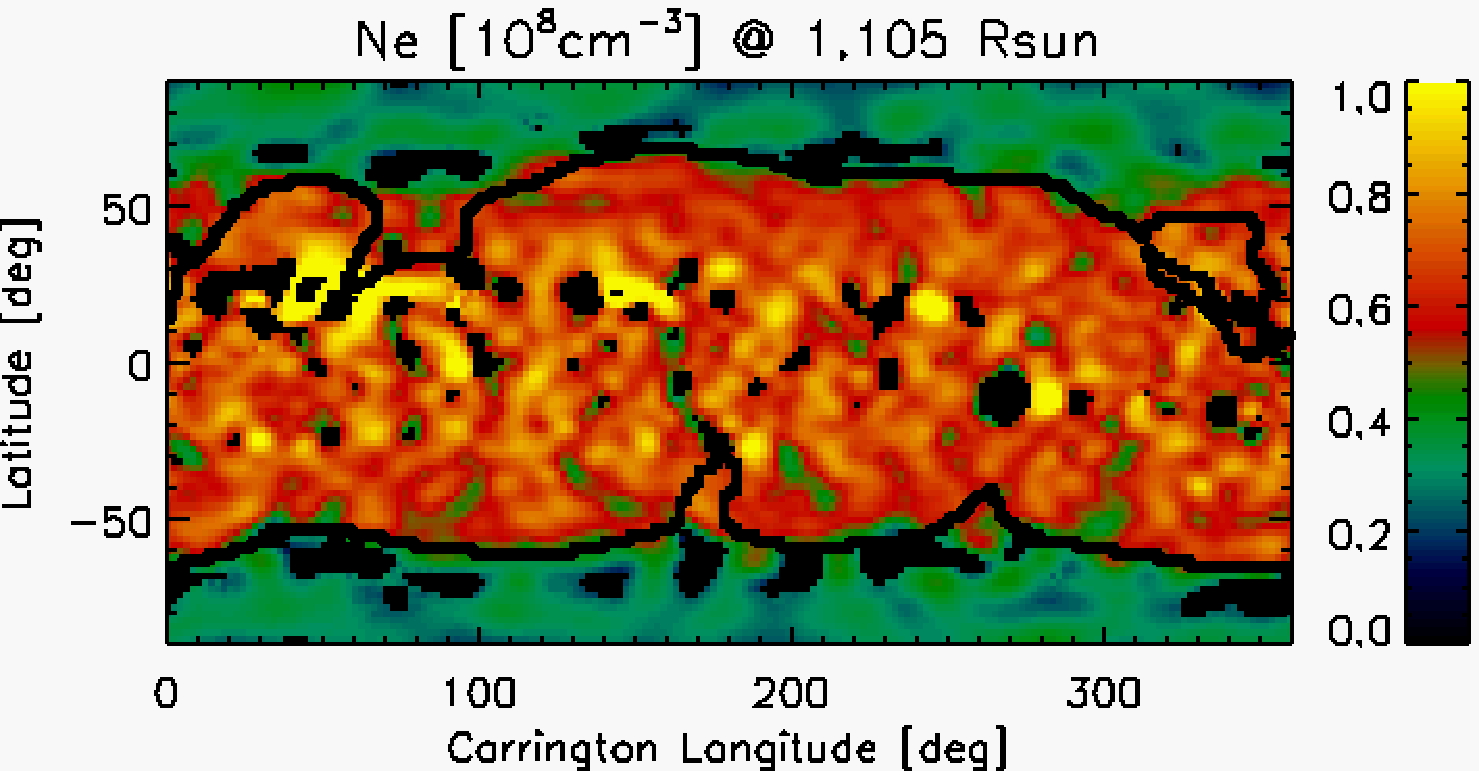
\includegraphics[width=0.95\textwidth]{figuras/Ne_1105_CR2081.pdf}
\includegraphics[width=0.95\textwidth]{figuras/Tm_1105_CR2081.pdf}

\column{0.35\textwidth}
\centering
CR-2223 (AIA)\\
WHPI
\includegraphics[width=0.95\textwidth,clip=]{figuras/map_Ne_CR2223_DEMT-AIA_H1_L733_r3d_multistart_1105_Rsun2223.eps}
\includegraphics[width=0.95\textwidth,clip=]{figuras/map_Tm_CR2223_DEMT-AIA_H1_L733_r3d_multistart_1105_Rsun2223_2.eps}

\end{columns}  
Lloveras et al. (2017,2020,2022)\\
\vskip 0.3cm
\bu Same Azimuthal symmetry\\
\bu Same thermodynamic regions.\\
\bu Good O/C boundary agreement.
}
\end{comment}
%--------------------------------------------------------



\begin{comment}
%-------------------> 
\frame{
\titulo{Corona Solar y la relación Sol-Tierra}
\includegraphics[width=\linewidth]{figuras/Sun-Earth.eps}
\footnotesize
\begin{center}
El estudio observacional y modelado de la atmósfera solar resultan de gran relevancia para la comprensión de la relación Sol-Tierra, siendo esta la región donde el plasma se calienta, el viento solar es acelerado y tienen lugar eventos impulsivos como las erupciones solares y eyecciones coronales de masa.
\end{center}
}

%-------------------
\frame{
\titulo{Estructura solar}
\footnotesize
%\vspace{-0.25cm}
\begin{columns}
\column{0.45\textwidth}
\vspace{0.1cm}

Interior solar\\
\begin{itemize}
\item Núcleo ($r < 0.25\mrsun$, T$\approx 15$MK)
\item Región Radiativa ($0.25\mrsun<r<0.7\mrsun$)
\item Región Convectiva
\end{itemize}
%\vspace{0.15cm}
\begin{center}
\framebox{\includegraphics[width=0.8\textwidth,height=0.9\textwidth]{figuras/interior_solar.png}}
\end{center}
\column{0.55\textwidth}
Atmósfera Solar
\begin{itemize}
\item Fotosfera (T $\approx 6000$K, N $\approx 10^{17}cm^{-3}$)
\item Cromosfera (T $> 6000$K, N $\approx 10^{12}cm^{-3}$)
\item R. Trans. (T $\sim 10^{4-6}$K, N $\sim 10^{11-9}cm^{-3}$)
\item Corona Solar (T $\sim 1$MK, N $\sim 10^{8-9}cm^{-3}$)
\end{itemize}
\begin{center}
\framebox{\includegraphics[width=0.99\textwidth]{figuras/region_transicion.png}}
\end{center}

\end{columns}
}

%-------------------> 
\frame{
\titulo{Ciclo de Actividad Solar y manifestación coronal}
\footnotesize
%\vspace{-0.25cm}
%\begin{itemize}
%  \item El nivel de actividad es medido por cant. de manchas solares y es cíclico (11 años).
%  \item Campo magnético global es fuertemente dipolar (líneas poloidales) en fase de mínimo, e invierte su polaridad cada 11 años.
%  \item Manchas solares y regiones activas (ARs) emergen en latitudes altas y progresan gradualmente hacia el ecuador en forma cíclica cada 11 años.
%  \item Manchas solares emergen de a pares y sus polaridades se alinean conforme a la rotación solar.
%  \item Inclinación de líneas que unen pares de manchas aumenta en latitud.
% \item Ciclos sucesivos con polaridades invertidas (22 años).
%\end{itemize}

\begin{columns}
\column{0.5\textwidth}
\begin{center}
Babcock et al. (1961)\\
\includegraphics[width=0.7\textwidth]{figuras/babckok_model.png}
\end{center}
\column{0.5\textwidth}
\bu Dínamo solar $\rightarrow$ dinámica Solar.\\
\vskip 0.4cm
\bu Mínimo: Dipolo, pocas manchas y ARs.\\
\vskip 0.4cm
\bu Máximo: Multipolo, muchas manchas y ARs.\\
\vskip 0.4cm
\bu Ciclo de 11 años.\\
\end{columns}


%\vspace{-0.55cm}
\begin{center}
%\includegraphics[width=.6\textwidth]{figuras/butterfly-diagram_recorte.pdf}
\includegraphics[width=0.99\textwidth]{figuras/SC_22-25.pdf}
\end{center}
\vskip -0.5cm
Space weather prediction center (NOAA)
}
%----------------------------------------

\frame{
\titulo{Rotaciones analizadas}
\footnotesize
\vspace{-0.8cm}
%\begin{columns}
%\column{0.2\textwidth}
%\centering
%\vspace{-4cm}

%\column{0.8\textwidth}
\begin{center}
\includegraphics[width=0.99\textwidth,height=0.75\textwidth]{figuras/ciclos_ssn_recorte3.pdf}
\end{center}
%\end{columns}
}
%----------------------------------------

\frame{ 
\titulo{Radiación coronal}
\begin{columns}
%\vspace{-1cm}
\column{0.6\textwidth}
\footnotesize
La radiación proveniente de la corona es causada por diversos fenómenos
\begin{itemize}
\item Corona-K: Scattering de Thomson de luz blanca, observable con coronógrafos.
\item Corona-E: Decaimientos electrónicos en iones que emiten en UV, EUV y X.  
\end{itemize}
\salto
\salto

Imágenes EUV de un ciclo solar completo. Imágenes tomadas en la banda ${\rm 195 \AA}$ del instrumento EIT/SoHO.
\begin{itemize}
\item La fase de máximo muestra gran cantidad de ARs y estas aparecen en dos bandas de latitudes bien definidas.
\item La fase de mínimo muestra una marcada disminución de ARs, caracterizando la corona quiescente.
\end{itemize}

\column{0.4\textwidth}
\begin{center}
\azul{Mínimo en luz blanca}
\movie[externalviewer]{\includegraphics[width=0.45\textheight, keepaspectratio]{figuras/streamer_minimo_solar.jpg}}{lasco_2019.mp4}
%\includegraphics[width=0.9\textwidth]{figuras/streamer_minimo_solar.jpg}
%\mediosalto
%\azul{Ciclo en EUV}
%\framebox{\includegraphics[width=0.9\textwidth]{figuras/ciclo_solar.jpg}}
\end{center}
\azul{Ciclo en EUV}
\centering
\movie[externalviewer]{\includegraphics[width=0.45\textheight, keepaspectratio]{figuras/ciclo_solar.jpg}}{2019_AIA_193.mp4}


\end{columns}
}
%----------------------------------------------

\frame{ 
\titulo{Temperaturas características de la corona solar}
\vspace{-.5cm}
\footnotesize
Los telescopios espaciales tienen detectores EUV, cuyos filtros seleccionan principalmente líneas de Fe (T$_e \sim 0.5  - 2.5$ \ MK). \\
%\begin{comment}
%\begin{columns}
% \column{0.5\textwidth}
% Telescopios utilizados:
%\begin{itemize}
% \item Extreme ultraviolet Imaging Telescope (EIT), a bordo de la misión Solar and Heliospheric Observatory (SoHO). Observaciones 1996 - 2006.
% \item Extreme UltraViolet Imager (EUVI), a bordo de las dos naves de la misión Solar TErrestrial Relations Observatory (STEREO). Observaciones 2007 - actualidad. 
% \item Atmospheric imaging Assembly (AIA), a bordo de la misión Solar Solar Dynamic Observatory (SDO). Observaciones 2010 - actualidad. 
%\end{itemize}
%\column{0.5\textwidth}
%\framebox{\includegraphics[width=0.9\textwidth]{figuras/passband_EIT-EUVI.pdf}}
%\includegraphics[height=0.56\textwidth]{figuras/qkl_aia_euvi_test_2.pdf}
%\includegraphics[width=0.99\textwidth]{figuras/qkl_aia_euvi_test_2.pdf}
%\end{columns}
%\end{comment}

\begin{comment}
$$
Q_k(T) \ \ \equiv \ \ \int {\rm d} \lambda \ \ \phi_k(\lambda) \ \ {\eta( N_{e0}, {\bf a}_0,
T; \lambda)} \ / \ {N_{e0}^2}
$$
\vskip 0.2cm
%\begin{columns}
%\column{0.3\textwidth}

%\column{0.7\textwidth}
\includegraphics[height=0.32\linewidth,width=0.3\linewidth]{figuras/panel.eps}
\includegraphics[height=0.35\textwidth,width=0.65\linewidth]{figuras/qkl_aia_euvi_test_2.pdf}
%\end{columns}

%\footnotesize
\bu $\phi_k$: Pasabandas $k$ \hfill Lloveras et al. (2018)\\
%\vskip 0.25cm
\bu $\eta(\lambda,T)$: Modelo de Emisividad CHIANTI.
%\vskip 0.25cm
%\bu EUVI/EIT: ${\bf a}_0 =$ [Fe]\\
%Feldman et al. (1992)
}


%\includegraphics[width=0.32\textwidth]{figuras/1996_11_08_19_12_18_EIT_195.png}
%\includegraphics[width=0.32\textwidth]{figuras/2009_03_16_23_40_05_EUVI-A_195.png}
%\includegraphics[width=0.32\textwidth]{figuras/2019_09_07_05_30_00_AIA_193.png}

%------------------------------
\begin{frame}
\titulo{¿Que es la Tomografía Solar?}
\footnotesize
\vskip 0.1cm
%\rojo{\bf Unknown:} \rojo{3D distribution of a certain quantity $bx_i$} (e.g. $N_e$) for each cell volume $i$ within an object (e.g. the solar corona), under optically thin regime (e.g. coronal white light)\\
\rojo{\bf Incógnita:} \rojo{Distribución en 3D de una determinada cantidad $\bx_i$} (por ejemplo, $N_e$) para cada volumen de celda $i$ dentro de un objeto (p. ej., la corona solar), en régimen óptico delgado (p. ej., luz blanca coronal)

\vskip 0.1cm
\azul{\bf Dato:} 
\begin{itemize} 
%\item \azul{Intensity vector $by_j$:} measurement in each \azul{pixel $j$} of each image of a time-series providing different view angles.\\
\item \azul{Vector de intensidad $\by_j$:} medición en cada \azul{pixel $j$} de cada imagen de una serie temporal proporcionando diferentes ángulos de visión.\\

%\item \azul{\emph{Proyection} matrix $bA_{ji}$:} depending on the \azul{geometry} (e.g. solar rotation, telescope orbit) and the involved \azul{physical process} (e.g. Thomson scatt.).

\item \azul{Matriz de proyección $\bA_{ji}$:} depende de la \azul{geometría} (p. ej., rotación solar, órbita del telescopio) y el \azul{proceso físico} involucrado (p. ej., Thomson scatt.).

\begin{center}
{\includegraphics[width=0.55\linewidth]{figuras/tom_sketch.eps}}
\end{center}
\item \azul{Tomografía rotacional solar}: la rotación solar proporciona los ángulos de visión necesarios.
%\item \azul{$bA$} is a very large sparse matrix, 
% \emph{global optimization} of \emph{objective function}:
%$$
%f(\rojo{{\bf x}}) \ \ =  \ \  
%\| \azul{\by} - \azul{\bA\,\cdotp\,} \rojo{{\bf x}} \|^2 \ \ + \ \
%{\sf regularization\ terms}
%$$
\end{itemize}
\end{frame}




%----------------------------------------------------------------------
\frame{
\titulo{Tomografía Solar Rotacional}
\vskip -0.5cm
\footnotesize
\begin{center}
La señal recibida en el j-ésimo pixel de la k-ésima banda viene dado por\\
$\azul{Y_{k,j}} \ \ = \ \ \azul{ \int_{\mathrm{LDV}} \mathrm{d}l} \  
\azul{A({\bf r}_j(l))} \, \rojo{X \left(k,\azul{{\bf r}_j(l)}\right)} 
\ \ \rightarrow \ \
\azul{\boldsymbol{Y}_k} = \azul{\boldsymbol{A}_k\,\cdotp\,} \rojo{{\boldsymbol{X} }_k} $
\end{center}

\begin{columns}
 \column{0.5\textwidth}

\begin{itemize}
\item Luz Blanca (C2-SRT)
\end{itemize}

$ \rojo{X \left(k,\azul{{\bf r}_j(l)}\right)} = \rojo{N_e}(\azul{{\bf r}_j(l))}$ \\
$ \azul{A({\bf r}_j(l))} =$ factor de scattering Thomson\\
\ \\
\ \\
Se discretiza el volumen, $2.5 - 8.5$ \rsun.\\
\azul{\# Celdas:} $\azul{I}\,=\,60\times60\times120\sim\ \azul{4\times10^5}$
Tamaño típico:\ \ 0.1\,\rsun\,$\times$ 3\deg $\times$ 3\deg \\%\ $\sim$ \ $7\times10^3$km $\times$
\azul{\# Pixels:} $\azul{J}\,=\,512^2\times14\times0.7\sim\ \azul{2.5\times10^6}$


\column{0.5\textwidth}
\begin{itemize}
\item EUV (DEMT)
\end{itemize}


$ \rojo{X \left(k,\azul{{\bf r}_j(l)}\right)} = \rojo{FBE_K}(\azul{{\bf r}_j(l))}$\\
$ \azul{A({\bf r}_j(l))} = 1$\\
donde $\rojo{FBE_K({\bf r})} \equiv \int_{0}^{\infty} \mathrm{d} \lambda \ \phi_k(\lambda)\ \eta ( {\bf r}, \lambda )$\\
\ \\
Se discretiza el volumen, $1.0 - 1.3$ \rsun.\\
\azul{\# Celdas:} $\azul{I}\,=\,30\times90\times180\sim\ \azul{4\times10^5}$
Tamaño típico:\ \ 0.01\,\rsun\,$\times$ 2\deg $\times$ 2\deg \\%\ $\sim$ \ $7\times10^3$km $\times$
\azul{\# Pixels:} $\azul{J}\,=\,512^2\times3\times27\sim\ \azul{2\times10^7}$
\end{columns} 

\begin{center}
 \azul{\ $\boldsymbol{Y}_k$}: Vector de \azul{$J$} elementos, los pixels de todas las imágenes.\\
 \azul{\,$\boldsymbol{A}_k$}: Matriz de \azul{$J\times I$} elementos, puramente geométricos.\\
 \rojo{\,$\rojo{\boldsymbol{X}}_k$}: Vector de \azul{$I$} elementos.
\end{center}

%\vskip 1.cm
\begin{center}
%  Solución: optimización global de función objetivo
Problema de optimización multidimensional. Función objetivo:\\
$f(\rojo{\boldsymbol{X}_k}) = \| \azul{\boldsymbol{Y}_k} - \azul{\boldsymbol{A}_k} \rojo{\boldsymbol{X}}_k   \|^2 + 
 p\ \|  \azul{\bR} \rojo{\boldsymbol{X}}_k   \|^2 \, $
\end{center}

%\begin{columns}
%\column{0.5\textwidth}
%Producto: Ne 3D
%\column{0.5\textwidth}
%Producto: FBE 3D por banda
%\end{columns}

}


%-------------------> FBE + mamuschkas

\frame{ 

\vspace{-0.35cm}
\begin{columns}
\noindent
\column{0.075\textwidth}
\vskip 0.8cm
{\footnotesize
\ 171 \AA
\vskip 1.75cm
\ 195 \AA
\vskip 1.65cm
\ 284 \AA
}
\column{\textwidth}
\begin{center}
{\footnotesize
\ \ Imágenes Dato \hfill $\rightarrow$ \hfill 3D FBE \hfill $\rightarrow$ \hfill Imágenes Sintéticas\ \ \ \
}\\
\framebox{\includegraphics[width=0.95\linewidth]{figuras/frame_050_test.pdf}}\\
\footnotesize
 1.035 $\mrsun$ \hskip 1cm 1.085 $\mrsun$ \hskip 1cm 1.135 $\mrsun$ \hfil
\end{center}
\end{columns}
\begin{columns}
 \column{0.4\textwidth}
 Vásquez et al. (2009)
 \column{0.6\textwidth}
\end{columns}
}


%----------------------------------- LDEM

\frame{
\titulo{Medida de Emisión Diferencial local (LDEM)}
\footnotesize
\begin{itemize}
\item
En cada celda tomográfica \azul{$i$} se conocen K \azul{FBEs}.
\salto
\item
Utilizando las Respuestas Térmicas \azul{$Q_k(T)$}
\salto
\item
Las FBEs pueden reescribirse como:
$\azul{FBE_{k,i} } \, = \, \azul{\int \mathrm{d}T \  Q_k(T) \ \, \rojo{{\sf LDEM}_i(T)} }$.
\salto
\item
Donde la \rojo{${\sf LDEM}_i(T)$ [cm$^{-6}$K$^{-1}$]} para cada celda \azul{$i$} se define tal que:
\begin{eqnarray}
N_{m,i}^2 = \left< N_e^2\right>_i &=& \int \mathrm{d} T \ \, \rojo{{\sf LDEM}_i(T)}\nonumber\\
T_{m,i} = \left<T_e\right>_i  &=& \frac{1}{\left< N_e^2\right>_i } \int \mathrm{d}T\ T \ \, \rojo{{\sf LDEM}_i(T)}\nonumber \\
 W_{T,i}^2 &=&  \frac{1}{\left< N_e^2\right>_i} \int_{T_{min}}^{T_{max}} dT\ \rojo{{\sf LDEM}_i(T)}\ (T - \langle T_e \rangle_i)^2 \nonumber
\end{eqnarray}
%\salto
\item Se modela la LDEM:\ 
$\rojo{{\sf LDEM}_i(T)}=\azul{\mathcal{N}(}T,\,\rojo{\mathbf{\lambda}_i=[A,T_0,\sigma_T]}\azul{)}$ Nuevo et al. (2015)
\salto
\item
La siguiente función objetivo es minimizada en cada celda: \mediosalto
\hskip 3cm
$
\Phi(\rojo{{\mathbf{\lambda}}_i}) \ = \ 
\ \azul{\sum_{k}}| \ \azul{ FBE_{k,i} }-
\azul{\int \mathrm{d}T \ \, Q_k(T)\ \, \mathcal{N}(T,}\,\rojo{\mathbf{\lambda}_i}\azul{)} \ 
|^2 
$.
\item Grado de éxito 
$
R_i \equiv (1/K) \sum_{k} | 1 - { FBE_{k,i} } / {\int \mathrm{d}T \ \, Q_k(T)\ \, \mathcal{N}(T,}\,{\mathbf{\lambda}_i}{)} |
$
\end{itemize}
}


%--------------------------
\frame{
\titulo{LDEM características}
\begin{center}
\includegraphics[width=0.495\textwidth,clip=]{figuras/Nueva_figura_paper_LDEM_2.eps}
\includegraphics[width=0.495\textwidth,clip=]{figuras/Nueva_figura_paper_3.eps}
\end{center}

\begin{columns}
  
\column{0.5\textwidth}
%Lloveras et al. (2022)
\begin{center}
\includegraphics[width=0.99\textwidth,clip=]{figuras/R_1025_CR2081.pdf}
\end{center}

\column{0.5\textwidth}
\hfill Lloveras et al. (2022)\\

\vskip 2cm
$R \sim 1\% \, (Streamer) \, y \sim 10\% \, (CHs)$

\end{columns}
}





%--------------- Carrmaps
\frame{
\titulo{Reconstrucción DEMT: densidad y temperatura}
\begin{columns}
\column{0.35\textwidth}
\centering
CR-1915 (EIT)
\vskip 0.3cm
\includegraphics[width=0.95\textwidth,clip=]{figuras/Ne_1105_CR1915.pdf}
\vskip 0.1cm
\includegraphics[width=0.95\textwidth,clip=]{figuras/Tm_1105_CR1915.pdf}

%\vskip 0.1cm


\column{0.35\textwidth}
\centering
CR-2081 (EUVI)
\vskip 0.3cm
%\includegraphics[width=0.95\textwidth]{figuras/map_Ne_CR2082_DEMT-EUVI_behind_H1-L3523_r3d_1105_Rsun.pdf}
%\includegraphics[width=0.95\textwidth]{figuras/map_Tm_CR2082_DEMT-EUVI_behind_H1-L3523_r3d_1105_Rsun.pdf}
\includegraphics[width=0.95\textwidth]{figuras/Ne_1105_CR2081.pdf}
\includegraphics[width=0.95\textwidth]{figuras/Tm_1105_CR2081.pdf}

\column{0.35\textwidth}
\centering
CR-2223 (AIA)
\includegraphics[width=0.95\textwidth,clip=]{figuras/map_Ne_CR2223_DEMT-AIA_H1_L733_r3d_multistart_1105_Rsun2223.eps}
\includegraphics[width=0.95\textwidth,clip=]{figuras/map_Tm_CR2223_DEMT-AIA_H1_L733_r3d_multistart_1105_Rsun2223_2.eps}

\end{columns}  
Lloveras et al. (2017,2020,2022)\\
\vskip 0.3cm
\bu Simetría acimutal\\
\bu Streamer(CHs) $\rightarrow$ mayor(menor) densidad y temperatura.\\
\bu Gradientes máximos en frontera A/C
}



%------------------- PFSS

\frame{
\titulo{Visualización 3D del modelado magético PFSS}
\begin{columns}

%\column{0.3\textwidth}
%\centering Magnetograma
%\includegraphics[width=0.99\textwidth]{figuras/magnetograma_esferico2.jpg}

%\column{0.3\textwidth}
%\centering Magnetograma sinóptico
%\includegraphics[width=0.99\textwidth]{figuras/mrmqj090419t1341c2082_000.jpg}

\column{0.5\textwidth}
\centering 
Magnetograma sinóptico\\
\includegraphics[width=0.99\textwidth]{figuras/fig1_nishtha2019_gong.pdf}\\
\includegraphics[width=0.99\textwidth]{figuras/fig1_nishtha2019_adapt_gong.pdf}

%\column{0.4\textwidth}
\column{0.5\textwidth}
\centering Modelo potencial
\includegraphics[width=0.99\textwidth]{figuras/CR2081.jpg}
\end{columns}
\bu \small{ADAPT: modelo de transporte de flujo magnético.}

%\begin{align}
% \nabla \cdot B = \nabla \cdot (\nabla \Phi) & = 0  \nonumber \\
% \frac{\partial \Phi}{\partial r} (r=1\mrsun,\theta,\phi) & = M(\theta,\phi) \nonumber\\ 
% \Phi(r=R_{ss},\theta,\phi) & = 0 \nonumber
%\end{align}

\vskip -0.2cm
\begin{columns}
\column{0.2\textwidth}
\column{0.3\textwidth}
$\nabla \cdot B = \nabla \cdot (\nabla \Phi)  = 0$
\column{0.3\textwidth}
\begin{equation*}
\left\lbrace
  \begin{array}{l}
%\begin{align}
 %\nabla \cdot B = \nabla \cdot (\nabla \Phi) & = 0 \nonumber \\
 \frac{\partial \Phi}{\partial r} (r=1\mrsun,\theta,\phi)  = M(\theta,\phi) \nonumber \\
 \Phi(r=2.5\mrsun,\theta,\phi)  = 0 \nonumber
%\end{align}
\end{array}
\right.
\end{equation*}
\column{0.2\textwidth}
\end{columns}
}


%----------------Trazado - Ajuste DEMT

\frame{ 
\vspace{-0.35cm}
\titulo{Trazado y ajuste en líneas magnéticas}
\footnotesize
\begin{columns}
\column{0.6\textwidth}
\begin{itemize}
\item Reconstrucción geométrica de líneas 
\item Puntos de arranque cada 2\deg $\times$ 2\deg $\times$ 10 alturas
\item Trazado de DEMT a lo largo de líneas magnéticas 
\item Se realizan ajustes de densidad y temperatura a lo largo de las líneas
\end{itemize}
\column{0.4\textwidth}
{\includegraphics[width=\textwidth]{figuras/loop_R.jpg}}
\end{columns}
\vspace{0.25cm}
\begin{columns}
\column{0.5\textwidth}
{\includegraphics[width=\textwidth]{figuras/loop_Ne2.jpg}}
$$ N_e = N_0\, \exp{[-(h/\l)/(r/\mrsun)]}$$
\column{0.5\textwidth}
{\includegraphics[width=\textwidth]{figuras/loop_T2.jpg}}
$$\hfill \ \ \ \ \ \ \ \ T_m = ar + b$$
\end{columns}

\vskip 0.3cm
\begin{columns}
\column{0.7\textwidth}
\column{0.3\textwidth}
\rojo{UP} \, \, \,  $(a \equiv \dTm_dr>0)$\\
\azul{DOWN} $(a \equiv \dTm_dr<0)$
\end{columns}
}

%-----------------------------

\frame{
\titulo{Criterio de selección de líneas}



\footnotesize
\begin{itemize}
\item Atravesar al menos cinco celdas de la grilla tomográficas con datos reconstruidos y debe haber al menos un dato en cada tercio del rango de alturas que abarca la {línea, a fin de garantizar un muestreo de alturas completo.}

\vskip 0.7cm
\item La correlación entre la temperatura DEMT y la altura {debe} cumplir $|\rhoTr| > 0.5$. \\
\bu \rojo{UP} \, \, \,  $\rhoTr > 0.5$\\
\bu \azul{DOWN} $\rhoTr < 0.5$

\vskip 0.7cm
\item Test chi-cuadrado para evaluar la bondad del ajuste, seleccionando aquellas líneas donde el nivel de confianza de los ajustes son superior al 90\%.
\end{itemize}


}

%------------------->  Rpint y regiones

\frame{ 
\footnotesize
\vspace{-0.05cm}
\titulo{Regiones coronales analizadas}
%\titulo{Localización de líneas magnéticas y sub-regiones}



\begin{columns}
\column{0.5\textwidth}
\begin{tabular}{c c c c c}
\hline
  Línea  & Característica  &  Latitud Basal   \\
\hline
   0   & \azul{Cerrada  Chica Down} &  $|\theta_0|<50^\circ$  \\
   I   & \orange{Cerrada  Chica Up} &  $|\theta_0|<50^\circ$  \\
   II  & \rojo{Cerrada  Grande Up}   &  $|\theta_0|>40^\circ$  \\
   III & \cian{Abierta  Grande Up}   &  $|\theta_0|>60^\circ$  \\
\hline
\end{tabular}
\column{0.5\textwidth}
%\includegraphics[width=0.95\textwidth,clip=]{figuras/Grispoint_2082_demt_paper_test_Rpoint-map.pdf}
\includegraphics[width=0.99\textwidth,clip=]{figuras/histo_cr2082_full_conajuste_doble_errorhighpoints.eps}
\end{columns}

\begin{center}
\includegraphics[width=0.49\textwidth,clip=]{figuras/Grispoint_2082_demt_paper_test_Rpoint-map.pdf}
\includegraphics[width=0.49\textwidth,clip=]{figuras/Highpoint_2082_demt_paper_cr2082_full_conajuste_doble_error_Rpoint-map.pdf}
\end{center}


}
%---------------------------

\frame{ 
\titulo{Comparación estadística por regiones}

\begin{columns}
\column{0.4\textwidth}
\azul{CR-2082} \\
\rojo{CR-2208}
\vskip 2cm
\bu Streamer (T0 $\rightarrow$ TII):\\
$N_{CB}$ decrece; $\lambda_N$ y $\left<T_m\right>$ crece. \\


\bu CHs (T III): \\
$N_{CB}$, $\lambda_N$ y $\left<T_m\right>$ decrecen.


\column{0.6\textwidth}
\begin{center}
\includegraphics[width=0.32\textwidth,clip=]{figuras/histo_2082_2208_fulldemt_streamer_down_ne_1055.eps}
\includegraphics[width=0.32\textwidth,clip=]{figuras/histo_2082_2208_fulldemt_streamer_down_lambda_n.eps}
\includegraphics[width=0.32\textwidth,clip=]{figuras/histo_2082_2208_fulldemt_streamer_down_Tm.eps}\\
\includegraphics[width=0.32\textwidth,clip=]{figuras/histo_2082_2208_fulldemt_streamer_up_ne_1055.eps}
\includegraphics[width=0.32\textwidth,clip=]{figuras/histo_2082_2208_fulldemt_streamer_up_lambda_n.eps}
\includegraphics[width=0.32\textwidth,clip=]{figuras/histo_2082_2208_fulldemt_streamer_up_Tm.eps}\\
\includegraphics[width=0.32\textwidth,clip=]{figuras/histo_2082_2208_fulldemt_bound_up_ne_1055.eps}
\includegraphics[width=0.32\textwidth,clip=]{figuras/histo_2082_2208_fulldemt_bound_up_lambda_n.eps}
\includegraphics[width=0.32\textwidth,clip=]{figuras/histo_2082_2208_fulldemt_bound_up_Tm.eps}\\
\includegraphics[width=0.32\textwidth,clip=]{figuras/histo_2082_2208_fulldemt_CH_up_conajustene_1055.eps}
\includegraphics[width=0.32\textwidth,clip=]{figuras/histo_2082_2208_fulldemt_CH_up_conajustelambda_n.eps}
\includegraphics[width=0.32\textwidth,clip=]{figuras/histo_2082_2208_fulldemt_CH_up_conajusteTm.eps}
\end{center}

\end{columns}

}
%----------------------
\frame{
\titulo{Barras de Error en DEMT}
\footnotesize
\begin{itemize}
\item Determinación del nivel de regularización de la inversión tomográfica de las emisividades de cada banda.
\salto
\item Incerteza en la calibración radiométrica de las emisividades de cada banda (debido a factores instrumentales):
\begin{itemize}
\item Absoluta $\longrightarrow$ común a las tres bandas. Implica cambio de amplitud en la LDEM $\longrightarrow$ solo modifica ${\rm N_e}$
\salto
\item Relativa $\longrightarrow$ referido diferencia de intensidad medida por las 3 bandas en un pixel y modifica cada banda por separado.
\end{itemize}

\item Propagación de errores: \azul{$\Delta T_m \lesssim 5\%$} y \azul{$\Delta N_m \lesssim 10\%$}  
\end{itemize}
}

%--------------------------------------------------------
\frame{ 
\titulo{Conclusiones DEMT}

%conclusion DEMT de comparacion de 3 mínimos. \\
\footnotesize


\btr Características generales:\\
\bu Los Streamers exhiben $N_{CB} \approx 1.0-1.2\times 10^8\,{\rm cm}^{-3}$, los CHs se caracterizan por una densidad del orden de la mitad. \\
\vskip 0.2cm
\bu $\lambda_N \approx 7-11\times 10^{-2}\,\mrsun$, con los valores menores correspondiendo a las latitudes más bajas del streamer y a los CHs. \\
\vskip 0.2cm
\bu Los streamers se caracterizan por $\left<T_m\right>\approx 1.2-1.6$~MK (con las temperaturas menores correspondiendo a las latitudes más bajas) mientras que los CHs exhiben $T_{m} \lesssim 1$~MK.\\
\vskip 0.2cm
\bu Hallamos la presencia de loops down en los 3 mínimos. Nuevo et al. (2013); Schiff and Cranmer (2016). Presenta condicionamiento al modelo de calentamiento coronal.\\
%Correlación entre número de líneas tipo 0 y mínimo de actividad.\\
%$\beta > 1$ favorece la conversión de ondas de Alfvén en modos compresibles.\\

\vskip 0.7cm
\btr Comparación de los últimos 3 mínimos:\\
\bu $\left<T_m^{SC \, 22/23}\right>  > \left<T_m^{SC \, 23/24}\right>  \lesssim \left<T_m^{SC \, 24/25}\right> $\\
\vskip 0.2cm
\bu $N_{CB}^{SC \, 22/23} > N_{CB}^{SC \, 23/24} > N_{CB}^{SC \, 24/25}$\\
\vskip 0.2cm
\bu SC 22/23 fue el mas breve, activo e intermitente en su nivel de actividad, seguido por SC 23/24 y SC 24/25.\\
%\vskip 0.1cm
%\bu \# Loops down máximo durante SC 23/24.

}


%----------------------

\frame{ 
\titulo{Space Weather Modeling Framework}
\begin{columns}
\column{0.7\textwidth}
\includegraphics[width=0.99\textwidth]{figuras/oran_2015.png}
\column{0.3\textwidth}

\scriptsize
\bu Desarrollado en CLaSP de la Univ. de Michigan\\
\vskip 0.5cm
\bu Modela sist. Sol-Hel-MI\\
\vskip 0.5cm
\bu Vasto rango de escalas espacio-temporales
\vskip 0.5cm
\bu Código Modular \\
\vskip 0.5cm
\bu AWSoM: SC y IH\\


\end{columns}
}

%----------------------
\frame{ 
\titulo{Modelo MHD de la corona global (AWSoM)}
%\vspace{-0.5cm}
\footnotesize

\bu Cond. de contorno ADAPT-GONG $\rightarrow$ PFSS\\
\bu Región de Transición extendida\\
\bu Conserv. masa, inducción, divergencia nula \\


%\end{itemize}

%\scriptsize
\vskip 0.2cm
%\begin{equation}
\bu Conserv. del momento:\\

$\frac{\partial}{\partial t}(\rho \vec{v}) + \nabla \cdot \left[ \rho \vec{v}\vec{v} + (p_i +p_e +\azul{p_A}+\frac{1}{2\mu_0}B^2) \vec{I} - \frac{\vec{B}\vec{B}}{\mu_0} \right] = - \rho \frac{GM_{\odot}}{r^3} \vec{r} $
%\end{equation}

\vskip 0.5cm
\bu Ecuaciones de energía:\\
%\begin{equation}
%\begin{split} 
$\frac{\partial}{\partial t} \Bigg( \frac{1}{2}\rho v^2 + \frac{p_i}{\gamma -1} +\frac{1}{2} B^2 \Bigg) +  \nabla \cdot  \left[ \Bigg( \frac{1}{2} \rho v^2 + \frac{ \gamma p_i}{ \gamma -1} + B^2 \Bigg) \vec{v} -\vec{v}\cdot  \vec{B}\vec{B}  \right] =  \frac{N_i k_b}{\tau_{ei}}(T_e - T_i) + \rojo{Q_i} $

%-\rho \frac{GM_{\odot}}{r^3}\vec{r}\vec{v}
  %\nonumber
%\end{split}
%\end{equation}

%\begin{equation}
%\begin{split} 
\vskip 0.5cm
$ \frac{\partial}{\partial t} \Bigg( \frac{p_e}{\gamma -1} \Bigg) +  \nabla \cdot \Bigg( \frac{\gamma p_e}{\gamma -1}\vec{v} \Bigg) + \nabla \cdot \Bigg( \azul{p_A} \vec{v} \Bigg) =
  -\nabla \cdot \vec{q_e} +\frac{N_i k_b}{\tau_{ei}}(T_i - T_e) -Q_{rad} + \rojo{Q_e} $
%\end{split}
%\end{equation}

%\begin{equation}
\vskip 0.5cm
\bu Densidad de energía de ondas de Alfvén:
$  \frac{\partial w_\pm}{\partial t} + \nabla \cdot [(\boldsymbol{v}\pm \boldsymbol{V}_A)w_\pm] = - \frac{w_\pm}{2}(\nabla \cdot \boldsymbol{v}) \verde{- \Gamma_{\pm} w_\pm \mp R\sqrt{w_- w_+}}$  %\nonumber
%\end{equation}



$\Gamma_{\pm} = \frac{2}{L}\sqrt{\frac{w_{\mp}}{\rho}}$ Dmitruk et. al (2002)  \, \, $\rojo{Q_i} + \rojo{Q_e} = \Gamma_+w_+ + \Gamma_-w-$   \, \, $\azul{p_A} = (w_+ + w_-)/2$


van der Holst et al. (2014) \hfill Sachdeva et al. (2019,2021); Lloveras et al. (2022)

}


%----------------------
\frame{ 
\titulo{DEMT vs. AWSoM}
\scriptsize
\bu Objetivo: Validar la capacidad del modelo en reproducir las reconstrucciones.
%\bu Motivación: Es AWSoM capaz para reproducir las reconstrucciones tomográficas?
\vskip -0.2cm
\begin{center}
\includegraphics[width=0.495\textwidth,clip=]{figuras/map_Ne_CR2223_DEMT-AIA_H1_L733_r3d_multistart_1105_Rsun2223.eps}
\includegraphics[width=0.495\textwidth,clip=]{figuras/map_Tm_CR2223_DEMT-AIA_H1_L733_r3d_multistart_1105_Rsun2223_2.eps}\\
\includegraphics[width=0.495\textwidth,clip=]{figuras/map_Ne_awsom_2223_ener_new_1105_Rsun2223.eps}
\includegraphics[width=0.495\textwidth,clip=]{figuras/map_Te_awsom_2223_ener_new_1105_Rsun2223_2.eps}\\
\end{center}

\bu En general hay buen acuerdo en magnitud y morfología de estructuras.\\
\bu Diferencia en HS.
}

%--------------- imág sintéticas
\frame{
\titulo{DEMT vs AWSoM: Imágenes sintéticas}
\begin{center}
\includegraphics[width=0.99\textwidth,clip=]{figuras/Figura_2_paper_imag_sinteticas_2.eps}
\end{center}
$I_{Synt} \sim \int_{LDV} \mathrm{d}l \, N_e^2 \, Q_k$\\
\vskip 0.2cm
\bu El análisis sugiere que la discrepancia es consecuencia del magnetograma.\\
$\Rightarrow$ filtramos líneas abiertas de alta N$_e$.
}






%----------------------

\frame{ 
\titulo{DEMT vs AWSoM: Comparación por regiones}

\begin{center}
%\includegraphics[width=0.22\textwidth,clip=]{figuras/histo_2223_demt_awsom_type0_ne_1055.eps}
%\includegraphics[width=0.22\textwidth,clip=]{figuras/histo_2223_demt_awsom_type0_lambda_n.eps}
%\includegraphics[width=0.22\textwidth,clip=]{figuras/histo_2223_demt_awsom_type0_Tm.eps}\\
\includegraphics[width=0.24\textwidth,clip=]{figuras/histo_2223_demt_awsom_type1_ne_1055.eps}
\includegraphics[width=0.24\textwidth,clip=]{figuras/histo_2223_demt_awsom_type1_lambda_n.eps}
\includegraphics[width=0.24\textwidth,clip=]{figuras/histo_2223_demt_awsom_type1_Tm.eps}\\
\includegraphics[width=0.24\textwidth,clip=]{figuras/histo_2223_demt_awsom_type2_ne_1055.eps}
\includegraphics[width=0.24\textwidth,clip=]{figuras/histo_2223_demt_awsom_type2_lambda_n.eps}
\includegraphics[width=0.24\textwidth,clip=]{figuras/histo_2223_demt_awsom_type2_Tm.eps}\\
\includegraphics[width=0.24\textwidth,clip=]{figuras/histo_2223_demt_awsom_type3_ne_1055.eps}
\includegraphics[width=0.24\textwidth,clip=]{figuras/histo_2223_demt_awsom_type3_lambda_n.eps}
\includegraphics[width=0.24\textwidth,clip=]{figuras/histo_2223_demt_awsom_type3_Tm.eps}
\end{center}

\bu Streamer (TI $\rightarrow$ TII):
$N_{CB}$ decrece; $\lambda_N$ y $\left<T_m\right>$ crece. \\

\bu CHs (T III): $N_{CB}$, $\lambda_N$ y $\left<T_m\right>$ decrecen.\\

\bu AWSoM no es capaz de modelar loops down.

}
%----------------------
\frame{
\titulo{Diferencias DEMT - AWSoM}

\includegraphics[width=0.45\textwidth,clip=]{figuras/perfil_paper_necr2223_bajo.eps}
\includegraphics[width=0.45\textwidth,clip=]{figuras/perfil_paper_tecr2223_bajo.eps}

%\footnotesize
\vskip 1cm
\bu AWSoM reproduce las densidades basales DEMT con un acuerdo $\lesssim 10\%$. \\
\vskip 0.2cm
\bu La $\lambda_N$ y temperatura simuladas son sistemáticamente $5-20\%$ menores.\\
\vskip 0.2cm
\bu Diferencias $\gtrsim$ que las barras de error de DEMT.\\


%\begin{table}
%\centering
%\begin{tabular}{l r@{.}l@{\hskip 0.05in} r@{\hskip 0.01in} r  r@{.}l@{\hskip 0.05in} r@{\hskip 0.01in} r r@{.}l@{\hskip 0.05in} r@{\hskip 0.01in} r }
%\hline
%Tipo    & \multicolumn{4}{c}{$\med(N_{CB})$}             & \multicolumn{4}{c}{$\med(\lambda_N)$}  & \multicolumn{4}{c}{$\med(\avgTe)$} \\
%        & \multicolumn{4}{c}{$[10^8\,{\rm cm}^{-3}]$}  & \multicolumn{4}{c}{$[10^{-2}\mrsun]$}   & \multicolumn{4}{c}{$[\MK]$} \\
%\hline          
%CR-2223\\
%0    & 1&03 &     &      &   7&3 &    &      &   1&29 &    &      \\
%I    & 0&94 &(\Mi&~3\%)  &   9&4 &(\Mi&11\%) &   1&43 &(\Mi&14\%) \\
%II   & 0&79 &(\Mi&13\%)  &   11&0&(\Mi&13\%) &   1&59 &(\Mi&10\%) \\
%III  & 0&47 &(\Pl&~2\%)  &   9&0 &(\Mi&19\%) &   1&13 &(\Mi&12\%) \\
%\hline  
%\end{tabular}
%\end{table}
}
%--------------------------C2-SRT
\frame{
\titulo{Tomografía LB (C2-SRT) vs. AWSoM}
\begin{center}
\includegraphics[width=0.495\textwidth,clip=]{figuras/map_LASCOC2pB_CR2223_24hr-Cadence_Rmin225_Rmax825_IRmin25_IRmax60_60x60x120_BF2_r3D_l25e-5_vfinal_interpolado_2500_Rsun2223.eps}
\includegraphics[width=0.495\textwidth,clip=]{figuras/map_Ne_awsom_2223_ener_new_2505_Rsun2219.eps}\\
\end{center}

\scriptsize
\bu Buena consistencia general en forma y tamaño de streamer y CHs.
%FoV Lasco-C2: $2.5-6.0\, \mrsun$

\vskip 0.2cm
\includegraphics[width=0.99\textwidth,clip=]{figuras/Figura_7_paper_imag_sintetica_2.eps}

$I_{Synt} \sim \int_{LDV} \mathrm{d}l \, N_e $\
}
%----------------------------------
\frame{
\titulo{Ajuste densidad electrónica}
\footnotesize
%\scriptsize
%\begin{equation}

\bu Rango de alturas grandes $\rightarrow$ ley de potencia.

\begin{center}
$N_e^{\rm (C2-SRT)}(r) = N_0\,\left(\,r/2.5\,\mrsun\right)^{-p} \rightarrow  \langle \l \rangle \equiv  \left\langle \left|  \frac{1}{{N_e(r)}} \, \frac{{{\rm d}N_e}}{{\rm d}r}(r) \right|^{-1} \right\rangle {= \frac{\langle r\rangle}{p} = \frac{4.25\,\mrsun}{p}} $ 
%\end{equation}
\end{center}
\bu Seleccionamos líneas abiertas y separamos ambos hemisferios.

\begin{center}
\includegraphics[width=0.3\textwidth,clip=]{figuras/histo_2223_lasco_awsom_N_simplepot_ne_25.eps}
\includegraphics[width=0.3\textwidth,clip=]{figuras/histo_2223_lasco_awsom_N_simplepot_lambda_n.eps}\\
\includegraphics[width=0.3\textwidth,clip=]{figuras/histo_2223_lasco_awsom_S_simplepot_ne_25.eps}
\includegraphics[width=0.3\textwidth,clip=]{figuras/histo_2223_lasco_awsom_S_simplepot_lambda_n.eps}
\end{center}

\bu Errores: \azul{$\Delta N_m \approx 20\%$} y \azul{$\Delta \left< \lambda_n \right> \approx 15\%$}
}
%--------------histoas + tabla --------
\frame{
\titulo{C2-SRT vs AWSoM: Comparación estadística}

%\begin{columns}
%\column{0.34\textwidth}
%\footnotesize
%$N_e(r) = \left<N_0\right>  \,\left(\,r/2.5\,\mrsun\right)^{-\left<p\right>}$
%\column{0.66\textwidth}
\begin{center}
\includegraphics[width=0.7\textwidth,clip=]{figuras/perfil_paper_necr2223_alto_simplepot.eps}
\end{center}
%\end{columns}


\bu Ne$(r=2.5\,\mrsun) \approx 0.6-0.7\times 10^5\,{\rm cm}^{-3}$\\

\bu $\lambda_N\approx 1.4-1.6 \,\mrsun \rightarrow \left<p\right> \approx 2.8-3.3$ (consistente con otros estudios)\\

\bu AWSoM sobrestima densidad basal en hasta 75\%\\
\, \, \, \, \, \, \, $\rightarrow$ aceleración del viento es gradual y extendida

%\footnotesize
%\begin{table}
%\centering
%\begin{tabular}{l r@{.}l@{\hskip 0.05in} r@{\hskip 0.01in} r  r@{.}l@{\hskip 0.05in} r@{\hskip 0.01in} r}
%\hline
%Tipo    & \multicolumn{4}{c}{$\med(N_e)$}             & \multicolumn{4}{c}{$\med(\langle \l \rangle)$}   \\
%        & \multicolumn{4}{c}{$[10^5\,{\rm cm}^{-3}]$}  & \multicolumn{4}{c}{$[\mrsun]$}    \\
%\hline          
%CR-2223\\
%NH   & 0&60 &(\Pl&73\%)  &   1&56 &(\Mi&16\%)  \\
%SH   & 0&70 &(\Pl&21\%)  &   1&45 &(\Mi&~9\%)  \\
%\hline  
%\end{tabular}
%\end{table}


}


%--------------------- SW

\frame{
\titulo{Características del Viento Solar}
\footnotesize
\bu La corona se expande de forma continua al medio interplanetario dando lugar al VS.\\
\bu Dos componentes: rápida ($> 500 \,\rm{km \,s}^{-1}$) y lenta ($< 400 \, {\rm \,km \, s}^{-1}$).\\
\bu VSR origina en los CH.\\
\bu Origen y formación VSL tema abierto.\\

\begin{center}
\includegraphics[width=0.75\textwidth,clip=]{figuras/mccomas_2003_recorte.pdf}
\end{center}
\scriptsize
\hfill McComas et al. (2003) \\
\bu Objetivo: Determinar N$_m$ y T$_m$ en la región fuente del viento.\\
}




%--------------------
\frame{
%\titulo{Solar Wind}
\footnotesize
\vskip -0.3cm
\begin{columns}
\column{0.7\textwidth}
\begin{center}
\includegraphics[width=0.82\textwidth]{figuras/mezcla_pfss_ulysses.pdf}
\end{center}
\column{0.3\textwidth}
%\vskip -0.3cm
\begin{itemize}
  \item El plasma fluye por las líneas abiertas
  %\item The plasma flows along open magnetic lines
  \vskip 0.3cm
  \item Líneas abiertas de alta latitud presentan régimen rápido y de baja densidad.
  %\item High-latitude open lines exhibit a fast and low-density regime
  \vskip 0.3cm
  \item Líneas abiertas de baja latitud presentan régimen lento y de alta densidad.
  %\item Near-streamer open lines exhibit a slow and high density regime
\end{itemize}
 \vskip 1.5cm

% \tiny McComas et al. (2000) \\
 
% \vskip 0.5cm
%\scriptsize Suess et al. (2009) \\

\end{columns}
\centering
%\large
%\azul{¿Podemos determinar las propiedades tomográficas basales del VSL?}

}
%-----------------------------------

%\frame{
%\begin{columns}
%\titulo{poner titulo}

%\column{0.5\textwidth}
%\includegraphics[width=0.95\textwidth]{figuras/Perfil_Ne_demt_awsom_2082_1105_2.pdf}\\
%\includegraphics[width=0.95\textwidth]{figuras/Perfil_Te_demt_awsom_2082_1105_2.pdf}\\
%\includegraphics[width=0.95\textwidth]{figuras/Perfil_Br_2082_1105_2.pdf}

%\column{0.5\textwidth}
%\includegraphics[width=0.95\textwidth]{figuras/Perfil_Vr_2082_5995_2.pdf}
%\end{columns}
%}


%---------------------------
\frame{
\titulo{N$_e$ y T$_e$ en la región fuente del viento}

\begin{center}
\includegraphics[width=0.49\textwidth,clip=]{figuras/map_Vr_awsom_2223_realization10_extended_new_5995_Rsunsom_.jpg}
\includegraphics[width=0.49\textwidth,clip=]{figuras/scatter_plot_Vr_newtrace_20_CR-2223_filtro.eps}\\
\end{center}

\begin{center}
\includegraphics[width=0.49\textwidth,clip=]{figuras/scatter_plot_nedemtFIT_1055_vs_vrxsignoBr_20rs_CR-2223_trace_chip_.eps}
\includegraphics[width=0.49\textwidth,clip=]{figuras/scatter_plot_tmdemt_MEAN_vs_vrxsignoBr_20rs_CR-2223_Test_trace_chip_.eps}
\end{center}

\vskip -0.1cm
\scriptsize
\bu Anticorrelación entre velocidad terminal del modelo y la densidad y temperatura DEMT.\\
\bu Consistente con Oran et al. (2015). Sub clase de VSL estable y altamente ionizado que se origina en CHBs y tiene asociado Ne y Te altas, que favorecen la ionización.

%The results suggest that there can be a sub-class of slow wind that is steady and highly ionized. Further analysis shows that it originates from coronal hole boundaries (CHBs), where the modeled electron density and temperature are higher than inside the hole, leading to faster ionization.

\bu Dispersión $\sim 20-40\%$ consistente con WT CHs.
}









%------------------------
\frame{
\titulo{Conclusiones generales}

\begin{itemize}
  \item Caracterizamos la estructura termodinámica de la corona a lo largo de los últimos 3 mínimos de actividad solar. Hallamos que es independiente del nivel de actividad del SC que los precede. Aunque sin embargo parecen depender del nivel de actividad local.  
  \vskip 0.3cm
  \item Hallamos la presencia de arcos down en los tres mínimos.
  \vskip 0.3cm
  \item Por primera vez aplicamos simultáneamente la técnica tomogáfica utilizando imágenes EUV y LB. Esto constituye una valiosa herramienta de condicionamiento para la validación y el desarrollo de modelos MHD 3D que tengan como objetivo la predicción meteorológica espacial.
  \vskip 0.3cm
  \item Estudiamos la relación entre el campo de velocidad terminal del viento y la densidad y temperatura en su región fuente.

\end{itemize}

}

%-------------------------
\begin{frame}[noframenumbering]
\Huge
\begin{center}
 \textcolor{blue}{Muchas Gracias} \\
 {\includegraphics[width=0.5\textwidth]{figuras/Happy-Sun.jpg}}
\end{center}
\end{frame}
%----------

%\begin{frame}[noframenumbering]
%\titulo{Aspectos técnicos}
%\begin{itemize}
%  \item Desarrollo de herramientas numéricas: Procesamiento de imágenes, ejecución de códigos tomográficos, incorporación de simulaciones MHD y análisis estadístico.
%  \item Mejoras y optimización del pipeline de la realización de tomografías: incorporación de Tomografía hueca (bloqueo del disco), nivel de regularización.
%  \item Semi automatización reconstrucciones tomográficas.
%\end{itemize}
%\end{frame}


%\begin{frame}[noframenumbering]
%\begin{columns}
%\titulo{poner titulo}

%\column{0.5\textwidth}
%\includegraphics[width=0.95\textwidth]{figuras/Perfil_Ne_demt_awsom_2082_1105_2.pdf}\\
%\includegraphics[width=0.95\textwidth]{figuras/Perfil_Te_demt_awsom_2082_1105_2.pdf}\\
%\includegraphics[width=0.95\textwidth]{figuras/Perfil_Br_2082_1105_2.pdf}

%\column{0.5\textwidth}
%\includegraphics[width=0.95\textwidth]{figuras/Perfil_Vr_2082_5995_2.pdf}
%\end{columns}
%\end{frame}


%----------------------------

\begin{frame}[noframenumbering]

\includegraphics[width=0.95\textwidth]{figuras/pit10.pdf}
\end{frame}


%-------------------------

%\frame{
%\titulo{Proyectos futuros}
%\begin{itemize}
%  \item Nuevo desarrollo y aplicación de técnicas tomográficas (p.ej. Metis/SolO y UCoMP/HAO).
%  \item Análisis de rotaciones fuera de época de mínimo.
%  \item Estudios de observación y simulación MHD 3D de eventos de CMEs.
%  \item El modelo eruptivo será validado mediante observaciones de la eyección con imágenes de coronógrafos en luz visible, observaciones de la cromosfera y corona previas al evento, y observaciones in situ a 1 UA.
%\end{itemize}

%}
%-------------------------
\end{comment}


\end{document}

% Slides extra
